\title{Distributed deep learning on biomedical data with Boltzmann machines}
\author{Stefan Lenz}
\date{\today}

\documentclass[12pt]{article}
\usepackage[utf8]{inputenc}
\usepackage{natbib}
\usepackage[toc,page,title]{appendix}
\usepackage[times,inconsolata]{Rd}
\usepackage[parfill]{parskip}
\bibliographystyle{agsm}
\usepackage{amsmath,amssymb}
\usepackage{listings}
\usepackage{graphicx}
\usepackage{hyperref}
\usepackage{epstopdf}
\usepackage[table]{xcolor}
\usepackage{tabularx}
\usepackage{makecell}
\usepackage{placeins}
\usepackage{setspace}
\usepackage[a4paper,bindingoffset=0.2in,%
            left=2.8cm,right=2.8cm,top=2.1cm,bottom=2.8cm,%
            footskip=.25in]{geometry}
\usepackage{helvet}
\renewcommand{\familydefault}{\sfdefault}

\usepackage{titlesec}
\setcounter{secnumdepth}{4}

\titleformat{\paragraph}
{\normalfont\normalsize\bfseries}{\theparagraph}{1em}{}
\titlespacing*{\paragraph}{0pt}{3.25ex plus 1ex minus .2ex}{1.5ex plus .2ex}

\newcommand{\inlinecode}[1]{\texttt{#1}}
\newcommand{\sigm}{\mathrm{sigm}}
\newcommand{\apkg}[1]{\emph{#1}}
\newcommand{\proglang}[1]{#1} % egal, kommt in kopierten referenzen vor


\DeclareRobustCommand{\bbone}{\text{\usefont{U}{bbold}{m}{n}1}}

\DeclareMathOperator{\EX}{\mathbb{E}}

\begin{document}

%\maketitle

\tableofcontents
\newpage
\onehalfspacing

\section*{Abstract}
TODO
%We present the Julia package ``BoltzmannMachines.jl" that provides a friendly interface to algorithms for training and evaluating Boltzmann machines.
%The ability of Boltzmann machines to deal with rather small sample sizes makes them especially interesting for analyzing medical data sets. But since these data sets can be very heterogeneous compared to the widely used image data, the choice of hyperparameters for training is especially challenging.
%Therefore the package puts a strong focus on monitoring and evaluating the learning process.
%Primary evaluation criterion is the likelihood of the model, which can be estimated using annealed importance sampling (AIS). We present our approach for adapting the AIS algorithm on multimodal deep Boltzmann machines in detail in the article.
%Additionally to likelihood estimation, this package offers convenience methods to monitor a number of other statistics and it allows to easily extend the monitoring of the training.

\clearpage
\section{Introduction}
TODO
%Multimodal DBMs have been used by Srivastava et al. for image captions \citep{srivastava2012multimodal}.
%Here we want to broaden the scope a little bit and present an extensible approach for creating deep Boltzmann architectures with different types of visible units and flexible partitioned hidden layers. Training of such architectures ....
%Those architectures are not only useful for putting data of different types in one model but also in cases where a natural partitioning of the data can be derived from domain knowledge. With partitioning one can greatly reduce the number of parameters in the model. This allows training models on data sets where the sample size would otherwise be too small to fit a full model.


\clearpage
\section{Methods}
\subsection{From restricted to multimodal deep Boltzmann machines}

Boltzmann machines \citep{ackley_boltzmann_1985} are a special kind of neural networks.
They have been derived from statistical physics.
There, Ising models aim at modeling the magnetic spin in lattices of atoms or molecules in ferromagnetic crystals \citep{isingmodel}.
The probability of the activation of neurons, or the magnetic spin of molecules is determined by an energy function that assigns an energy to each possible configuration in the network or lattice.
Configurations with a lower energy have a higher probability of occurring.
This makes Boltzmann machines a type of so-called ``energy-based" models \citep{ranzato_ebm}.

Neural networks receive input from data in special nodes.
The information about the data can then be learned by the network.
In the physics analogue, this corresponds to parts of the lattice that are influenced by an external magnetic field.
In both cases, the information about the input is encapsulated in the parameters of the model, which influence the energy function and thereby determine the probability of the activations in the network.
With the information contained in the model parameters, a trained Boltzmann machine is then able to draw new samples according to the distribution that has been learned from the original data.
With this ability, Boltzmann machines can be employed as ``generative models".

The following parts of this section give an overview of the mathematical definitions surrounding Boltzmann machines that will be necessary to understand how Boltzmann machines can be trained and used.
This also includes the definition of some terminology that is commonly used in the literature about Boltzmann machines.

\subsubsection{Basic properties of Boltzmann machines}\label{basicbmproperties}

A Boltzmann machine model with parameters $\Theta$ defines a probability distribution $p(x)$ for a random variable $x = (v, h)$ in a probability space $\Omega$ via the energy function $E(v, h; \Theta)$:
\begin{equation}
   p(x) = p(v, h) = \frac{e^{-E(v,h)}}{Z}.
   \label{eqn:probbm}
\end{equation}
The normalizing factor $Z$, the so called \emph{partition function}, is defined as $Z = \int_{\Omega} e^{-E(x)} dx$. In case of a discrete probability distribution, this can be written as $Z = \sum_{v,h}e^{-E(v,h)}$ where the sum goes over all possible combinations of $v$ and $h$.
The term in the denominator $p^*(v,h) = e^{-E(v,h)}$ is called \emph{unnormalized probability}.
The probability space is divided into dimensions of observed variables (subsumed in vector $v$) and hidden/latent variables (in $h$), corresponding to visible and hidden nodes in the graphical representation, see figure \ref{fig:bmsoverview}.

The so called \emph{free energy}, a notation also inspired by physics, is defined as
\[
   F(v) = - \log \sum_h e^{-E(v, h)}
\]
This allows rewriting the formula of the logarithmized partition function as $Z = \sum_v e^{-F(v)}$.
That is useful because the formula for the free energy of restricted Boltzmann machines can be simplified by using the layerwise structure.
Thus the complexity of calculating the free energy becomes linear in the number of hidden nodes. (This can be seen in the formulas for the free energy in the different types of models that are described below.)
This way the log-likelihood
\begin{equation}
   \log p(v) = - F(v) - \log Z
\label{eqn:pRBMfreeenergy}
\end{equation}

can be calculated efficiently if the partition function $Z$ is given. The free energy is also used for calculating the ratio of the unnormalized probabilities $p^*(v) = e^{-F(v)}$ in the annealed importance sampling algorithm (see \ref{methodAIS}).

Here we only consider the special cases of restricted Boltzmann machines and (multimodal) deep Boltzmann machines.
These models have restrictions on their parameterization compared to a general Boltzmann machine.
The restrictions correspond to a layered design of their graphs.
For an intuitive overview of the architectures of the different types that are considered here, see figure \ref{fig:bmsoverview}.

\begin{figure}[h]

   \centering
   
\includegraphics[scale=3.]{images/BMsOverview.eps}
   \caption{Graph view on different types of Boltzmann machines. Visible units (i. e. input units) are depicted as nodes with doubled circle lines. Hidden units are simple circles.
 {\bf A}: General Boltzmann machine, with all nodes connected to each other. {\bf B}: Restricted Boltzmann machine (RBM). Each of the lines corresponds to a weight, i.e. an entry in the weight matrix $W$, like in formulas (\ref{eqn:energyformularbm}) and (\ref{eqn:energyformulagbrbm}).  
{\bf C}: Deep Boltzmann machine. From a graph perspective, this is simply a stack of RBMs.
{\bf D} and {\bf E}: Multimodal/partitioned deep Boltzmann machines. In a multimodal DBM, the different partitions of the visible nodes may also have different distributions.}
   \label{fig:bmsoverview}
 \end{figure}


\subsubsection{Types of restricted Boltzmann machines}\label{rbmtypes}

\emph{Restricted Boltzmann machines} \citep{smolensky1986foundations}, or RBMs,  consist of two layers, a visible layer $v$, which receives the input data and a hidden layer $h$, see figure \ref{fig:bmsoverview}B.
The nodes inside the same layer are not connected to each other and therefore, the network has the form of a bipartite graph.
Here we only consider RBMs with Bernoulli distributed nodes, although other distributions are also possible for hidden nodes \citep{hinton_practical_2012}.
The types of RBMs presented in the following differ in the distribution of their visible nodes, which makes them suitable for modeling different types of input data.

\paragraph{Bernoulli distributed visible nodes}
The most basic model in this class of models are restricted Boltzmann machines with Bernoulli distributed nodes, most of the time simply called restricted Boltzmann machines. Their energy function is of the form
\begin{equation}
   E(v,h) = - a^T v - b^T h - v^T W h. \label{eqn:energyformularbm}
\end{equation}

The parameters of the model are $\Theta = (W, a, b)$ with \emph{weight matrix} $W$, vector $a$ as the \emph{visible bias} and $b$ as the \emph{hidden bias}.
The weights correspond to the connections between the visible and hidden units in a weighted graph, as shown in figure \ref{fig:bmsoverview}.
The bias variables are usually not depicted in graph views of neural networks, but they are equivalent to adding additional nodes to the model that are always 1. The visible bias corresponds to the weights on the connections to an additional node that is connected to all nodes of the visible layer, and the hidden bias corresponds to the weights on the connections to an additional node that is connected to all nodes of the hidden layer. The bias variables serve to set a basic level of activation of the nodes, which is then modified by the input from the connected units.
To see the mapping from the parameters in the formula to the network view, see figure \ref{fig:rbmweights}.

\begin{figure}[h]
   \centering
   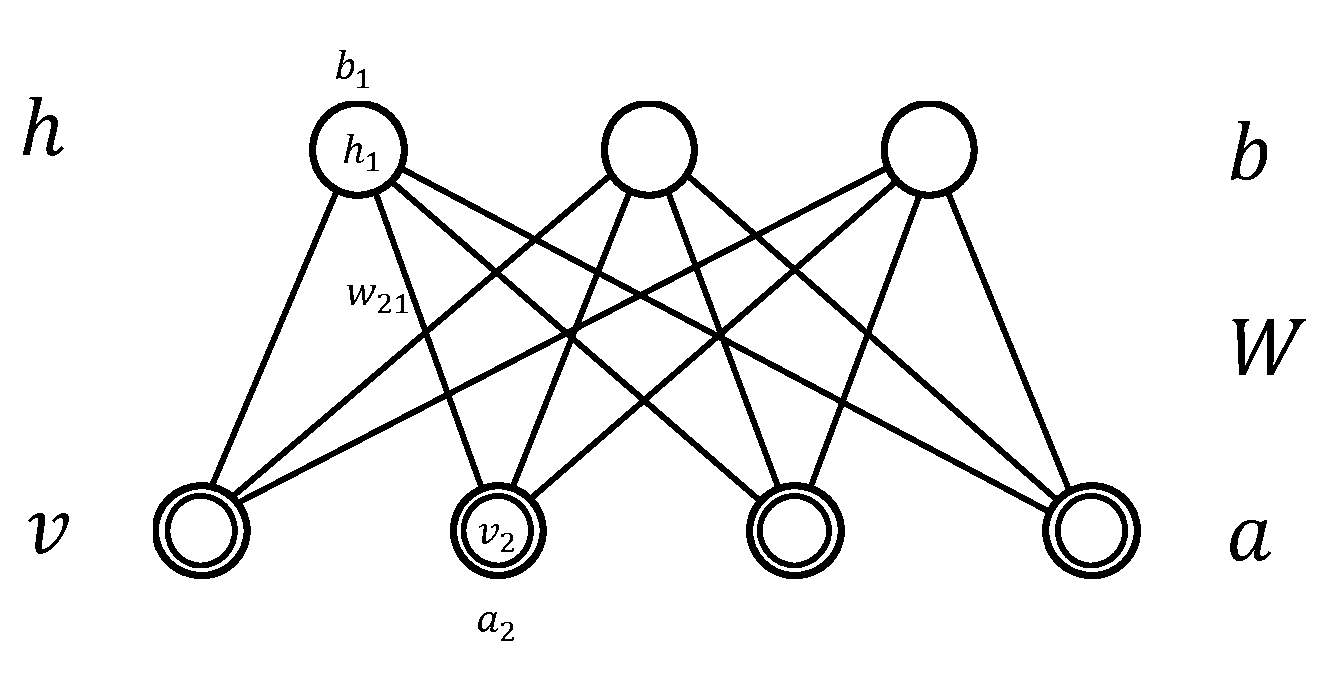
\includegraphics[scale=0.5]{images/rbmweights.pdf}
   \caption{The nodes and parameters of a restricted Boltzmann machine in the graph view. The second visible node and the first node in the hidden layer are connected with weight $w_{21}$ from the weight matrix $W$. The base-level activity of the nodes $v_2$ and $h_1$ is determined by the biases $a_2$ and $b_1$, respectively.}
   \label{fig:rbmweights}
 \end{figure}


Employing the sigmoid function $\sigm(x) = \frac{1}{1+ e^{-x}}$, the resulting conditional distributions can be written as 
\begin{equation}
p(v_i | h) = \sigm ((a + W h)_i)
 \quad \text{and}\quad 
p(h_i | v) = \sigm ((b + W^T v)_i).
\label{eqn:condprobrbm}
\end{equation}

The free energy is
\begin{equation}
F(v) = - a^T v - \sum_{j=1}^{n_H} \log \left (1 + e^{(W^T v + b)_j}\right).
\label{eqn:freenergy_rbm}
\end{equation}

The trick for deriving the formula of the free energy is to ``analytically sum out" the hidden units \citep{sala2012anefficient}.
The master thesis of \cite{krizhevsky2009tinyimagesthesis} is a very good resource for looking up the complete derivations of these formulas. This holds not only for the theory of RBMs with Bernoulli distributed nodes but also in particular for RBMs with Gaussian distributed visible nodes, which are presented next.

\paragraph{Gaussian distributed visible nodes for continuous data}
One way of modeling continuous values for $v$ are restricted Boltzmann machines with Gaussian distribution of the visible variables and Bernoulli distributed hidden variables. The energy of the model is defined as
\begin{equation}
   E(v,h) = \sum_{i=1}^{n_V}\frac{(v_i - a_i)^2}{2\sigma_i^2} - b^T h - \sum_{i=1}^{n_V} \frac{(Wh)_i}{\sigma_i}
   \label{eqn:energyformulagbrbm}
\end{equation}

The number of visible and hidden nodes is denoted as $n_V$ and $n_H$, respectively. The parameters of this model are $\Theta = (W, a, b, \sigma)$ with weight matrix $W$, visible bias $a$ hidden bias $b$ and standard deviation $\sigma$. The role of $\sigma$ as standard deviation becomes clearer by looking at the conditional distributions of the $v_i$ given $h$, which are distributed according to the normal distribution $\mathcal{N}(a_i + \sigma_i(Wh)_i, \sigma_i^2)$. For the hidden nodes, $p(h_j | v) = \sigm \left (b_j + \sum_{i=1}^{n_V} w_{ij} \frac{v_i}{\sigma_i} \right )$.
The free energy is
\begin{equation}
   F(v) = \sum_{i=1}^{n_V}\frac{(v_i - a_i)^2}{2\sigma_i^2} + \sum_{j=1}^{n_H} \log \left (1 + e^{b_j + \sum_{i=1}^{n_V} \frac{v_i}{\sigma_i} w_{ij}} \right).
\label{eqn:freenergy_gbrbm}
\end{equation}
\citep{krizhevsky2009tinyimages}.

Cho et al. \citep{cho2011improved} proposed a different parameterization for the energy function:
\begin{equation}
   E(v,h) = \sum_{i=1}^{n_V}\frac{(v_i - a_i)^2}{2\sigma_i^2} - b^T h - \sum_{i=1}^{n_V} \frac{(Wh)_i}{\sigma_i^2}
   \label{eqn:energyformulagbrbm2}
\end{equation}
In this model the distribution of the visible nodes is the multimodal normal distribution $\mathcal{N}(a + Wh, \sigma^2)$.
The conditional distribution of the hidden nodes is $p(h_j | v) = \sigm \left (b_j + \sum_{i=1}^{n_V} w_{ij} \frac{v_i}{\sigma_i^2} \right )$, and the free energy is
\begin{equation*}
   F(v) = \sum_{i=1}^{n_V}\frac{(v_i - a_i)^2}{2\sigma_i^2} + \sum_{j=1}^{n_H} \log \left (1 + e^{b_j + \sum_{i=1}^{n_V} \frac{v_i}{\sigma_i^2} w_{ij}} \right).
\end{equation*}

%TODO cite: 
%\citep{melchior_gbrbm}, \citep{cho_gaussiandbm}
% TODO mention alternative: use continuous as Gaussian hard., verweis auf entsprechenden results teil

\paragraph{Categorical data}\label{methodsoftmax0}
Another important statistical data type that needs to be handled when dealing with biomedical data is data with categorical values.
For most applications in machine learning, categorical data is usually encoded in dummy variables \citep{hastie_elements}.
It would be possible to use the binary dummy variables as input to a restricted or deep Boltzmann machine with Bernoulli distributed visible units as well.
But when sampling from such a Boltzmann machine model all combinations of visible nodes have a positive probability. This can be seen from the formula of the conditional probability (\ref{eqn:condprobrbm}) and the fact that the values of the sigmoid function are strictly positive.
Therefore, the resulting data is not properly encoded in general  because illegal combinations of dummy variables can occur. With that, sampled values cannot be mapped to the original categories any more.
Using dummy variables as input to Boltzmann machines with Bernoulli distributed variables makes it also more difficult to learn higher level patterns, as the Boltzmann machine has at first to learn the pattern that results from the dummy encoding  by itself. Hence it is advised to use a Boltzmann machine that has the knowledge about the encoding built into its energy function and probability distribution.


For encoding categorical variables, the most popular encoding used by the deep/machine learning frameworks \apkg{TensorFlow} \citep{tensorflow}, \apkg{scikit-learn} \citep{scikit-learn} or \apkg{Flux} \citep{flux} is the so-called ``one-hot encoding", which encodes a variable with $k$ categories in a binary vector of $k$ components, where exactly one component is one and all others are zero.
An advantage of this is that all categories are treated equally. 
Here, I tried a slightly different variant.
A categorical variables with $k$ categories is encoded in $k-1$ binary dummy variables.
This is the encoding of for values of a variable with four categories:

\begin{table}[h!]
\centering
\begin{tabular}{cc}
Categorical value & Dummy encoding \\
\hline
1 & 0 0 0 \\
2 & 1 0 0 \\
3 & 0 1 0 \\
4 & 0 0 1 \\
\end{tabular}
\caption{Dummy encoding with reference category for a categorical variable with four categories}\label{dummenc}
\end{table}

This variant is the same the technique for creating dummy variables for categorical variables in regression models \citep{faraway_regression}.
One category is used as reference category for the interpretation of the regression coefficients.
This allows to be parsimonious with parameters. Saving parameters can aid in training models also with fewer data points, as was shown with partitioning layers in DBMs \citep{hess2017partitioned}.
So there is the potential with this encoding to help also with learning on genetic data.
Consider genetic variant data that contains values 0/1/2 for each of defined location on the human genome to encode that there is no deviation from the reference genome (0), a deviation on one chromosome (1) or a deviation on both chromosomes (2).
An RBM receiving input with dummy encoding using the natural reference category 0 needs only two thirds of the parameters that an RBM needs which receives the same data in one-hot encoding.

The energy function $E$ for RBMs with categorical data is the same as for Bernoulli distributed visible nodes (see formula \ref{eqn:energyformularbm}).
The difference is that not all combinations of visible nodes are allowed. Thus the partition function $Z = \sum_{v} \sum_{h} e^{-E(v,h)}$ and the probability
$p(v) = \frac{\sum_h e^{-E(v,h)}}{Z}$ change because the sum over all possible states of $v$ in the formula for $Z$ contains less summands than in the case with a Bernoulli distribution, where all combinations of activations are possible.

For deriving the formulas for an RBM that handles the dummy encoding like exemplified in table \ref{dummenc}, let us denote with $C_k$ the set of dummy variables that the dummy variable $k$ belongs to.
The visible nodes of the RBM can cover multiple categorical variables and multiple sets of dummy variables, which may differ in the number of categories.
If the number of categories equals two for all categorical variables, this model is the same as an RBM with Bernoulli distributed nodes.

Like \cite{krizhevsky2009tinyimagesthesis} let us write $E(v_k = 1, v_{i \neq k}, h)$ for the energy of the combination of a visible vector $v$ with $v_k = 1$ and a hidden vector $h$. Similarly, let us define $E(v_{i \in C_k} = 0, v_{i \notin C_k}, h)$ for the energy of the combination of a visible vector $v$ that is zero in all dummy variables that belong to $C_k$ and a hidden vector $h$.

From the previously defined dummy encoding results that if one dummy variable in the set is one, all others in the set are zero. 
The sum over all possible combinations of $v$ can therefore be split into those parts where a dummy variable $k$ is zero and one part where all others in the corresponding set of dummy variables are one, because these covers all allowed combinations.
This allows to split the formula for the unnormalized probability of the hidden nodes into the following sum:
\begin{align}
p^*(h) &= \sum_v  \exp (-E(v,h)) \nonumber \\
&= \sum_{v_{i \notin C_k}} \exp (-E(v_{i \in C_k} = 0, v_{i \notin C_k}, h)) + \sum_{c \in C_k} \sum_{v_{i \notin C_k}} \exp ( - E(v_c = 1, v_{i \notin C_k},  h))
%E(v_k=1, v_{i\neq k}, h) = E(v_k = 1, v_{i \notin C_k}, h).
\end{align}

The input from the hidden nodes can further be extracted from $ \sum_{v_{i \notin C_k}} e^{-E(v_{k=1}, v_{i \neq k}, h)}$ by regrouping the summands:
\begin{align}
&\sum_{v_{i \notin C_k}} \exp ( - E(v_c = 1, v_{i \notin C_k},  h)) = \nonumber \\
&\quad = \sum_{v_{i \notin C_k}} \exp \left( \sum_{i \notin C_k} v_i h_j w_{ij} + \sum_{i \notin C_k} a_i v_i + a_k  + \sum_j h_j w_{kj} +\sum_j h_j b_j \right) \nonumber \\
&\quad = \exp \left( (Wh)_k + a_k \right) \sum_{v_{i \notin C_k}} \exp \left(-E(v_{i \in C_k} = 0, v_{i \notin C_k}, h) \right)
\label{eqn:sumvksoftmax}
\end{align}

The unnormalized probability $p^*(h)$ of the hidden nodes can now be rewritten as:

\begin{align}
p^*(h) =& \sum_{v_{i \notin C_k}} \exp (-E(v_{i \in C_k} = 0, v_{i \notin C_k}, h)) \; + \nonumber \\ 
&\quad  \sum_{c \in C_k} \left( (Wh)_c + a_c \right) \sum_{v_{i \notin C_k}} \exp \left(-E(v_{i \in C_k} = 0, v_{i \notin C_k}, h) \right)
\label{eqn:unnormalizedhiddensplit}
\end{align}

With this, the conditional probability of a dummy variable being one can finally be derived as follows:
\begin{align*}
p(v_k = 1 \mid h) &= \frac{p(v_k = 1, h)}{p(h)} \\
  &= \frac{p^*(v_k = 1, h)}{p^*(h)}\\
  &= \frac{\sum_{v_{i \notin C_k}} e^{-E(v_{k=1}, v_{i \neq k}, h)}}{p^*(h)} \\
 %&=  \frac{\sum_{v_{i \notin C_k}} \exp \left( \sum_{i \notin C_k} v_i h_j w_{ij} + \sum_{i \notin C_k} a_i v_i + a_k  + \sum h_j w_{kj} +\sum_j h_j b_j \right)}{p^*(h)} \\
 &\stackrel{(\ref{eqn:sumvksoftmax})}{=} \frac{\exp \left( (Wh)_k + a_k \right) \sum_{v_{i \notin C_k}} \exp \left(-E(v_{i \in C_k} = 0, v_{i \notin C_k}, h) \right)}{p^*(h)}\\
&\stackrel{(\ref{eqn:unnormalizedhiddensplit})}{=} \frac{\exp((Wh)_k + a_k)}{1 + \sum_{c \in C_k} \exp ((Wh)_c + a_c)}
  %&= \frac{\exp \left( (Wh)_k + a_k \right) \sum_{v_{i \notin C_k}} \exp \left(-E(v_{i \in C_k} = 0, v_{i \notin C_k}, h) \right)}{\sum_{u_{i\notin C_k)}
\end{align*}

\subsubsection{Gibbs sampling in restricted Boltzmann machines}\label{gibbssamplingrbm}
To use RBMs as generative models, one must be able to draw samples from the distribution captured in the parameters of the model.
The straightforward way would be to calculate $p(v)$ and sample according to this distribution.
But $p(v)$ depends on the partition function $Z$ and calculating $Z$ is not feasible for most practical scenarios, as the number of summands in $Z$ grows exponentially with the number of nodes in the model (see also later in \ref{methodExactloglik}).
Because of the layered structure of RBMs and the closed form of the conditional distributions $p(v \mid h)$ and $p(h \mid v)$, which is fast to evaluate, it becomes possible to apply a Markov chain Monte Carlo technique called \emph{Gibbs sampling} \citep{gibbssamplingorig}.

The Gibbs sampling  algorithm for RBMs can be formulated as follows:

\begin{enumerate}
\item Start with an arbitrary $v_1$.
\item Draw $h_1$ according to $p(h \mid v_1)$.
\item Draw $v_2$ according to $p(v \mid h_1)$.
\item Repeat steps 2 and 3 until convergence.
\item Result: After $n$ steps, $v_n$ and $h_n$ have been drawn according to the joint distribution $p(v,h)$ of the model.
\end{enumerate}

This works because the iteration forms a Markov chain, which has the distribution $p(v,h)$ of the model as its equilibrium distribution.

\paragraph{Conditional sampling}
The Gibbs sampling algorithm can also be easily modified for \emph{conditional sampling} by clamping the activations of the nodes that are to be conditioned on.
Put more formally, to draw from the probability $p(v, h \mid \tilde{v}_C)$ that is conditioned on the activations $\tilde{v}_C$ of a set $C$ of visible nodes, the Gibbs sampling algorithm above can be run with $v_C$ set to $\tilde{v}_C$ in step 1 and after each sampling step 3.
This, of course, works analogously for hidden nodes as conditions.

An example for using conditional sampling in a setting with biomedical data could be the simulation of a patient cohort with a specific rare disease pattern using a Boltzmann machine that has been trained with a data set of diagnoses from a more general population cohort.
A result from such a simulation could be used for a case number calculation when planning a study involving the specific disease pattern and other combinations of characteristics.
As the combinations might be quite rare, the learned correlations between all the variables can help in estimating the frequencies of the combinations of specific characteristics.

\subsubsection{Training of restricted Boltzmann machines}\label{rbmtraining}
Goal of the training procedure of restricted Boltmann machines is to maximize the likelihood $\prod_{k=1}^n p(\widetilde{v}_k)$ for a given data set $(\widetilde{v}_1, \dots, \widetilde{v}_n)$.
As mentioned in section \ref{basicbmproperties}, calculating $p(v) = \frac{\sum_{h} p(v,h)}{Z}$ needs the partition function $Z$.
Maximizing the likelihood is equal to maximizing the log-likelihood
\[
\sum_{k=1}^{n}  \log p(\widetilde{v}_i) = \sum_{k=1}^{n} \left( \log \sum_h e^{-E(\widetilde{v}_k, h)} - \log \sum_v \sum_h e^{-E(v, h)} \right)
\]

\paragraph{Deriving the gradient of the log-likelihood}


For finding an optimum, the gradient $\nabla_\Theta \sum_{k=1}^{n}  \log p_\Theta(\widetilde{v}_k)$ needs to be determined.
The negative of gradient of the log-likelihood for a single observation
$\widetilde{v} $ with respect to the parameters $\Theta$ is
\begin{align}
- \nabla_{\!\Theta}  \log p(\widetilde{v}) &= - \nabla_{\!\Theta}   \log \sum_h e^{-E(\widetilde{v}, h)} + \log \sum_v \sum_h e^{-E(v, h)} \nonumber \\
 &= - \frac{\nabla_{\!\Theta} \sum_h e^{-E(\widetilde{v}, h)}}{\sum_h e ^{-E(\widetilde{v}, h)}}  + \frac{\nabla_{\!\Theta} \sum_v \sum_h e^{-E(v,h)}}{\sum_v \sum_h e^{-E(v,h)}} \label{eqn:derivedlog}\\
&=  \frac{\sum_h e^{-E(\widetilde{v}, h)} \nabla_{\!\Theta} E(\widetilde{v}, h)} {\sum_h e^{-E(\widetilde{v}, h)}} - \frac{\sum_v \sum_h e^{-E(v, h)} \nabla_{\!\Theta} E(v, h)}{\sum_v \sum_h e^{-E(v, h)}} \label{eqn:derivedexp}\\
&=  \EX_{P_\text{data}} \nabla_{\!\Theta} E(\widetilde{v},h) - \EX_{P_\text{model}} \nabla_{\!\Theta} E(v,h) \label{eqn:nablaresult}
\end{align}
In (\ref{eqn:derivedlog}) and (\ref{eqn:derivedexp}), the chain rule is used, together with the derivative of the logarithm and the exponential function, respectively. The resulting terms can be rewritten in equation (\ref{eqn:nablaresult}) as the expectation of the gradient given the distribution of the data and the expectation of the gradient given the distribution of the model.

As can be seen in equation (\ref{eqn:derivedexp}), the calculation of the gradient involves sums over lots of possible combinations of activations of nodes.
The first term can be calculated in the types of RBMs that have been introducted here.
For this, one can use the expected value of the conditional probability $p(h\mid\widetilde{v})$ and plug it in:
\[
\EX_{P_\text{data}} \nabla_{\!\Theta} E(\widetilde{v},h) =  \nabla_{\!\Theta} E(\widetilde{v}, \EX(p(h \mid \widetilde{v}))
\]
In the second term of equation (\ref{eqn:nablaresult}), the sum goes over all nodes in the network.
Calculating this term is technically not feasible in normal cases, as the number of summands grows exponentially with the number of nodes.
This means that it is not possible to simply equate the gradient of the log-likelihood with zero and solve the equation to get an optimum. Also finding an optimum with gradient descent, walking with small steps in the direction of the gradient to find an optimum, is not possible directly, because this would as well require the calculation of the whole gradient in each iteration step.
Via Gibbs sampling (see section \ref{gibbssamplingrbm}), however, the term can be estimated. 
With this, it becomes possible to use the estimated gradients in gradient descent, or here rather ``gradient ascent" as we would like to find a (local) maximum.

\paragraph{Batch gradient optimization and the role of mini-batches}

For the practical implementation, another stochastic approximation of the gradient for the full data set $\sum_{k=1}^n \log p(\widetilde{v}_i)$ is used.
Usually a form of {\em batch gradient optimization} \citep{bottou_optimization_2018} is performed.
For this, the samples are split into batches $B_l$, usually of approximately equal sizes $b_l$.
In each optimization step $t$, the parameters are updated as follows:
\[
\Theta^{(t+1)} = \Theta^{(t)} + \frac{\epsilon}{b_l} \sum_{\widetilde{v} \in B_l} \nabla_{\!\Theta} \log p(\widetilde{v})
\]

The step size is determined by the {\em learning rate} $\epsilon$.
Each iteration $t$ calculates the gradient of a different batch $B_l$ until all samples have been used.
The mini-batches are usually reused multiple times for the learning.
The number of steps after all samples/mini-batches are used for updating the parameters, is called a {\em (training) epoch}.
(In the formula above one training epoch is over if $t = \sum_l b_l$.)
Training usually consists of many epochs and the step size is kept small, e.g. a hundred epochs and a learning rate of 0.001 could be a viable combination.
The number of epochs and the learning rate are the most important hyperparameters for the training.

%TODO optional: hier könnte man mehr schreiben über zusammenspiel von learning rate und epochs, außerdem steps auf oberfläche beschreiben und learning rate decay

Mini-batches are at first introduced for performance reasons.
It is not necessary to have the exact gradient for walking only small steps into the direction of it.
So it is sufficient to calculate the gradient for small subsets of the data, which is noisy, but will be correct on average.
Using mini-batches can also be advantageous because of another reason: The variance of the steps becomes higher with a with a smaller batch size. This leads to exploring more of the surface of the likelihood function in the high-dimensional space and therefore can lead to finding better local optima in some scenarios \citep{bengio2012practical}.

\paragraph{Contrastive divergence}

For performing batch gradient optimization, the Gibbs sampling procedure is also modified for RBM training to speed up the learning process.
In other applications, thousands of iterations are used for Gibbs sampling  \citep{gibbssamplingorig}. For training RBMs, a shortcut is used, which is called {\em contrastive divergence} (CD) \citep{cdorig, perpinan_contrastive_2005}.
In CD, the number of Gibbs sampling steps is reduced drastically. In most cases, even only one step is used, which is denoted with $\text{CD}_1$ \citep{hinton_practical_2012}.
Instead of using a random starting point, CD uses the original sample $\widetilde{v}$, for which the gradient shall be computed, as starting point $v_1$ of the sampling procedure. This should ensure that the starting point is already close to the desired distribution.

Another modification of the Gibbs sampling procedure used for training of RBMs is {\em persistent contrastive divergence} (PCD).
Similar to CD, this procedure also uses only very few steps. Here, the state of the Gibbs sampling chain for calculating the last update is reused and used as starting point. \cite{hinton_practical_2012} recommends PCD over $\text{CD}_1$ or even $\text{CD}_{10}$.

\paragraph{Gradients for different types of restricted Boltzmann machines}

In an RBM with Bernoulli distributed nodes, equation (\ref{eqn:nablaresult}) leads to the following formulas for the negative gradients for the weights and biases:
\begin{align*}
- \frac{\partial}{\partial W}  \log p(\widetilde{v}) &= \EX_{P_\text{data}}  \widetilde{v}^T h - \EX_{P_\text{model}} v^T h \\
- \frac{\partial}{\partial a}  \log p(\widetilde{v}) &=  \EX_{P_\text{data}} 
\widetilde{v} - \EX_{P_\text{model}}  v = \widetilde{v} - \EX_{P_\text{model}} v\\
- \frac{\partial}{\partial b}  \log p(\widetilde{v}) &=  \EX_{P_\text{data}} h - \EX_{P_\text{model}} h 
\end{align*}

In an RBM with Gaussian visible nodes \citep{krizhevsky2009tinyimagesthesis}, the negative gradients are:
\begin{align*}
- \frac{\partial}{\partial W} \log p(\widetilde{v}) &= \frac{1}{\sigma_i} \left ( \EX_{P_\text{data}} \widetilde{v}^T h - \EX_{P_\text{model}} v^T h \right) \\
- \frac{\partial}{\partial a} \log p(\widetilde{v}) &= \frac{1}{\sigma_i^2} \left(\widetilde{v} - \EX_{P_\text{model}} v \right)\\
- \frac{\partial}{\partial b} \log p(\widetilde{v}) &= \EX_{P_\text{data}} h - \EX_{P_\text{model}} h \\
- \frac{\partial}{\partial \sigma_{i}} \log p(\widetilde{v}) &= \EX_{P_\text{data}} \left( \frac{(\widetilde{v}_i - a_i)^2}{\sigma_i^3} - \sum_{j=1}^{n_H} h_j \frac{w_{ij} \widetilde{v}_i}{\sigma_i^2}\right) \\ & \quad \quad - \EX_{P_\text{model}} \left(\frac{(v_i - a_i)^2}{\sigma_i^3} -\sum_{j=1}^{n_H} h_j \frac{w_{ij} v_i}{\sigma_i^2} \right)
\end{align*}

In the alternative formulation of \cite{cho2011improved}, the negative gradients are:
\begin{align*}
- \frac{\partial}{\partial W} \log p(\widetilde{v}) &= \frac{1}{\sigma_i^2} \left ( \EX_{P_\text{data}} \widetilde{v}^T h - \EX_{P_\text{model}} v^T h \right) \\
- \frac{\partial}{\partial a} \log p(\widetilde{v}) &= \frac{1}{\sigma_i^2} \left(\widetilde{v} - \EX_{P_\text{model}} v \right)\\
- \frac{\partial}{\partial b} \log p(\widetilde{v}) &= \EX_{P_\text{data}} h - \EX_{P_\text{model}} h \\
- \frac{\partial}{\partial \sigma_{i}} \log p(\widetilde{v}) &=  \frac{1}{\sigma_i^3} \Bigg( \EX_{P_\text{data}} \left( (\widetilde{v}_i - a_i)^2 - 2\sum_{j=1}^{n_H} h_j w_{ij} \widetilde{v}_i  \right) \\ & \quad \quad - \EX_{P_\text{model}} \left((v_i - a_i)^2 -2\sum_{j=1}^{n_H} h_j w_{ij} v_i \right) \Bigg)
\end{align*}

In the RBM with the dummy variables for encoding categorical variables, the gradients are the same as in the one with Bernoulli distributed variables.

\subsubsection{Deep belief networks}

The next step in the evolution of Deep belief networks (DBNs) \citep{hinton_reducing_2006}.

\subsubsection{Deep Boltzmann machines}

A deep Boltzmann machine, as defined by \cite{salakhutdinov2009DBMs}, with $n_L$ number of hidden layers has parameters 
\[
\Theta = \left (W^{(1)}, \dots, W^{(n_L)}, a, b^{(1)}, \dots, b^{(n_L)} \right).
\]
The energy is defined as 
\[
E(v, h^{(1)}, \dots, h^{(n_L)}) = - a^T v - v^T W^{(1)} h^{(1)} - \sum_{k=1}^{n_L} b^{(k)} h^{(k)} -  \sum_{k=2}^{n_L} h^{(k-1)}W^{(k)}h^{(k)}.
\]
For the connection between the formula and the resulting network architecture see figure  \ref{fig:dbmweights}.
\begin{figure}[h]
   \centering
   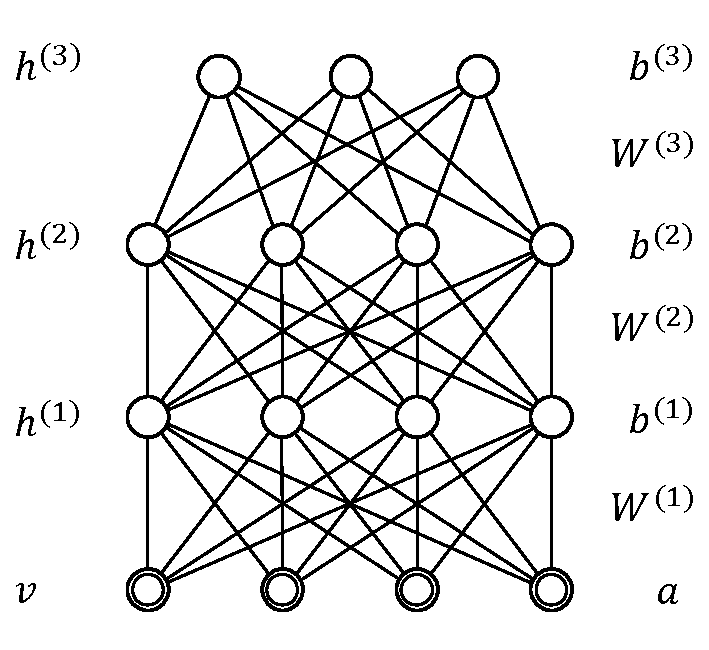
\includegraphics[scale=0.6]{images/dbmweights.pdf}
   \caption{The nodes and parameters of a deep Boltzmann machine in the graph view}
   \label{fig:dbmweights}
 \end{figure}
 
A deep Boltzmann machine has Bernoulli distributed nodes.
Due to the layer-wise structure, the conditional probability of the visible nodes $p(v \mid h) = p(v \mid h^{(1)})$ depends only on the first hidden layer and can be calculated like in an RBM with Bernoulli distributed nodes.
The conditional probability of the final hidden layer $p \left( h^{n_L} \mid v, h^{(1)}, \dots, h^{(n_L -1)} \right) = p \left( h^{n_L} \mid h^{(n_L -1)} \right)$ can similarly be calculated by knowing only on $h^{(n_L-1)}$.
For the intermediate layers, the conditional probability can be calculated if the neighboring layers are given as
\[
p\left(h^{(1)} \mid v, h^{(3)}\right) = \sigm \bigg( b^{(1)} + (W^{(1)})^T v + W^{(3)} h^{(3)} \bigg)
\]
for the first hidden layer and 
\[
p\left(h^{(k)} \mid h^{(k-1)}, h^{(k+1)} \right) = \sigm \bigg( b^{(k)} + (W^{(k-1)})^T h^{(k-1)} + W^{(k+1)} h^{(k+1)} \bigg)
\]
for all other intermediate hidden layers.


\subsubsection{Multimodal deep Boltzmann machines}

The energy function of a multimodal deep Boltzmann machine (MDBM) is TODO


\subsubsection{Training of deep Boltzmann machines}

For pre-training the multimodal deep Boltzmann machines, we use greedy layerwise pre-training  of layers of restricted Boltzmann machines.
DBN \citep{hinton_reducing_2006}
Fine-tuning of weights can then be performed by the algorithm for training a general Boltzmann machine.
\citep{salakhutdinov2009DBMs, salakhutdinov2015generativemodels}
This algorithm is also based on stochastic gradient descent.
Calculating the derivative in deep Boltzmann machines needs an additional technique.

When training with the mean-field approximation $\mu$ used as activation of the hidden nodes in the positive phase,
the likelihood is not optimized directly but a lower bound
\[
   \log p(v) \geq - E(v, \mu) - \log Z + \mathcal{H}(\mu)
\]
is optimized. $\mathcal{H}$ denotes the entropy of the hidden nodes. \citep{sala2012anefficient}

TODO parameter updates
TODO stacking
TODO Referenz zu Srivastava
Since the training procedure is very complex and depends on many hyperparameters, it is necessary to test whether the training works well by examining the training objective.
Although the likelihood is not the best criterion for all kinds of applications \citep{theis_note_2015}, it is essential to have a way to get a value for the likelihood as primary optimization criterion.
Being able to inspect the learning process is important for finding the best choice of hyperparameters and also for ensuring the quality of the software implementation of the learning algorithm.
This leads us to the next section, where we want to take a closer look at methods for calculating and estimating the likelihood, and lower bound of the likelihood, in case DBMs.


\subsubsection{Evaluating restricted and deep Boltzmann machines}
A special challenge for unsupervised learning on non-image data in general is the lack of performance indicators.
In supervised training, the classification accuracy is the natural evaluation criterion, which is also easy to implement.
In unsupervised training with a well investigated class of data such as images, there is already much experience available for choosing the model architecture and the hyperparameters. If models are to be trained on very diverse data, the problem of finding good hyperparameters is exacerbated as parameter tuning can pose a different challenge for each data set.

Thus the need for having an objective evaluation criterion as a basis for choosing the hyperparameters and monitoring the training becomes very important.
In case of images or natural language, the generative abilities of a model can be tested by simply looking at the generated images or sentences to see whether these are proper samples. In the case of data from a patient record or genetic data, this approach is not feasible.

If there are no other evaluation criteria, one indicator for successful learning in Boltzmann machines remains the model likelihood, which is an inherent property of the model and is therefore applicable in all cases of data. The difficulty for calculating the likelihood is its dependency on the partition function (see formula (\ref{eqn:probbm})).
In most cases, the likelihood cannot be calculated exactly but it can only be estimated by stochastic algorithms like annealed importance sampling (AIS). 
% So we also want to detail the extension of AIS on multimodal deep Boltzmann machines in this article.

\paragraph{Exact calculation of the partition function}
\label{methodExactloglik}
As mentioned in section \ref{rbmtraining}, the exact calculation of partition functions is only computationally feasible for very small models as its complexity grows exponentially. Exploiting the layerwise structure allows a faster exact calculation of $Z$ such that the computation time does not grow exponentially with the number of all nodes but only grows exponentially with the number of elements in a subset of the nodes. It is possible to utilize the formula for the free energy in restricted Boltzmann machines (see formulas (\ref{eqn:freenergy_rbm}) and (\ref{eqn:freenergy_gbrbm})), where the hidden layer is summed out analytically.
With this it is possible to reduce the number of summands. 
The complexity for calculating the partition function for all the different types of  models described here is then still $\mathcal{O}(2^n)$, but with an $n$ smaller than the number of nodes:

By using the formulas for the free energy and the symmetry of restricted Boltzmann with binary nodes, $n = \min(n_V, n_H)$ with $n_V$.
In RBMs with one of layer Gaussian nodes and one layer of binary nodes, $n$ is the number of binary nodes, since the contribution of the Gaussian nodes can be integrated analytically.
In case of a deep Boltzmann machine, it is possible to sum out each second layer, similar to the calculation of the free energy in restricted Boltzmann machines. So for DBMs, $n$ can be reduced to the number of nodes in each second layer, see figure \ref{aissummingout}.

\begin{figure}[h!]
\centering
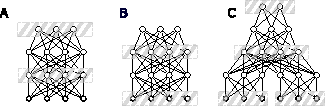
\includegraphics[scale=2.5]{images/AISsummingout.pdf}
\caption{Possibilities for summing out layers for calculating the likelihood. For calculating the likelihood in a more efficient way, the layers in the gray boxes can be summed out analytically. {\bf A:} Summing out the odd layers in this DBM leaves $2^{(4 + 4)} = 256$ summands that still have to be summed in order to calculate the likelihood. {\bf B:} Summing out the even layers in this DBM leaves in $2^{(4 + 3)} = 128$ summands. {\bf C:} Summing out the even layers in  this multimodal DBM leaves $2^{(6 + 3)} = 512$ summands.}
\label{aissummingout}
\end{figure}

\paragraph{Estimating partition functions with annealed importance sampling (AIS)}\label{methodAIS}

For annealed importance sampling we need a sequence of intermediate distributions
$p_0, \dots p_K$ with
$p_0 = p_A$ and $p_K = p_B$. The ratio $\frac{Z_B}{Z_A}$ is then estimated by the mean of a number of so called importance weights that are determined as
\[
   \prod_{k=1}^K \frac{p^*_k(x_k)}{p^*_{k-1}(x_{k})}.
\]
The $x_k$ are produced by iteratively performing Gibbs sampling. Starting with $x_0$ sampled from $p_0$, one obtains $x_k$ by sampling a Gibbs chain that is initialized with $x_{k-1}$ in an intermediate model with distribution $p_k$. An appropriate choice for the intermediate models are Boltzmann machines with the energy functions $E_k$ chosen such that
\[
   E_k(x) = (1 - \beta_k) E_A(x) + \beta_k E_B(x)
\]
and therefore
\[
   p_k^*(x) = p_A^*(x)^{1-\beta_k} p_B^*(x)^{\beta_k}.
\]
The factors $\beta_k$ with $0 = \beta_0 < \beta_1 < ... < \beta_K = 1$ are called temperatures \citep{salakhutdinov2008learning}.
The choice of the temperatures, the number of importance weights and also the number of Gibbs sampling steps for the transition are hyperparameters for the AIS algorithm.

With AIS, it is possible to get a direct estimate of $Z$ by annealing from the full model with distribution $p_A$ to a null model with all weights being zero, for $p_B$.
The partition function $Z_B$ of the null model can be calculated directly, and therefore $Z_A$ can be computed from the AIS estimator of $\frac{Z_B}{Z_A}$. This approach is shown in figure \ref{figTwotypesais}A.

It is also possible to compare the likelihood of two models instead of calculating it directly.
For this, only the ratio $\frac{Z_B}{Z_A}$ between two full models needs to be estimated.
There are two practical approaches for constructing intermediate models  for directly annealing from one full model to another full model (see also figure \ref{figTwotypesais}, B and C):
\begin{enumerate}
\item Combining (adding) corresponding weights of two models of the same size to get an intermediate model of the same size.
\item Constructing a larger model by putting the two models next to each other and connecting their nodes, increasing the energy in one part of the combined model while reducing it in the other part \citep{theis2011deepbelief}:
\end{enumerate}
\begin{figure}[h!]
\centering
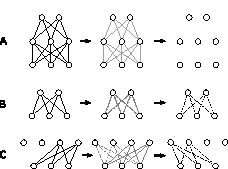
\includegraphics[scale=3.5]{images/twotypesais.pdf}
\caption{Different approaches for performing AIS. 
The tempered weights of the intermediate distributions are shown in grey. Black lines correspond to the original weights of a model. No lines between nodes are equal to the weights being zero.
{\bf A:} Annealing from a null model, where all weights are zero, to the full model.
{\bf B:} Annealing from one RBM model with three visible nodes and two hidden nodes to another model of the same size.
The weights of the first model are depicted as continuous lines, the weights of the second as dashed lines. Here, model one is gradually morphed into model two. {\bf C:} 
The same two RBMs are compared again by annealing from a model that is equivalent to the first model to a model that is equivalent to a second model via a combined, bigger model. For this approach, both models do not necessarily have to be of the same size.}
\label{figTwotypesais}
\end{figure}
The approach with a combined model (see figure \ref{figTwotypesais}C) is more flexible and allows to estimate the ratios of two arbitrary Boltzmann machines of the same type and with the same number of hidden nodes.
But it requires sampling in a Boltzmann machine that has as many hidden nodes as the two models together.

% TODO verweis, was im package benutzt wird.


In a DBM, it is possible to use only the states of each second layer from samples generated by running a Gibbs chain \citep{salakhutdinov2008learning}. The unnormalized probabilities of these states can be calculated by analytically summing out the other layers.
For this, we can use the fact that the states in one layer are independent from the states of each non-adjacent layer to get the unnormalized probability $p_k^*(\tilde{h})$ for the subset $\tilde{h} = \left(h^{(1)}, h^{(3)}, \dots\right)$ of a generated sample $x = \left( v, h^{(1)}, h^{(2)}, \dots \right)$ in an intermediate model. 
The layers that can be analytically summed out are the same as the ones shown in figure \ref{aissummingout}.
To calculate the ratio $\frac{p_k^*(x_k)}{p_{k-1}^*(x_{k})}$, one can derive the formula for $p^*(\tilde{h})$ in a DBM similarly to the free energy $F(v) = - \log p^*(v)$ in RBMs \citep{sala2012anefficient}. For a DBM with three hidden layers, the formula is
\begin{align}
p^*( \tilde{h} ) =&  e^{(b^{(1)})^T h^{(1)}} \prod_j (1+ \exp((a + W^{(1)} h^{(1)})_j)) \; \cdot \nonumber \\ 
&e^{(b^{(3)})^T h^{(3)}} \prod_{j}  \left( 1 + \exp \left( (b^{(2)} + (W^{(2)})^T h^{(1)} + W^{(3)} h^{(3)})_j \right) \right).
\label{eqn:aisunnormalizedprob}
\end{align}

Here the visible layer $v$ and the second hidden layer $h^{(2)}$ have been summed out analytically, like shown in figure \ref{aissummingout}B.

%Note that the model for Gibbs sampling, used as the Markov transition operator, can differ from the model that is used to evaluate the unnormalized probability $p_k^*(h)$ as long as the probability distribution $p_k(h)$ of the hidden nodes is the same.
%This trick can be used to fit AIS for GBRBMs in the same schema as RBMs with Bernoulli distributed nodes.
It can be noted that the term in the first line of formula \ref{eqn:aisunnormalizedprob} is equal to the unnormalized probability of the hidden nodes in a RBM with Bernoulli distributed nodes.
This procedure can be generalized for AIS on multimodal DBMs. 
If we have the unnormalized probability $p^*(h)$ for each type of RBM that receives the data input, it becomes possible to calculate the unnormalized probability of sampled hidden values in a multimodal DBM in the same way as for a standard DBM with only Bernoulli distributed nodes.
The formula for the unnormalized probability for the respective RBM type (see section \ref{unnormalizedprobsrbm}) can then be used for summing out the visible units in formula \ref{eqn:aisunnormalizedprob} by substituting the term in the first line with the product of the unnormalized probabilities for all RBMs in the visible layer.

The formulas for $p^*(h)$ for each different type of RBM are derived next, also by analytically ``summing out", or in case of Gaussian RBMs, ``integrating out" the visible layer.

\paragraph{Derivation of unnormalized probability for different types of restricted Boltzmann machines}\label{unnormalizedprobsrbm}

Due to the symmetry of hidden and visible nodes in a RBM with only {\bf Bernoulli distributed nodes}, $p^*(h)$ can be derived analogously to the free energy $F(v) = - \log p^*(v)$ in this case.

Since I have not found formulas for the unnormalized probability of the hidden nodes in RBMs with Gaussian visible nodes in the literature, I derive it here in detail.
The derivations for $p^*(h)$ for RBMs with Gaussian visible nodes use the fact that the integral over the density function of a normal distribution $\mathcal{N}(\mu, \sigma^2)$ is equal to one:
\begin{equation} \int \frac{1}{\sqrt{2 \pi \sigma^2}} e^{ -\frac{(x - \mu)^2}{2 \sigma^2}} = 1  
\label{eqn:densitynormal}
\end{equation}

With that, the unnormalized probability of the hidden nodes in a {\bf Gaussian RBM with original parameterization} (see formula (\ref{eqn:energyformulagbrbm})) can be calculated as

\begin{align*}
   p^*(h) &= \int e^{-E \left(v,h \right)} dv \\
   &= \int \exp \left( -\sum_{i=1}^{n_V}\frac{(v_i - a_i)^2}{2\sigma_i^2} + b^T h + \sum_{i=1}^{n_V} \sum_{j=1}^{n_H} \frac{v_i}{\sigma_i}h_j w_{ij} \right) dv\\
   &= e^{b^T h} \int \exp \left( \frac{v_i^2 -2 a_i v_i + a_i^2 - 2 v_i (Wh)_i \sigma_i}{2 \sigma_i^2} \right) dv \\
   &= e^{b^T h} \int \exp \left(
      - \sum_{i=1}^{n_V} \frac{{\left( v_i - \left( (Wh)_i \sigma_i + a_i \right) \right)}^2}{2\sigma_i^2} + \frac{1}{2}(Wh)_i^2 + (Wh)_i \frac{a_i}{\sigma_i} \right ) dv \\
   \begin{split}
      &= \exp \left(b^T h + \sum_{i=1}^{n_V} \frac{1}{2}(Wh)_i^2 + (Wh)_i \frac{a_i}{\sigma_i} \right ) \cdot \\
      & \quad \quad \int \exp \left ( - \sum_{i=1}^{n_V} \frac{{\left( v_i - ((Wh)_i \sigma_i + a_i) \right)}^2}{2\sigma_i^2} \right) dv
   \end{split} \\
   & \stackrel{(\ref{eqn:densitynormal})}{=} \exp \left( b^T h + \sum_{i=1}^{n_V} \frac{1}{2}(Wh)_i^2 + (Wh)_i \frac{a_i}{\sigma_i} \right ) \prod_{i=1}^{n_V}\left(\sqrt{2\pi} \sigma_i\right). \\
\end{align*}

For {\bf Cho's alternative parameterization} (see formula (\ref{eqn:energyformulagbrbm2})), the unnormalized probability calculates analogously as
\begin{align*}
   p^*(h) &= \int e^{-E \left(v,h \right)} dv \\
   &= \int \exp \left( - \sum_{i=1}^{n_V} \frac{(v_i - a_i)^2}{2\sigma_i^2} + \sum_{i=1}^{n_V} \sum_{j=1}^{n_H} h_j w_{ij} \frac{v_i}{\sigma_i^2} - \sum_{i=1}^{n_H} b_j h_j \right) dv \\
   &= e^{b^T h} \int \exp\left( - \sum_{i=1}^{n_V} \frac{(v_i - a_i)^2 - 2 v_i (Wh)_i}{2 \sigma_i^2} \right) dv \\
   &= e^{b^T h} \int \exp \left( - \sum_{i=1}^{n_V} \frac{\left((v_i - ((Wh)_i + a_i) \right)^2}{2 \sigma_i^2}  + \sum_{i=1}^{n_V} \frac{(Wh)_i^2 + 2 a_i (Wh)_i}{2\sigma_i^2} \right) dv\\
   &= \exp \left( b^T h + \sum_{i=1}^{n_V} \frac{(Wh)_i^2 + 2 a_i (Wh)_i}{2\sigma_i^2} \right) \cdot \\
   & \quad \quad \int \exp \left(- \sum_{i=1}^{n_V} \frac{\left((v_i - ((Wh)_i + a_i) \right)^2}{2 \sigma_i^2} \right) dv\\
   &\stackrel{(\ref{eqn:densitynormal})}{=} \exp \left( b^T h + \sum_{i=1}^{n_V} \frac{\frac{1}{2}(Wh)_i^2 + (Wh)_i a_i}{\sigma_i^2} \right ) \prod_{i=1}^{n_V}\left(\sqrt{2\pi} \sigma_i \right).
\end{align*}

For the RBM for {\bf categorical variables with the dummy encoding with reference level} from section \ref{methodsoftmax0}, the unnormalized probability can be derived similar to the RBM with Bernoulli distributed nodes. At first, the energy function can be rewritten in the same way as with the RBM with Bernoulli distributed nodes:
\begin{align}
e^{-E(v,h)} &= \exp \left(\sum_j b_j h_j + \sum_{i,j} w_{ij} v_i h_j + \sum_i a_i v_i \right) \nonumber \\
&= \exp \left( \sum_i b_j h_j + \sum_i v_i \left( a_i + \sum_j w_{ij} h_j \right) \right) \nonumber \\
&= e^{\sum b_h h_j} \prod_i \underbrace{e^{v_i (a_i + \sum_j w_{ij} h_j)}}_{(*)}
\label{eqn:freeenergytrick}
\end{align}
\begin{equation*}
(*) = \left\{
\begin{array}{l}
 =1 \text{ for } v_i = 0 \\
 = e^{a_i +\sum_j w_{ij} h_j} \text{ for } v_i = 1 
\end{array} \right.
\end{equation*}

When multiplying out the product below using equation (\ref{eqn:freeenergytrick}), it can be seen that $p^*(h)$ can be written as
\begin{align*}
p^*(h) &= \sum_v e^{-E(v,h)} \\
&= e^{\sum_j b_j h_j} \prod_{C} \left( 1 + \sum_{i \in C} e^{\sum_j w_{ij} h_j + a_i} \right).
\end{align*}
Here $C$ denotes the set of all index sets of the dummy variables, where each index set belongs to a categorical variable.


\paragraph{Calculating or estimating likelihoods in deep Boltzmann machines} %TODO verbessern
For a restricted Boltzmann machine, the likelihood can be calculated using formula (\ref{eqn:pRBMfreeenergy}) if the partition function is known. This is not so easily possible in a DBM, for which calculating the distribution of the hidden nodes is of exponential complexity.
Estimating the likelihood of DBMs is possible using AIS by constructing a smaller DBM for each sample and estimating its partition function.
The smaller DBM is constructed by removing the visible layer, and incorporating contribution of the sample to the energy of the first RBM - consisting only of visible and first hidden layer - into the bias of the new visible layer which was the first hidden layer of the original model.
The partition function of this smaller model is then the unnormalized probability of the sample in the original model.
In a setting with very large sample size, the cost of estimating the actual likelihood with this procedure is too expensive. But if the sample size is small enough, it is affordable to estimate the likelihood and not fall back on the lower bound.

\paragraph{Alternatives to the likelihood}
The AIS algorithm is very complex to implement.
It is also compute-intensive, depending on the required exactness of the estimation.
So often there are other statistics used for checking the training progress.

The free energy cannot be used for comparing different models because it does not include the normalization by $Z$.
It can, however, be used to compare how well the same model fits different data sets.
One application for this is monitoring the overfitting by comparing the training data set and a test data set \citep{hinton_practical_2012}.

Another popular statistics, which behaves similar to the likelihood in RBMs in most cases, is the {\em reconstruction error} \citep{hinton_practical_2012}.
For defining this, one needs at first to define the term {\em reconstruction} in an RBM.
The reconstruction \citep{hinton_practical_2012} for a sample $\widetilde{v}$ is calculated by using the conditional probabilities as deterministic ``activation potential".
With $f_h(h) := \EX_v p(h|v)$ and $f_v(h) := \EX_h p(v|h)$, the reconstruction $r(v)$ can be defined as $r(\widetilde{v}) := f_v(f_h(\widetilde{v}))$. The reconstruction error is then the distance between the sample $\widetilde{v}$ and its reconstruction $r(\widetilde{v})$, e.g. measured as absolute distance or quadratic distance.

Calculating the reconstruction error  is a very fast and simple technique for monitoring the training progress for RBMs, DBNs and for greedy layer-wise pre-training of DBMs.
Although the reconstruction error can serve as a rough proxy statistic for the likelihood, it does not replace the likelihood entirely, as it is not the actual optimization target, and it is strongly influenced by the {\em mixing rate} of the Markov chain for Gibbs sampling, i. e. how fast the Markov chain reaches its equilibrium distribution. If the distribution in the Markov chain changes very slowly, the reconstruction error will be low, even if the distributions of the samples and the model differ much \citep{hinton_practical_2012}.




\subsection{General methods for implementing deep learning}
TODO Blick über den Tellerrand von DBMs hinaus. nochmal recherchieren was andere Methoden angeht: variational autoencoder, GANs 
und Implementierungen: TensorFlow, Flux, Pytorch etc.

\subsection{Distributed privacy-preserving analyses with DataSHIELD}
TODO Allgemeines zu DataSHIELD

%TODO Bild PCA Plot
% TODO Workflow with monitored training
\clearpage
\section{Results}
\subsection{Implementation of deep learning with Boltzmann machines}
%TODO RBM biases separate, forward pass mean field better


\subsubsection{Choice of technology}
TODO expand For the implementation we chose the Julia language \citep{bezanson2017julia}. 

For large datasets such as image collections from the internet, optimizing the execution speed is essential.
Popular libraries like TensorFlow \citep{abadi2016tensorflow}, MXNet \citep{mxnet} and PyTorch \citep{pytorch} work with abstraction of the computations on tensors (multidimensional matrices) with so called computational graphs.
This way the computations can be performed on the CPU as well as on the GPU.
The high parallelization in GPUs can bring far greater performance while at the same time it requires a high sophistication of the code to fully exploit the advantages of GPUs and port the algorithms to their SIMD (single instruction multiple data) architecture.
In order to work with the abstraction, users must learn this new programming style. Extending and modifying the algorithm and is comparatively hard, especially while trying to maintain the speed benefits of the frameworks.
In contrast to that, we used plain Julia code because we wanted to have an easy access to the code to be able to tailor the algorithms to our needs and experiment with modifications.
Optimizing code by using parallel execution is also possible with the Julia language although, of course, not on the same level.
Since the multiplication of large matrices is already threaded by the linear algebra library called by Julia,
the easiest reduction of execution time can be achieved by reusing allocated space as much as possible.
With the function \inlinecode{mul!} instead of the normal matrix multiplication operator (\inlinecode{*}), it is possible to perform matrix multiplication in-place, without allocating space for the result. Avoiding the costs of memory allocations and garbage collection this way greatly increased the speed in many parts of the code.
In the current version of Julia, explicit control over multi-threading is still an experimental feature and the main way to parallelize is by starting processes.
Sharing memory between processes is more difficult than sharing memory between threads. Also starting processes is more expensive than starting threads.
But with matured multi-threading in Julia, these problems could be solved in the future and e. g. computations on different layers of a deep Boltzmann machine could be done in parallel threads without making the code much more complex.

% TODO GPU Computing

% TODO for our purposes, the speed was sufficient, especially for smaller models not relevant.
\subsubsection{Modelling}

In our implementation multimodal deep Boltzmann machines, corresponding to the type \inlinecode{MultimodalDBM}, are constructed using restricted Boltzmann machines as building blocks (see figure \ref{mdbmimplasstack}). For each of the models of Boltzmann machines, it is possible to generate samples by using Gibbs sampling. For efficiently evaluating very small models, the likelihood and the partition function can be calculated exactly. This is also useful to test AIS by comparing the values estimated in small models to the exact ones.

\begin{figure}[h]
   \centering
   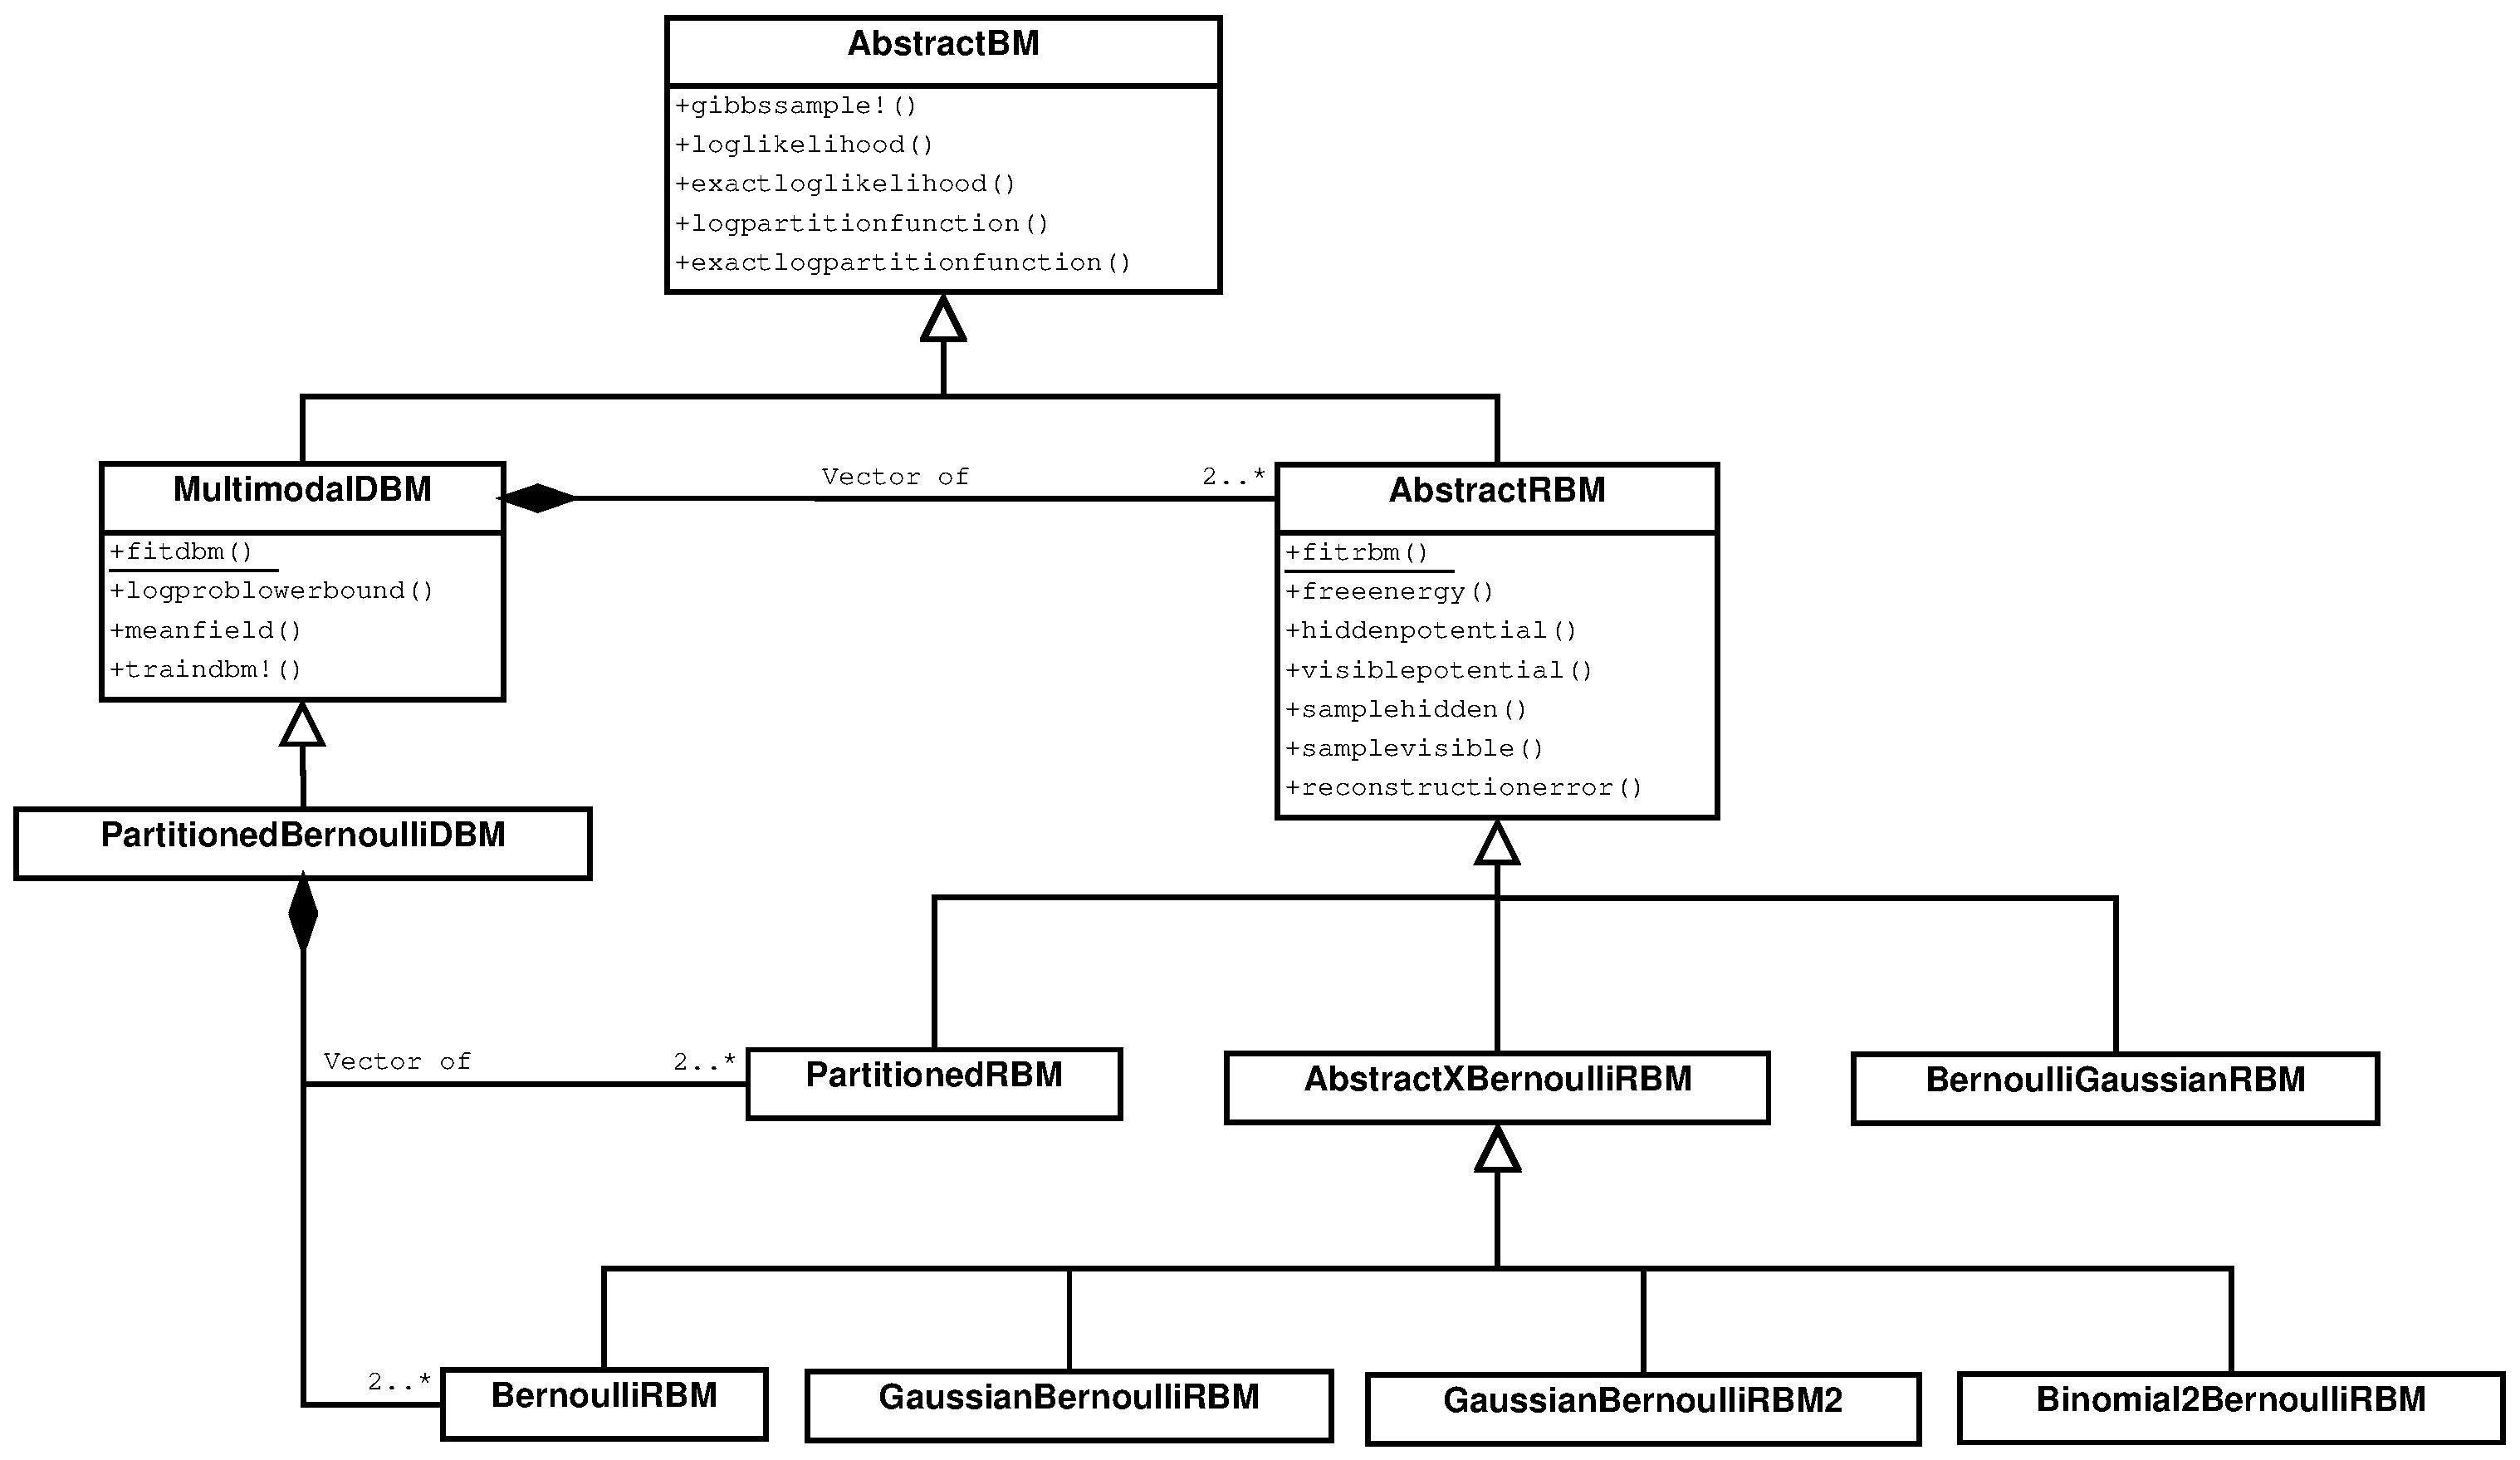
\includegraphics[scale=0.25]{images/BoltzmannMachinesDiagram.eps}
   \caption{UML class diagram \citep{uml} of the type hierarchy for the Boltzmann machines in our Julia implementation. Although the Julia language does not have the concept of classes and visibility, the diagram is suited well to show the connections of the types with the most important associated functions.
   For more details on these functions, see tables \ref{juliaFunTableTrain} and \ref{juliaFunTableEval}.}
   \label{umlclassdiagram}
\end{figure}

\begin{figure}[h]
   \centering
   
\includegraphics[scale=3.]{images/MDBMImpl.eps}
   \caption{Multimodal deep Boltzmann machines are modeled as a stack of restricted Boltzmann machines. On the left hand side an example model is depicted as a graph and on the right hand side the corresponding modelling in the Julia package is shown.
   The first/lowest and the second layer are modelled as a \inlinecode{PartitionedRBM}s (white boxes with grey borders), each containing a vector holding two \inlinecode{BernoulliRBM}s (grey filled boxes).
   The third/highest layer is simply a \inlinecode{BernoulliRBM}.
   All three \inlinecode{AbstractRBMs} in a vector form the \inlinecode{MultimodalDBM}.
   The arrows indicate the ordering of the vectors.}
\label{mdbmimplasstack}
\end{figure}


\rowcolors{1}{gray!25}{white} % alternating row colors in tables
\begin{table}
\begin{tabularx}{\textwidth}{X}
   \hline
   \inlinecode{fitrbm(x;...)} \\
   Fits a restricted Boltzmann machine model for a given data set \inlinecode{x} and additional model hyperparameters \\
   \inlinecode{fitdbm(x; ...)} \\
   Fits a (multimodal) deep Boltzmann machine model for a given data set \inlinecode{x} and model hyperparameters \\
   \inlinecode{meanfield(dbm, x)} \\
   Calculates the mean-field activations of the \inlinecode{dbm}'s hidden nodes given the activations of the visible nodes \inlinecode{x}. \\
   \inlinecode{stackrbms(x;...)} \\
   Pre-trains a stack of RBMs on a given data set \inlinecode{x}. It can either be used for pre-training of a DBM or to train a deep belief network. \\
   \hline
\end{tabularx}
\caption{Functions in the Julia package for training}\label{juliaFunTableTrain}
\end{table}

\rowcolors{1}{gray!25}{white}
\begin{table}
   \begin{tabularx}{\textwidth}{X}
   \hline
   \inlinecode{logpartitionfunction(bm; ... )} \\
   Estimates log of the partition function of the Boltzmann machine \inlinecode{bm} using AIS. Additional hyperparameters for AIS may be provided. \\
   \makecell[tl]{
      \inlinecode{loglikelihood(rbm, x)} \\
      \inlinecode{loglikelihood(rbm, x, logz)}
   } \\
   Calculates the log-likelihood of data \inlinecode{x} in the restricted Boltzmann machine model \inlinecode{rbm}. The log of the partition function can be provided as parameter \inlinecode{logz} or is estimated using AIS. \\
   \makecell[tl]{
      \inlinecode{loglikelihood(dbm, x; ...)} \\
      \inlinecode{loglikelihood(dbm, x, logz; ...)}
   } \\
   Estimates the log-likelihood of a (multimodal) deep Boltzmann machine using AIS for each sample. Additional hyperparameters for AIS may be provided. \\
   \inlinecode{logproblowerbound(dbm, x; ...)} \\
   Estimates the stochastic lower bound of the log-likelihood that is optimized by the training algorithm with mean-field optimization. \\
   \inlinecode{exactloglikelihood(bm, x)} \\
   Calculates the log-likelihood of a deep Boltzmann machine. \\
   \inlinecode{exactlogpartitionfunction(bm, x)} \\
   Calculates the log of the partition function for a restricted Boltzmann machine. \\
   \hline
\end{tabularx}
\caption{Functions in the Julia package for evaluating the likelihood of trained models. The exact calculations of the partition function and the likelihood are only feasible for very small models. For the complexity of the corresponding algorithms, see \ref{methodExactloglik}.}
\label{juliaFunTableEval}
\end{table}

\subsubsection{Training algorithm and choices of hyperparameters}

The hyperparameters for layerwise pre-training can be defined for the whole network or for each layer separately. TODO Trainlayer, AbstractTrainLayer.


\subsubsection{Implementation of annealed importance sampling}

TODO cross validation


% TODO softmax0
\subsection{Connecting R and Julia with the JuliaConnectoR}

\begin{table}
\begin{tabular}{lcl}
\hiderowcolors
message & = & '0x01' call \\
	 & $\mid$ &'0x00' element \\
	 & $\mid$ &'0x50' output \\
	 & $\mid$ &'0x5e' output \\
	 & $\mid$ &'0xff' fail \\
	 & $\mid$ &byebye \\
call & = & string list \\
list & = & int32 \{element\} int32 \{named\_element\} attributes \\
attributes & = & nattributes \{named\_element\} \\
nattributes & = & uint8 \\
named\_element & = & string element \\
element & = & '0x00' \\
		& $\mid$ &'0x01' dimensions \{double\} attributes \\
		& $\mid$ &'0x02' dimensions \{complex\} attributes \\
		& $\mid$ &'0x03' dimensions \{raw\} attributes \\
		& $\mid$ &'0x04' dimensions \{integer\} attributes \\
		& $\mid$ &'0x05' dimensions \{boolean\} \\
		& $\mid$ &'0x06' dimensions \{string\} attributes \\
		& $\mid$ &'0x07' list \\
		& $\mid$ &'0x5b' string (* name of symbol *) \\
		& $\mid$ &'0x5e' object\_class\_id object\_reference \\
		& $\mid$ &'0xcb' callback \\
		& $\mid$ &'0xee' expression \\
		& $\mid$ &'0xfc' named\_function \\
object\_class\_id & = & '0x5c' (* class JuliaStructProxy *) \\
				& $\mid$ &'0x5a' (* class JuliaSimpleArrayProxy *) \\
				& $\mid$ &'0xaf' (* anonymous function reference *) \\
				& $\mid$ &'0xaa' (* class JuliaArrayProxy *) \\
				& $\mid$ &'0x00' (* no information *) \\
object\_reference & = & 8 * byte \\
anonymous\_function\_reference & = & 8 * byte \\
callback & = & string \\
named\_function & = & string \\
string & = & int32 utf8string \\
dimensions & = & ndimensions \{int32\} \\
ndimensions & = & int32 \\
output & = & int32 \{byte\} \\
fail & = & string \\
byebye & = & '0xbb' \\
\end{tabular}
\caption{Serialization grammar for the \apkg{JuliaConnectoR}. TODO: Tabelle aufteilen und erklären}
\end{table}

TODO EBNF syntax \citep{ebnf} für die Grammatik erklären

The grammar is inspired by BSON \citep{bsonspec}.

TODO Rest aus JuliaConnectoR-Paper hier einarbeiten


%* A string is preceded by the number of bytes to UTF-8-encode the string.
%* The sequence of unnamed/positional elements in a list is preceded by
%  the number of (named) elements that follow.
%* Standard output (after '0x50') or standard error output (after '0x5e')
%  is preceded by the number of bytes that are sent.


\subsection{Privacy-preserving deep learning with DataSHIELD}
\begin{figure}[h]
   \centering
   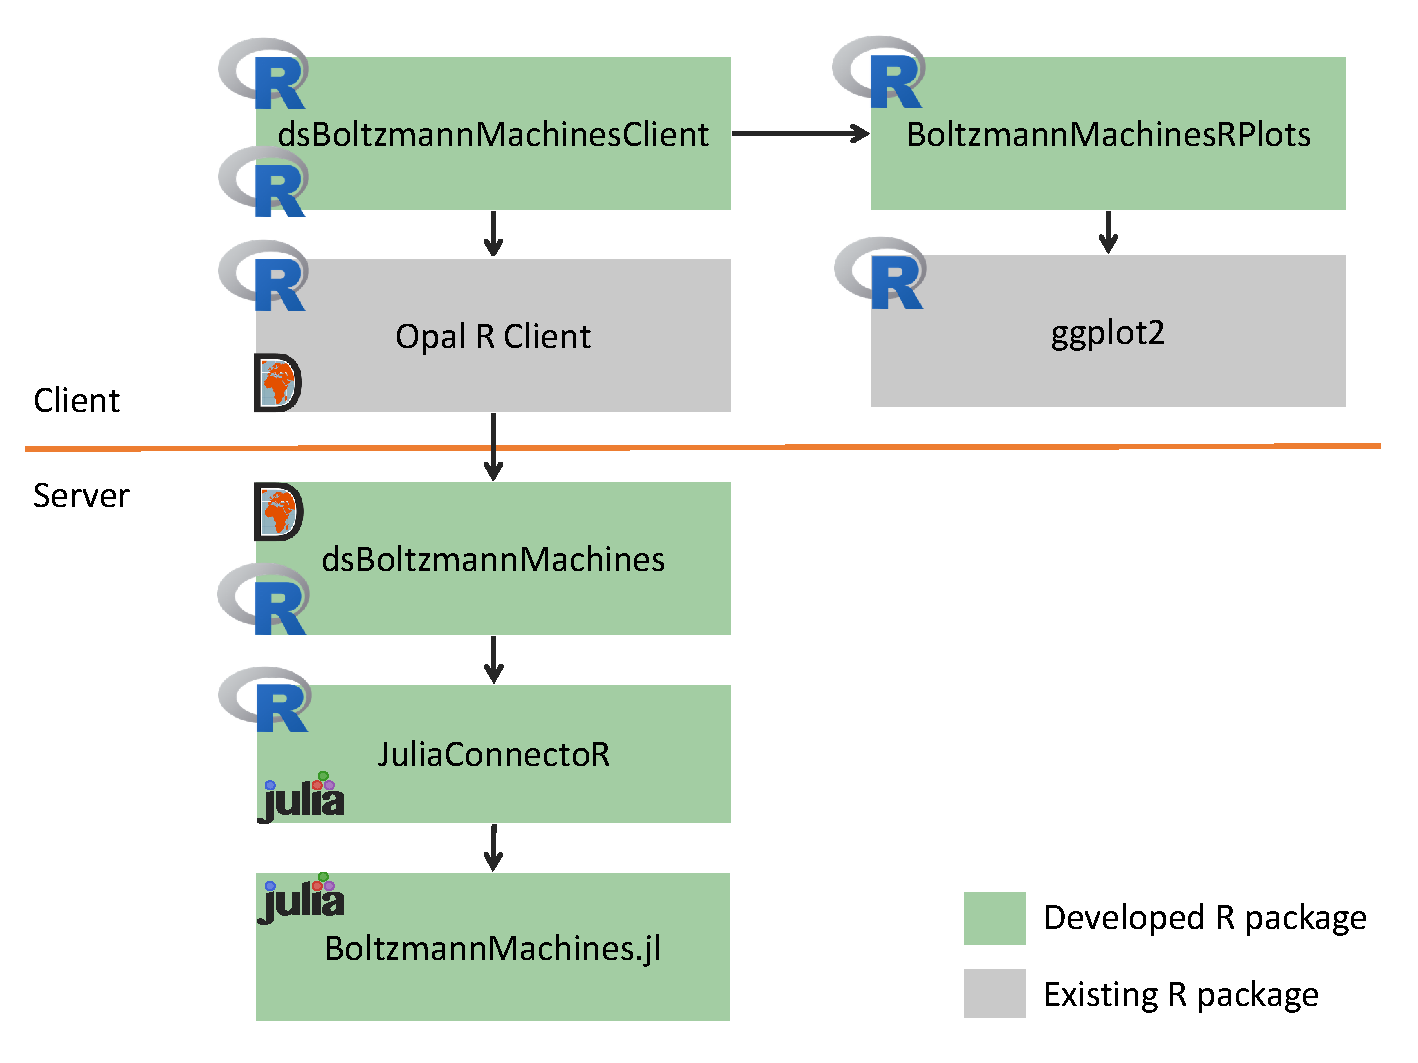
\includegraphics[scale=0.5]{images/dsBoltzmannMachinesOverview.pdf}
   \caption{Overview of dependencies between the developed packages}
 \end{figure}
 
 
\begin{figure}[h]
   \centering
   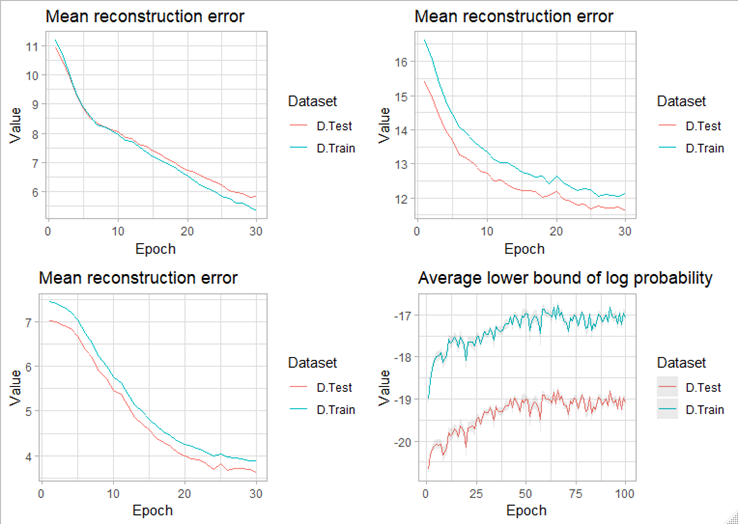
\includegraphics[scale=0.4,trim={0.1cm 0 0 0.1cm},clip]{images/dsBoltzmannLearningcurves.png}
   \caption{Examples for learning curves produced by the package \apkg{BoltzmannMachinesPlots}. This shows learning curves for the training of a DBM with three layers. The plots showing the mean reconstruction error are the result of monitoring the greedy layerwise pre-training. The plot showing the lower bound of the log probability comes is the monitoring output of the fine-tuning of the DBM. There are two curves in each plot, one for the training data and one for the test data.}
 \end{figure}

\begin{figure}[h]
   \centering
   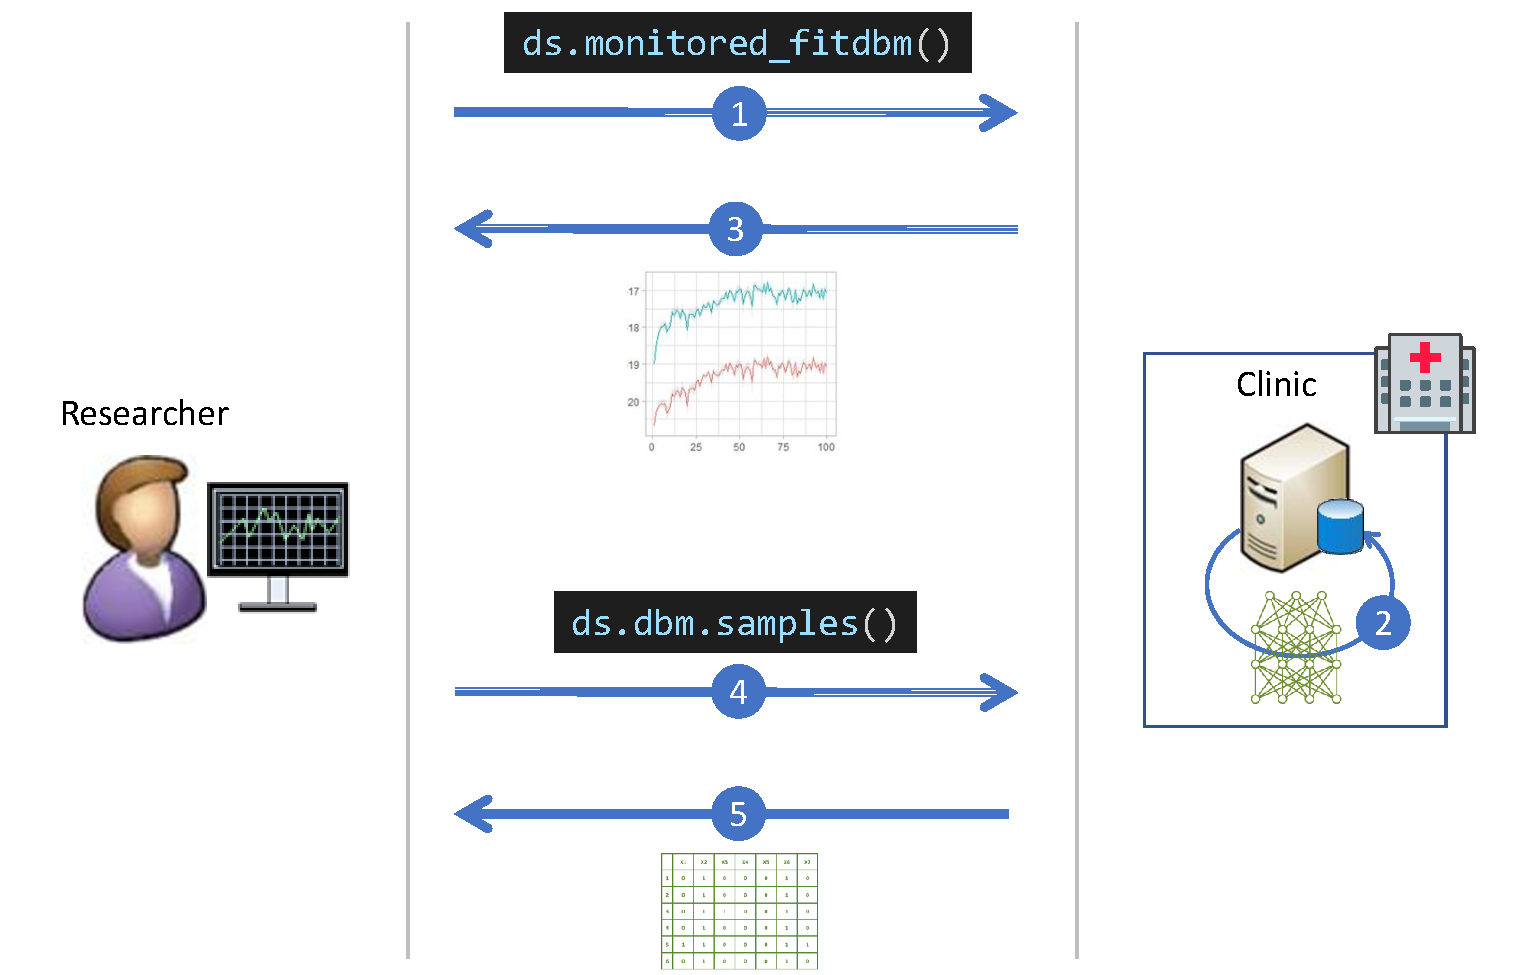
\includegraphics[scale=0.5]{images/dsBoltzmannWorkflow.pdf}
   \caption{Exemplary workflow for using the \apkg{dsBoltzmannMachines} package}
 \end{figure}
 
\clearpage
\FloatBarrier

\section{Discussion}
\subsection{Comparison to other approaches for privacy-preserving deep learning}
TODO
\subsection{Ideas for future work}
% TODO supergenerator
% TODO softmax



\clearpage
\appendix



\begin{appendices}
\section{References}
\renewcommand{\bibsection}{} % funzt nur mit natbib: https://tex.stackexchange.com/a/370784/206178

\bibliography{references}

\clearpage
\section{Publications}
Parts of this work have been published in the following articles:


Basis for this was the work on the package BoltzmannMachines (see Appendix \ref{declcontr})

\section{Declaration of own contributions}\label{declcontr}

The contributions to the published packages and corresponding publications are as follows:

\begin{itemize}
\item 
\end{itemize}

\clearpage
\section[Documentation of Julia package \apkg{BoltzmannMachines}]{Documentation of Julia package \\ \apkg{BoltzmannMachines}}

This appendix lists the documentation for all exported and documented items of the \apkg{BoltzmannMachines} Julia package, as of version 1.2.0. The code of the package and more documentation can be found on the GitHub repository \url{https://github.com/stefan-m-lenz/BoltzmannMachines.jl}.

\subsection*{AbstractOptimizer}
The \texttt{AbstractOptimizer} interface allows to specify optimization procedures. It consists of three methods:

\begin{itemize}
\item \texttt{initialized(optimizer, bm)}: May be used for creating an optimizer that is  specifically initialized for the Boltzmann machine \texttt{bm}.  In particular it may be used to allocate reusable space for the gradient.  The default implementation simply returns the unmodified \texttt{optimizer}.


\item \texttt{computegradient!(optimizer, v, vmodel, h, hmodel, rbm)} or \texttt{computegradient!(optimizer, meanfieldparticles, gibbsparticles, dbm)}  needs to be implemented for computing the gradient given the samples  from the positive and negative phase.


\item \texttt{updateparameters!(bm, optimizer)} needs to be specified for taking the  gradient step. The default implementation for RBMs expects the fields  \texttt{learningrate} and \texttt{gradient} and adds \texttt{learningrate * gradient} to the  given RBM.

\end{itemize}
\noindent\rule{\textwidth}{1pt}
%======================================================
\subsection*{AbstractRBM}
Abstract supertype for all RBMs 

\noindent\rule{\textwidth}{1pt}
%======================================================
\subsection*{AbstractTrainLayer}
Abstract supertype for layerwise training specification. May be specifications for a normal RBM layer (see \texttt{TrainLayer}) or multiple combined specifications for a partitioned layer (see \texttt{TrainPartitionedLayer}).

\noindent\rule{\textwidth}{1pt}
%======================================================
\subsection*{BernoulliGaussianRBM}
\begin{verbatim}
BernoulliGaussianRBM(weights, visbias, hidbias)
\end{verbatim}
Encapsulates the parameters of an RBM with Bernoulli distributed visible nodes and Gaussian distributed hidden nodes. The standard deviation of the Gaussian distribution is 1.

\noindent\rule{\textwidth}{1pt}
%======================================================
\subsection*{BernoulliRBM}
\begin{verbatim}
BernoulliRBM(weights, visbias, hidbias)
\end{verbatim}
Encapsulates the parameters of an RBM with Bernoulli distributed nodes.

\begin{itemize}
\item \texttt{weights}: matrix of weights with size (number of visible nodes, number of hidden nodes)


\item \texttt{visbias}: bias vector for visible nodes


\item \texttt{hidbias}: bias vector for hidden nodes

\end{itemize}
\noindent\rule{\textwidth}{1pt}
%======================================================
\subsection*{Binomial2BernoulliRBM}
\begin{verbatim}
Binomial2BernoulliRBM(weights, visbias, hidbias)
\end{verbatim}
Encapsulates the parameters of an RBM with 0/1/2-valued, Binomial (n=2) distributed visible nodes, and Bernoulli distributed hidden nodes. This model is equivalent to a BernoulliRBM in which every two visible nodes are connected with the same weights to each hidden node. The states (0,0) / (1,0) / (0,1) / (1,1) of the visible nodes connected with with the same weights translate as states 0 / 1 / 1 / 2 in the Binomial2BernoulliRBM.

\noindent\rule{\textwidth}{1pt}
%======================================================
\subsection*{DataDict}
A dictionary containing names of data sets as keys and the data sets (matrices with samples in rows) as values.

\noindent\rule{\textwidth}{1pt}
%======================================================
\subsection*{GaussianBernoulliRBM}
\begin{verbatim}
GaussianBernoulliRBM(weights, visbias, hidbias, sd)
\end{verbatim}
Encapsulates the parameters of an RBM with Gaussian distributed visible nodes and Bernoulli distributed hidden nodes.

\noindent\rule{\textwidth}{1pt}
%======================================================
\subsection*{GaussianBernoulliRBM2}
\begin{verbatim}
GaussianBernoulliRBM2(weights, visbias, hidbias, sd)
\end{verbatim}
Encapsulates the parameters of an RBM with Gaussian distributed visible nodes and Bernoulli distributed hidden nodes with the alternative energy formula proposed by KyungHyun Cho.

\noindent\rule{\textwidth}{1pt}
%======================================================
\subsection*{LoglikelihoodOptimizer}
Implements the \texttt{AbstractOptimizer} interface for optimizing the loglikelihood with stochastic gradient descent.

\noindent\rule{\textwidth}{1pt}
%======================================================
\subsection*{Monitor}
A vector for collecting \texttt{MonitoringItem}s during training.

\noindent\rule{\textwidth}{1pt}
%======================================================
\subsection*{MonitoringItem}
Encapsulates the value of an evaluation calculated in one training epoch. If the evaluation depends on a dataset, the dataset's name can be specified also.

\noindent\rule{\textwidth}{1pt}
%======================================================
\subsection*{Particles}
\texttt{Particles} are an array of matrices. The i'th matrix contains in each row the vector of states of the nodes of the i'th layer of an RBM or a DBM. The set of rows with the same index define an activation state in a Boltzmann Machine. Therefore, the size of the i'th matrix is (number of samples/particles, number of nodes in layer i).

\noindent\rule{\textwidth}{1pt}
%======================================================
\subsection*{PartitionedRBM}
\begin{verbatim}
PartitionedRBM(rbms)
\end{verbatim}
Encapsulates several (parallel) AbstractRBMs that form one partitioned RBM. The nodes of the parallel RBMs are not connected between the RBMs.

\noindent\rule{\textwidth}{1pt}
%======================================================
\subsection*{TrainLayer}
Specify parameters for training one RBM-layer in a DBM.

\paragraph*{Optional keyword arguments:}
\begin{itemize}
\item The optional keyword arguments \texttt{rbmtype}, \texttt{nhidden}, \texttt{epochs}, \texttt{learningrate}/\texttt{learningrates}, \texttt{sdlearningrate}/\texttt{sdlearningrates}, \texttt{categories}, \texttt{batchsize}, \texttt{pcd}, \texttt{cdsteps}, \texttt{startrbm} and \texttt{optimizer}/\texttt{optimizers} are passed to \texttt{fitrbm}. For a detailed description, see there. If a negative value is specified for \texttt{learningrate} or \texttt{epochs}, this indicates that a corresponding default value should be used (parameter defined by call to \texttt{stackrbms}).


\item \texttt{monitoring}: also like in \texttt{fitrbm}, but may take a \texttt{DataDict} as third argument  (see function \texttt{stackrbms} and its argument \texttt{monitoringdata}).


\item \texttt{nvisible}: Number of visible units in the RBM. Only relevant for partitioning.  This parameter is derived as much as possible by \texttt{stackrbms}.  For \texttt{MultimodalDBM}s with a partitioned first layer, it is necessary to specify  the number of visible nodes for all but at most one partition in the input layer.

\end{itemize}
\noindent\rule{\textwidth}{1pt}
%======================================================
\subsection*{TrainPartitionedLayer}
Encapsulates a vector of \texttt{TrainLayer} objects for training a partitioned layer.

\noindent\rule{\textwidth}{1pt}
%======================================================
\subsection*{aislogimpweights}
\begin{verbatim}
aislogimpweights(rbm; ...)
\end{verbatim}
Computes the logarithmised importance weights for estimating the ratio of the partition functions of the given \texttt{rbm} to the RBM with zero weights, but same visible and hidden bias as the \texttt{rbm}. This function implements the Annealed Importance Sampling algorithm (AIS) like described in section 4.1.3 of [Salakhutdinov, 2008].

\paragraph*{Optional keyword arguments (for all types of Boltzmann Machines):}
\begin{itemize}
\item \texttt{ntemperatures}: Number of temperatures for annealing from the starting model to the target model, defaults to 100


\item \texttt{temperatures}: Vector of temperatures. By default \texttt{ntemperatures} ascending numbers, equally spaced from 0.0 to 1.0


\item \texttt{nparticles}: Number of parallel chains and calculated weights, defaults to  100


\item \texttt{burnin}: Number of steps to sample for the Gibbs transition between models

\end{itemize}
\begin{verbatim}
aislogimpweights(rbm1, rbm2; ...)
\end{verbatim}
Computes the logarithmised importance weights for estimating the log-ratio log(Z2/Z1) for the partition functions Z1 and Z2 of \texttt{rbm1} and \texttt{rbm2}, respectively. Implements the procedure described in section 4.1.2 of [Salakhutdinov, 2008]. This requires that \texttt{rbm1} and \texttt{rbm2} are of the same type and have the same number of visible units.

\begin{verbatim}
aislogimpweights(dbm; ...)
\end{verbatim}
Computes the logarithmised importance weights in the Annealed Importance Sampling algorithm (AIS) for estimating the ratio of the partition functions of the given DBM \texttt{dbm} to the base-rate DBM with all weights being zero and all biases equal to the biases of the \texttt{dbm}.

Implements algorithm 4 in [Salakhutdinov+Hinton, 2012]. For DBMs with Bernoulli-distributed nodes only (i. e. here DBMs of type \texttt{PartitionedBernoulliDBM}), it is possible to calculate the importance weights by summing out either the even layers (h1, h3, ...) or the odd layers (v, h2, h4, ...). In the first case, the nodes' activations in the odd layers are used to calculate the probability ratios, in the second case the even layer are used. If \texttt{dbm} is of type \texttt{PartitionedBernoulliDBM}, the optional keyword argument \texttt{sumout} can be used to choose by specifying the values \texttt{:odd} (default) or \texttt{:even}. In the case of \texttt{MultimodalDBM}s, it is not possible to choose and the second case applies there.

\noindent\rule{\textwidth}{1pt}
%======================================================
\subsection*{aisprecision}
\begin{verbatim}
aisprecision(logr, aissd, sdrange)
\end{verbatim}
Returns the differences of the estimated logratio \texttt{r} to the lower and upper bound of the range defined by the multiple \texttt{sdrange} of the standard deviation of the ratio's estimator \texttt{aissd}.

\begin{verbatim}
aisprecision(logimpweights, sdrange)
\end{verbatim}
\noindent\rule{\textwidth}{1pt}
%======================================================
\subsection*{aisstandarddeviation}
Computes the standard deviation of the AIS estimator (not logarithmised) (eq 4.10 in [Salakhutdinov+Hinton, 2012]) given the logarithmised importance weights.

\noindent\rule{\textwidth}{1pt}
%======================================================
\subsection*{barsandstripes}
\begin{verbatim}
barsandstripes(nsamples, nvariables)
\end{verbatim}
Generates a test data set. To see the structure in the data set, run e. g. \texttt{reshape(barsandstripes(1, 16), 4, 4)} a few times.

Example from: MacKay, D. (2003). Information Theory, Inference, and Learning Algorithms

\noindent\rule{\textwidth}{1pt}
%======================================================
\subsection*{computegradient!}
\begin{verbatim}
computegradient!(optimizer, v, vmodel, h, hmodel, rbm)
\end{verbatim}
Computes the gradient of the RBM \texttt{rbm} given the the hidden activation \texttt{h} induced by the sample \texttt{v} and the vectors \texttt{vmodel} and \texttt{hmodel} generated by sampling from the model. The result is stored in the \texttt{optimizer} in such a way that it can be applied by a call to \texttt{updateparameters!}. There is no return value.

For RBMs (excluding PartitionedRBMs), this means saving the gradient in a RBM of the same type in the field \texttt{optimizer.gradient}.

\noindent\rule{\textwidth}{1pt}
%======================================================
\subsection*{crossvalidation}
\begin{verbatim}
crossvalidation(x, monitoredfit; ...)
\end{verbatim}
Performs k-fold cross-validation, given

\begin{itemize}
\item the data set \texttt{x} and


\item \texttt{monitoredfit}: a function that fits and evaluates a model. As arguments it must accept:

\begin{itemize}
\item a training data data set


\item a \texttt{DataDict} containing the evaluation data.

\end{itemize}
\end{itemize}
The return values of the calls to the \texttt{monitoredfit} function are concatenated with \texttt{vcat}. If the monitoredfit function returns \texttt{Monitor} objects, \texttt{crossvalidation} returns a combined \texttt{Monitor} object that can be displayed by creating a cross-validation plot via \texttt{BoltzmannMachinesPlots.crossvalidationplot}.

\paragraph*{Optional named argument:}
\begin{itemize}
\item \texttt{kfold}: specifies the \texttt{k} in "\texttt{k}-fold" (defaults to 10).

crossvalidation(x, monitoredfit, pars; ...)

\end{itemize}
If additionaly a vector of parameters \texttt{pars} is given, \texttt{monitoredfit} also expects an additional parameter from the parameter set.

\noindent\rule{\textwidth}{1pt}
%======================================================
\subsection*{empiricalloglikelihood}
\begin{verbatim}
empiricalloglikelihood(x, xgen)
empiricalloglikelihood(bm, x, nparticles)
empiricalloglikelihood(bm, x, nparticles, burnin)
\end{verbatim}
Computes the mean empirical loglikelihood for the data set \texttt{x}. The probability of a sample is estimated to be the empirical probability of the sample in a dataset generated by the model. This data set can be given as \texttt{xgen} or it is generated by running a Gibbs sampler with \texttt{nparticles} for \texttt{burnin} steps (default 5) in the Boltzmann Machine \texttt{bm}. Throws an error if a sample in \texttt{x} is not contained in the generated data set.

\noindent\rule{\textwidth}{1pt}
%======================================================
\subsection*{energy}
\begin{verbatim}
energy(rbm, v, h)
\end{verbatim}
Computes the energy of the configuration of the visible nodes \texttt{v} and the hidden nodes \texttt{h}, specified as vectors, in the \texttt{rbm}.

\noindent\rule{\textwidth}{1pt}
%======================================================
\subsection*{exactloglikelihood}
\begin{verbatim}
exactloglikelihood(rbm, x)
\end{verbatim}
Computes the mean log-likelihood for the given dataset \texttt{x} and the RBM \texttt{rbm} exactly. The log of the partition function is computed exactly by \texttt{exactlogpartitionfunction(rbm)}. Besides that, the function simply calls \texttt{loglikelihood(rbm, x)}.

\begin{verbatim}
exactloglikelihood(dbm, x)
exactloglikelihood(dbm, x, logz)
\end{verbatim}
Computes the mean log-likelihood for the given dataset \texttt{x} and the DBM \texttt{dbm} exactly. If the value of the log of the partition function of the \texttt{dbm} is not supplied as argument \texttt{logz}, it will be computed by \texttt{exactlogpartitionfunction(dbm)}.

\noindent\rule{\textwidth}{1pt}
%======================================================
\subsection*{exactlogpartitionfunction}
\begin{verbatim}
exactlogpartitionfunction(rbm)
\end{verbatim}
Calculates the log of the partition function of the BernoulliRBM \texttt{rbm} exactly. The execution time grows exponentially with the minimum of (number of visible nodes, number of hidden nodes).

\begin{verbatim}
exactlogpartitionfunction(gbrbm)
\end{verbatim}
Calculates the log of the partition function of the GaussianBernoulliRBM \texttt{gbrbm} exactly. The execution time grows exponentially with the number of hidden nodes.

\begin{verbatim}
exactlogpartitionfunction(bgrbm)
\end{verbatim}
Calculates the log of the partition function of the BernoulliGaussianRBM \texttt{bgrbm} exactly. The execution time grows exponentially with the number of visible nodes.

\begin{verbatim}
exactlogpartitionfunction(dbm)
\end{verbatim}
Calculates the log of the partition function of the DBM \texttt{dbm} exactly. If the number of hidden layers is even, the execution time grows exponentially with the total number of nodes in hidden layers with odd indexes (i. e. h1, h3, ...). If the number of hidden layers is odd, the execution time grows exponentially with the minimum of (number of nodes in layers with even index, number of nodes in layers with odd index).

\begin{verbatim}
exactlogpartitionfunction(mdbm)
\end{verbatim}
Calculates the log of the partition function of the MultimodalDBM \texttt{mdbm} exactly. The execution time grows exponentially with the total number of nodes in hidden layers with odd indexes (i. e. h1, h3, ...).

\noindent\rule{\textwidth}{1pt}
%======================================================
\subsection*{fitdbm}
\begin{verbatim}
fitdbm(x; ...)
\end{verbatim}
Fits a (multimodal) DBM to the data set \texttt{x}. The procedure consists of two parts: First a stack of RBMs is pretrained in a greedy layerwise manner (see \texttt{stackrbms(x)}). Then the weights of all layers are jointly trained using the general Boltzmann Machine learning procedure (see \texttt{traindbm!(dbm,x)}).

\paragraph*{Optional keyword arguments (ordered by importance):}
\begin{itemize}
\item \texttt{nhiddens}: vector that defines the number of nodes in the hidden layers of  the DBM. The default value specifies two hidden layers with the same size  as the visible layer.


\item \texttt{epochs}: number of training epochs for joint training, defaults to 10


\item \texttt{epochspretraining}: number of training epochs for pretraining,  defaults to \texttt{epochs}


\item \texttt{learningrate}/\texttt{learningrates}:  learning rate(s) for joint training of layers (= fine tuning)  using the learning algorithm for a general Boltzmann Machine.  The learning rate for fine tuning is by default decaying with the number of epochs,  starting with the given value for the \texttt{learningrate}.  (For more details see \texttt{traindbm!}).


\item \texttt{learningratepretraining}: learning rate for pretraining,  defaults to \texttt{learningrate}


\item \texttt{batchsizepretraining}: batchsize for pretraining, defaults to 1


\item \texttt{nparticles}: number of particles used for sampling during joint training of  DBM, default 100


\item \texttt{pretraining}: The arguments for layerwise pretraining  can be specified for each layer individually.  This is done via a vector of \texttt{TrainLayer} objects.  (For a detailed description of the possible parameters,  see help for \texttt{TrainLayer}).  If the number of training epochs and the learning rate are not specified  explicitly for a layer, the values of \texttt{epochspretraining},  \texttt{learningratepretraining} and \texttt{batchsizepretraining} are used.


\item \texttt{monitoring}: Monitoring function accepting a \texttt{dbm} and the number of epochs,  returning nothing. Used for the monitoring of fine-tuning.  See also \texttt{monitored\_fitdbm} for a more convenient way of monitoring.


\item \texttt{monitoringdatapretraining}: a \texttt{DataDict} that contains data used for  monitoring the pretraining (see argument \texttt{monitoringdata} of \texttt{stackrbms}.)


\item \texttt{optimizer}/\texttt{optimizers}: an optimizer or a vector of optimizers for each epoch  (see \texttt{AbstractOptimizer}) used for fine-tuning.


\item \texttt{optimizerpretraining}: an optimizer used for pre-training.  Defaults to the \texttt{optimizer}.

\end{itemize}
\noindent\rule{\textwidth}{1pt}
%======================================================
\subsection*{fitrbm}
\begin{verbatim}
fitrbm(x; ...)
\end{verbatim}
Fits an RBM model to the data set \texttt{x}, using Stochastic Gradient Descent (SGD) with Contrastive Divergence (CD), and returns it.

\paragraph*{Optional keyword arguments (ordered by importance):}
\begin{itemize}
\item \texttt{rbmtype}: the type of the RBM that is to be trained  This must be a subtype of \texttt{AbstractRBM} and defaults to \texttt{BernoulliRBM}.


\item \texttt{nhidden}: number of hidden units for the returned RBM


\item \texttt{epochs}: number of training epochs


\item \texttt{learningrate}/\texttt{learningrates}: The learning rate for the weights and biases  can be specified as single value, used throughout all epochs, or as a vector  of \texttt{learningrates} that contains a value for each epoch. Defaults to 0.005.


\item \texttt{batchsize}: number of samples that are used for making one step in the  stochastic gradient descent optimizer algorithm. Default is 1.


\item \texttt{pcd}: indicating whether Persistent Contrastive Divergence (PCD) is to  be used (true, default) or simple CD that initializes the Gibbs Chain with  the training sample (false)


\item \texttt{cdsteps}: number of Gibbs sampling steps for (persistent)  contrastive divergence, defaults to 1


\item \texttt{monitoring}: a function that is executed after each training epoch.  It takes an RBM and the epoch as arguments.  See also \texttt{monitored\_fitrbm} for another way of monitoring.


\item \texttt{categories}: only relevant if \texttt{rbmtype = Softmax0BernoulliRBM}.  The number of categories as \texttt{Int}, if all variables have the same number  of categories, or as \texttt{Vector\{Int\}} that contains the number of categories  of the i'th categorical variable in the i'th entry.


\item \texttt{upfactor}, \texttt{downfactor}: If this function is used for pretraining a part of  a DBM, it is necessary to multiply the weights of the RBM with factors.


\item \texttt{sdlearningrate}/\texttt{sdlearningrates}: learning rate(s) for the  standard deviation if training a \texttt{GaussianBernoulliRBM} or  \texttt{GaussianBernoulliRBM2}. Ignored for other types of RBMs.  It usually must be much smaller than the learning rates for  the weights. By default it is 0.0, which means that the standard deviation  is not learned.


\item \texttt{startrbm}: start training with the parameters of the given RBM.  If this argument is specified, \texttt{nhidden} and \texttt{rbmtype} are ignored.


\item \texttt{optimizer}/\texttt{optimizers}: an object of type \texttt{AbstractOptimizer} or a vector of  them for each epoch. If specified, the optimization is performed as implemented  by the given optimizer type. By default, the \texttt{LoglikelihoodOptimizer}  with the \texttt{learningrate}/\texttt{learningrates} and \texttt{sdlearningrate}/\texttt{sdlearningrates}  is used. For other types of optimizers, the learning rates must be specified  in the \texttt{optimizer}. For more information on how to write your own optimizer,  see \texttt{AbstractOptimizer}.

\end{itemize}
See also: \texttt{monitored\_fitrbm} for a convenient monitoring of the training.

\noindent\rule{\textwidth}{1pt}
%======================================================
\subsection*{freeenergy}
\begin{verbatim}
freeenergy(rbm, x)
\end{verbatim}
Computes the average free energy of the samples in the dataset \texttt{x} for the AbstractRBM \texttt{rbm}.

\begin{verbatim}
freeenergy(rbm, v)
\end{verbatim}
Computes the free energy of the sample \texttt{v} (a vector) for the \texttt{rbm}.

\noindent\rule{\textwidth}{1pt}
%======================================================
\subsection*{gibbssample!}
\begin{verbatim}
gibbssample!(particles, bm, nsteps)
\end{verbatim}
Performs Gibbs sampling on the \texttt{particles} in the Boltzmann machine model \texttt{bm} for \texttt{nsteps} steps. (See also: \texttt{Particles}.) When sampling in multimodal deep Boltzmann machines, in-between layers are assumed to contain only Bernoulli-distributed nodes.

\noindent\rule{\textwidth}{1pt}
%======================================================
\subsection*{gibbssamplecond!}
\begin{verbatim}
gibbssamplecond!(particles, bm, cond, nsteps)
\end{verbatim}
Conditional Gibbs sampling on the \texttt{particles} in the \texttt{bm} for \texttt{nsteps} Gibbs sampling steps.

The variables that are marked in the indexing vector \texttt{cond} are fixed to the initial values in \texttt{particles} during sampling. This way, conditional sampling is performed on these variables.

See also: \texttt{Particles}, \texttt{initparticles}

\noindent\rule{\textwidth}{1pt}
%======================================================
\subsection*{hiddeninput}
\begin{verbatim}
hiddeninput(rbm, v)
\end{verbatim}
Computes the total input of the hidden units in the AbstractRBM \texttt{rbm}, given the activations of the visible units \texttt{v}. \texttt{v} may be a vector or a matrix that contains the samples in its rows.

\noindent\rule{\textwidth}{1pt}
%======================================================
\subsection*{hiddeninput!}
\begin{verbatim}
hiddeninput!(h, rbm, v)
\end{verbatim}
Like \texttt{hiddeninput}, but stores the returned result in \texttt{h}.

\noindent\rule{\textwidth}{1pt}
%======================================================
\subsection*{hiddenpotential}
\begin{verbatim}
hiddenpotential(rbm, v)
hiddenpotential(rbm, v, factor)
\end{verbatim}
Returns the potential for activations of the hidden nodes in the AbstractRBM \texttt{rbm}, given the activations \texttt{v} of the visible nodes. \texttt{v} may be a vector or a matrix that contains the samples in its rows. The potential is a deterministic value to which sampling can be applied to get the activations. In RBMs with Bernoulli distributed hidden units, the potential of the hidden nodes is the vector of probabilities for them to be turned on.

The total input can be scaled with the \texttt{factor}. This is needed when pretraining the \texttt{rbm} as part of a DBM.

\noindent\rule{\textwidth}{1pt}
%======================================================
\subsection*{hiddenpotential!}
\begin{verbatim}
hiddenpotential!(hh, rbm, vv)
hiddenpotential!(hh, rbm, vv, factor)
\end{verbatim}
Like \texttt{hiddenpotential}, but stores the returned result in \texttt{hh}.

\noindent\rule{\textwidth}{1pt}
%======================================================
\subsection*{initialized}
\begin{verbatim}
initialized(optimizer, rbm)
\end{verbatim}
Returns an \texttt{AbstractOptimizer} similar to the given \texttt{optimizer} that can be used to optimize the \texttt{AbstractRBM} \texttt{rbm}.

\noindent\rule{\textwidth}{1pt}
%======================================================
\subsection*{initparticles}
\begin{verbatim}
initparticles(bm, nparticles; biased = false)
\end{verbatim}
Creates particles for Gibbs sampling in an Boltzmann machine \texttt{bm}. (See also: \texttt{Particles})

For Bernoulli distributed nodes, the particles are initialized with Bernoulli(p) distributed values. If \texttt{biased == false}, p is 0.5, otherwise the results of applying the sigmoid function to the bias values are used as values for the nodes' individual p's.

Gaussian nodes are sampled from a normal distribution if \texttt{biased == false}. If \texttt{biased == true} the mean of the Gaussian distribution is shifted by the bias vector and the standard deviation of the nodes is used for sampling.

\noindent\rule{\textwidth}{1pt}
%======================================================
\subsection*{initrbm}
\begin{verbatim}
initrbm(x, nhidden)
initrbm(x, nhidden, rbmtype)
\end{verbatim}
Creates a RBM with \texttt{nhidden} hidden units and initalizes its weights for training on dataset \texttt{x}. \texttt{rbmtype} can be a subtype of \texttt{AbstractRBM}, default is \texttt{BernoulliRBM}.

\noindent\rule{\textwidth}{1pt}
%======================================================
\subsection*{intensities}
\begin{verbatim}
intensities(x)
intensities(x, q1)
intensities(x, q1, q2)
\end{verbatim}
Performs a linear and monotonous transformation on the data set \texttt{x} to fit it the values into the interval [0.0, 1.0]. For more information see \texttt{intensities\_encode}, \texttt{intensities\_decode}.

\noindent\rule{\textwidth}{1pt}
%======================================================
\subsection*{intensities\_decode}
\begin{verbatim}
intensities_decode(x, its)
\end{verbatim}
Backtransforms the intensity values in the data set \texttt{x} (values in the interval [0.0, 1.0])\texttt{to the range of the original values and returns the new data set or vector. The}its\texttt{argument contains the information about the transformation, as it is returned by}intensities\_encode`.

Note that the range is truncated if the original transformation used other quantiles than 0.0 or 1.0 (minimum and maximum).

\paragraph*{Example:}
\begin{verbatim}
x = randn(5, 4)
xint, its = intensities_encode(x, 0.05)
dbm = fitdbm(xint)
xgen = samples(dbm, 5)
intensities_decode(xgen, its)
\end{verbatim}
\noindent\rule{\textwidth}{1pt}
%======================================================
\subsection*{intensities\_encode}
\begin{verbatim}
intensities_encode(x)
intensities_encode(x, q1)
intensities_encode(x, q1, q2)
\end{verbatim}
Performs a linear and monotonous transformation on the data set \texttt{x} to fit it into the interval [0.0, 1.0]. It returns the transformed data set as a first result and the information to reverse the tranformation as a second result. If you are only interested in the transformed values, you can use the function \texttt{intensities}.

If \texttt{q1} is specified, all values below or equal to the quantile specified  by \texttt{q1} are mapped to 0.0. All values above or equal to the quantile specified by \texttt{q2} are mapped to 1.0. \texttt{q2} defaults to \texttt{1 - q1}.

The quantiles are calculated per column/variable.

See also \texttt{intensities\_decode} for the reverse transformation.

\noindent\rule{\textwidth}{1pt}
%======================================================
\subsection*{joindbms}
\begin{verbatim}
joindbms(dbms)
joindbms(dbms, visibleindexes)
\end{verbatim}
Joins the DBMs given by the vector \texttt{dbms} by joining each layer of RBMs. The weights cross-linking the models are initialized with zeros.

If the vector \texttt{visibleindexes} is specified, it is supposed to contain in the i'th entry an indexing vector that determines the positions in the combined DBM for the visible nodes of the i'th of the \texttt{dbms}. By default the indexes of the visible nodes are assumed to be consecutive.

\noindent\rule{\textwidth}{1pt}
%======================================================
\subsection*{joinrbms}
\begin{verbatim}
joinrbms(rbms)
joinrbms(rbms, visibleindexes)
\end{verbatim}
Joins the given vector of \texttt{rbms} of the same type to form one RBM of this type and returns the joined RBM. The weights cross-linking the models are initialized with zeros.

\noindent\rule{\textwidth}{1pt}
%======================================================
\subsection*{loglikelihood}
\begin{verbatim}
loglikelihood(rbm, x)
loglikelihood(rbm, x, logz)
\end{verbatim}
Computes the average log-likelihood of an RBM on a given dataset \texttt{x}. Uses \texttt{logz} as value for the log of the partition function or estimates the partition function with Annealed Importance Sampling.

\begin{verbatim}
loglikelihood(dbm, x; ...)
\end{verbatim}
Estimates the mean log-likelihood of the DBM on the data set \texttt{x} with Annealed Importance Sampling. This requires a separate run of AIS for each sample.

\noindent\rule{\textwidth}{1pt}
%======================================================
\subsection*{logpartitionfunction}
\begin{verbatim}
logpartitionfunction(bm; ...)
logpartitionfunction(bm, logr)
\end{verbatim}
Calculates or estimates the log of the partition function of the Boltzmann Machine \texttt{bm}.

\texttt{r} is an estimator of the ratio of the \texttt{bm}'s partition function Z to the partition function Z\emph{0 of the reference BM with zero weights but same biases as the given \texttt{bm}. In case of a GaussianBernoulliRBM, the reference model also has the same standard deviation parameter. The estimated partition function of the Boltzmann Machine is Z = r * Z}0 with \texttt{r} being the mean of the importance weights. Therefore, the log of the estimated partition function is log(Z) = log(r) + log(Z\_0)

If the log of \texttt{r} is not given as argument \texttt{logr}, Annealed Importance Sampling (AIS) is performed to get a value for it. In this case, the optional arguments for AIS can be specified (see \texttt{aislogimpweights}), and the optional boolean argument \texttt{parallelized} can be used to turn on batch-parallelized computing of the importance weights.

\noindent\rule{\textwidth}{1pt}
%======================================================
\subsection*{logpartitionfunctionzeroweights}
\begin{verbatim}
logpartitionfunctionzeroweights(bm)
\end{verbatim}
Returns the value of the log of the partition function of the Boltzmann Machine that results when one sets the weights of \texttt{bm} to zero, and leaves the other parameters (biases) unchanged.

\noindent\rule{\textwidth}{1pt}
%======================================================
\subsection*{logproblowerbound}
\begin{verbatim}
logproblowerbound(dbm, x; ...)
logproblowerbound(dbm, x, logimpweights; ...)
logproblowerbound(dbm, x, logz; ...)
\end{verbatim}
Estimates the mean of the variational lower bound for the log probability of the DBM on a given dataset \texttt{x} like described in Equation 38 in [Salakhutdinov, 2015]. The logarithmized partition function can be specified directly as \texttt{logz} or by giving the \texttt{logimpweights} from estimating the partition function with the Annealed Importance Sampling algorithm (AIS). (See \texttt{aislogimpweights}.) If neither \texttt{logimpweights} or \texttt{logz} is given, the partition function will be estimated by AIS with default parameters.

\paragraph*{Optional keyword argument:}
\begin{itemize}
\item The approximate posterior distribution may be given as argument \texttt{mu} or is calculated by the mean-field method.

\end{itemize}
\noindent\rule{\textwidth}{1pt}
%======================================================
\subsection*{meanfield}
\begin{verbatim}
meanfield(dbm, x)
meanfield(dbm, x, eps)
\end{verbatim}
Computes the mean-field approximation for the data set \texttt{x} and returns a matrix of particles for the DBM. The number of particles is equal to the number of samples in \texttt{x}. \texttt{eps} is the convergence criterion for the fix-point iteration, default 0.001. It is assumed that all nodes in in-between-layers are Bernoulli distributed.

\noindent\rule{\textwidth}{1pt}
%======================================================
\subsection*{monitored\_fitdbm}
\begin{verbatim}
monitored_fitdbm(x; ...)
\end{verbatim}
This function performs the same training procedure as \texttt{fitdbm}, but facilitates monitoring: It fits an DBM model on the data set \texttt{x} using greedy layerwise pre-training and subsequent fine-tuning and collects all the monitoring results during the training. The monitoring results are stored in a vector of \texttt{Monitor}s, containing one element for each RBM layer and as last element the monitoring results for fine-tuning. (Monitoring elements from the pre-training of partitioned layers are again vectors, containing one element for each partition.) Both the collected monitoring results and the trained DBM are returned.

See also: \texttt{monitored\_stackrbms}, \texttt{monitored\_traindbm!}

\paragraph*{Optional keyword arguments:}
\begin{itemize}
\item \texttt{monitoring}: Used for fine-tuning. A monitoring function or a vector of monitoring functions that accept four arguments:

\begin{itemize}
\item[1. ] a \texttt{Monitor} object, which is used to collect the result of the monitoring function(s)


\item[2. ] the DBM


\item[3. ] the epoch


\item[4. ] the data used for monitoring.

\end{itemize}
By default, there is no monitoring of fine-tuning.


\item \texttt{monitoringdata}: a \texttt{DataDict}, which contains the data that is used for the  monitoring. For the pre-training of the first layer and for fine-tuning,  the data is passed directly to the \texttt{monitoring} function(s).  For monitoring the pre-training of the higher RBM layers,  the data is propagated through the layers below first.  By default, the training data \texttt{x} is used for monitoring.


\item \texttt{monitoringpretraining}: Used for pre-training. A four-argument function like  \texttt{monitoring}, but accepts as second argument an RBM.  By default there is no monitoring of the pre-training.


\item \texttt{monitoringdatapretraining}: Monitoring data used only for pre-training.  Defaults to \texttt{monitoringdata}.


\item Other specified keyword arguments are simply handed to \texttt{fitdbm}. For more information, please see the documentation there.

\end{itemize}
\paragraph*{Example:}
\begin{verbatim}
using Random; Random.seed!(1)
xtrain, xtest = splitdata(barsandstripes(100, 4), 0.5)
monitors, rbm = monitored_fitdbm(xtrain;
    monitoringpretraining = monitorreconstructionerror!,
    monitoring = monitorlogproblowerbound!,
    monitoringdata = DataDict("Training data" => xtrain, "Test data" => xtest),
    # some arguments for `fitdbm`:
    nhiddens = [4; 3], learningratepretraining = 0.01,
    learningrate = 0.05, epochspretraining = 100, epochs = 50)
using BoltzmannMachinesPlots
plotevaluation(monitors[1]) # view monitoring of first RBM
plotevaluation(monitors[2]) # view monitoring of second RBM
plotevaluation(monitors[3]) # view monitoring fine-tuning
\end{verbatim}
\noindent\rule{\textwidth}{1pt}
%======================================================
\subsection*{monitored\_fitrbm}
\begin{verbatim}
monitored_fitrbm(x; ...)
\end{verbatim}
This function performs the same training procedure as \texttt{fitrbm}, but facilitates monitoring: It fits an RBM model on the data set \texttt{x} and collects monitoring results during the training in one \texttt{Monitor} object. Both the collected monitoring results and the trained RBM are returned.

\paragraph*{Optional keyword arguments:}
\begin{itemize}
\item \texttt{monitoring}: A monitoring function or a vector of monitoring functions that accept four arguments:

\begin{itemize}
\item[1. ] a \texttt{Monitor} object, which is used to collect the result of the monitoring function(s)


\item[2. ] the RBM


\item[3. ] the epoch


\item[4. ] the data used for monitoring.

\end{itemize}
By default, there is no monitoring.


\item \texttt{monitoringdata}: a \texttt{DataDict}, which contains the data that is used for  monitoring and passed to the \texttt{monitoring} functions(s).  By default, the training data \texttt{x} is used for monitoring.


\item Other specified keyword arguments are simply handed to \texttt{fitrbm}. For more information, please see the documentation there.

\end{itemize}
\paragraph*{Example:}
\begin{verbatim}
using Random; Random.seed!(0)
xtrain, xtest = splitdata(barsandstripes(100, 4), 0.3)
monitor, rbm = monitored_fitrbm(xtrain;
    monitoring = [monitorreconstructionerror!, monitorexactloglikelihood!],
    monitoringdata = DataDict("Training data" => xtrain, "Test data" => xtest),
    # some arguments for `fitrbm`:
    nhidden = 10, learningrate = 0.002, epochs = 200)
using BoltzmannMachinesPlots
plotevaluation(monitor, monitorreconstructionerror)
plotevaluation(monitor, monitorexactloglikelihood)
\end{verbatim}
\noindent\rule{\textwidth}{1pt}
%======================================================
\subsection*{monitored\_stackrbms}
\begin{verbatim}
monitored_stackrbms(x; ...)
\end{verbatim}
This function performs the same training procedure as \texttt{stackrbms}, but facilitates monitoring: It trains a stack of RBMs using the data set \texttt{x} as input to the first layer and collects all the monitoring results during the training in a vector of \texttt{Monitor}s, containing one element for each RBM layer. (Elements for partitioned layers are again vectors, containing one element for each partition.) Both the collected monitoring results and the stack of trained RBMs are returned.

\paragraph*{Optional keyword arguments:}
\begin{itemize}
\item \texttt{monitoring}: A monitoring function or a vector of monitoring functions that accept four arguments:

\begin{itemize}
\item[1. ] a \texttt{Monitor} object, which is used to collect the result of the monitoring function(s)


\item[2. ] the RBM


\item[3. ] the epoch


\item[4. ] the data used for monitoring.

\end{itemize}
By default, there is no monitoring.


\item \texttt{monitoringdata}: a \texttt{DataDict}, which contains the data that is used for  monitoring. For the first layer, the data is passed directly to the \texttt{monitoring}  function(s). For monitoring the training of the higher layers,  the data is propagated through the layers below first.  By default, the training data \texttt{x} is used for monitoring.


\item Other specified keyword arguments are simply handed to \texttt{stackrbms}. For more information, please see the documentation there.

\end{itemize}
\paragraph*{Example:}
\begin{verbatim}
using Random; Random.seed!(0)
xtrain, xtest = splitdata(barsandstripes(100, 4), 0.5)
monitors, rbm = monitored_stackrbms(xtrain;
    monitoring = monitorreconstructionerror!,
    monitoringdata = DataDict("Training data" => xtrain, "Test data" => xtest),
    # some arguments for `stackrbms`:
    nhiddens = [4; 3], learningrate = 0.005, epochs = 100)
using BoltzmannMachinesPlots
plotevaluation(monitors[1]) # view monitoring of first RBM
plotevaluation(monitors[2]) # view monitoring of second RBM
\end{verbatim}
\noindent\rule{\textwidth}{1pt}
%======================================================
\subsection*{monitored\_traindbm!}
\begin{verbatim}
monitored_traindbm!(dbm, x; ...)
\end{verbatim}
This function performs the same training procedure as \texttt{traindbm!}, but facilitates monitoring: It performs fine-tuning of the given \texttt{dbm} on the data set \texttt{x} and collects monitoring results during the training in one \texttt{Monitor} object. Both the collected monitoring results and the trained \texttt{dbm} are returned.

\paragraph*{Optional keyword arguments:}
\begin{itemize}
\item \texttt{monitoring}: A monitoring function or a vector of monitoring functions that accept four arguments:

\begin{itemize}
\item[1. ] a \texttt{Monitor} object, which is used to collect the result of the monitoring function(s)


\item[2. ] the DBM


\item[3. ] the epoch


\item[4. ] the data used for monitoring.

\end{itemize}
By default, there is no monitoring.


\item \texttt{monitoringdata}: a \texttt{DataDict}, which contains the data that is used for  monitoring and passed to the \texttt{monitoring} functions(s).  By default, the training data \texttt{x} is used for monitoring.


\item Other specified keyword arguments are simply handed to \texttt{traindbm!}. For more information, please see the documentation there.

\end{itemize}
\paragraph*{Example:}
\begin{verbatim}
using Random; Random.seed!(0)
xtrain, xtest = splitdata(barsandstripes(100, 4), 0.1)
dbm = stackrbms(xtrain; predbm = true, epochs = 20)
monitor, dbm = monitored_traindbm!(dbm, xtrain;
    monitoring = monitorlogproblowerbound!,
    monitoringdata = DataDict("Training data" => xtrain, "Test data" => xtest),
    # some arguments for `traindbm!`:
    epochs = 100, learningrate = 0.1)
using BoltzmannMachinesPlots
plotevaluation(monitor)
\end{verbatim}
\noindent\rule{\textwidth}{1pt}
%======================================================
\subsection*{monitorexactloglikelihood!}
\begin{verbatim}
monitorexactloglikelihood!(monitor, bm, epoch, datadict)
\end{verbatim}
Computes the mean exact log-likelihood in the Boltzmann Machine model \texttt{bm} for the data sets in the DataDict \texttt{datadict} and stores this information in the Monitor \texttt{monitor}.

\noindent\rule{\textwidth}{1pt}
%======================================================
\subsection*{monitorfreeenergy!}
\begin{verbatim}
monitorfreeenergy!(monitor, rbm, epoch, datadict)
\end{verbatim}
Computes the free energy for the \texttt{datadict}'s data sets in the RBM model \texttt{rbm} and stores the information in the \texttt{monitor}.

\noindent\rule{\textwidth}{1pt}
%======================================================
\subsection*{monitorloglikelihood!}
\begin{verbatim}
monitorloglikelihood!(monitor, rbm, epoch, datadict)
\end{verbatim}
Estimates the log-likelihood of the \texttt{datadict}'s data sets in the RBM model \texttt{rbm} with AIS and stores the values, together with information about the variance of the estimator, in the \texttt{monitor}.

If there is more than one worker available, the computation is parallelized by default. Parallelization can be turned on or off with the optional boolean argument \texttt{parallelized}.

For the other optional keyword arguments, see \texttt{aislogimportanceweights}.

See also: \texttt{loglikelihood}.

\noindent\rule{\textwidth}{1pt}
%======================================================
\subsection*{monitorlogproblowerbound!}
\begin{verbatim}
monitorlogproblowerbound!(monitor, dbm, epoch, datadict)
\end{verbatim}
Estimates the lower bound of the log probability of the \texttt{datadict}'s data sets in the DBM \texttt{dbm} with AIS and stores the values, together with information about the variance of the estimator, in the \texttt{monitor}.

If there is more than one worker available, the computation is parallelized by default. Parallelization can be turned on or off with the optional boolean argument \texttt{parallelized}.

For the other optional keyword arguments, see \texttt{aislogimpweights}.

See also: \texttt{logproblowerbound}.

\noindent\rule{\textwidth}{1pt}
%======================================================
\subsection*{monitorreconstructionerror!}
\begin{verbatim}
monitorreconstructionerror!(monitor, rbm, epoch, datadict)
\end{verbatim}
Computes the reconstruction error for the data sets in the \texttt{datadict} and the \texttt{rbm} and stores the values in the \texttt{monitor}.

\noindent\rule{\textwidth}{1pt}
%======================================================
\subsection*{monitorweightsnorm!}
\begin{verbatim}
monitorweightsnorm!(monitor, rbm, epoch)
\end{verbatim}
Computes the L2-norm of the weights matrix and the bias vectors of the \texttt{rbm} and stores the values in the \texttt{monitor}. These values can give a hint how much the updates are changing the parameters during learning.

\noindent\rule{\textwidth}{1pt}
%======================================================
\subsection*{oneornone\_decode}
\begin{verbatim}
oneornone_decode(x, categories)
\end{verbatim}
Returns a dataset such that \texttt{x .== oneornone\_decode(oneornone\_encode(x, categories), categories)}.

For more, see \texttt{oneornone\_encode}.

\noindent\rule{\textwidth}{1pt}
%======================================================
\subsection*{oneornone\_encode}
\begin{verbatim}
oneornone_encode(x, categories)
\end{verbatim}
Expects a data set \texttt{x} containing values 0.0, 1.0, 2.0 ... encoding the categories. Returns a data set that encodes the variables/columns in \texttt{x} in multiple columns with only values 0.0 and 1.0, similiar to the one-hot encoding with the deviation that a zero is encoded as all-zeros.

The \texttt{categories} can be specified as

\begin{itemize}
\item integer number if all variables have the same number of categories or as


\item integer vector, containing for each variable the number of categories encoded.

\end{itemize}
See also \texttt{oneornone\_decode} for the reverse transformation.

\noindent\rule{\textwidth}{1pt}
%======================================================
\subsection*{propagateforward}
\begin{verbatim}
propagateforward(rbm, datadict, factor)
\end{verbatim}
Returns a new \texttt{DataDict} containing the same labels as the given \texttt{datadict} but as mapped values it contains the hidden potential in the \texttt{rbm} of the original datasets. The factor is applied for calculating the hidden potential and is 1.0 by default.

\noindent\rule{\textwidth}{1pt}
%======================================================
\subsection*{reconstructionerror}
\begin{verbatim}
reconstructionerror(rbm, x)
\end{verbatim}
Computes the mean reconstruction error of the RBM on the dataset \texttt{x}.

\noindent\rule{\textwidth}{1pt}
%======================================================
\subsection*{samplehidden}
\begin{verbatim}
samplehidden(rbm, v)
samplehidden(rbm, v, factor)
\end{verbatim}
Returns activations of the hidden nodes in the AbstractRBM \texttt{rbm}, sampled from the state \texttt{v} of the visible nodes. \texttt{v} may be a vector or a matrix that contains the samples in its rows. For the \texttt{factor}, see \texttt{hiddenpotential(rbm, v, factor)}.

\noindent\rule{\textwidth}{1pt}
%======================================================
\subsection*{samplehidden!}
\begin{verbatim}
samplehidden!(h, rbm, v)
samplehidden!(h, rbm, v, factor)
\end{verbatim}
Like \texttt{samplehidden}, but stores the returned result in \texttt{h}.

\noindent\rule{\textwidth}{1pt}
%======================================================
\subsection*{sampleparticles}
\begin{verbatim}
sampleparticles(bm, nparticles, burnin)
\end{verbatim}
Samples in the Boltzmann Machine model \texttt{bm} by running \texttt{nparticles} parallel, randomly initialized Gibbs chains for \texttt{burnin} steps. Returns particles containing \texttt{nparticles} generated samples. See also: \texttt{Particles}.

\noindent\rule{\textwidth}{1pt}
%======================================================
\subsection*{samples}
\begin{verbatim}
samples(bm, nsamples; ...)
\end{verbatim}
Generates \texttt{nsamples} samples from a Boltzmann machine model \texttt{bm} by running a Gibbs sampler. This can also be used for sampling from a \emph{conditional distribution} (see argument \texttt{conditions} below.)

\paragraph*{Optional keyword arguments:}
\begin{itemize}
\item \texttt{burnin}: Number of Gibbs sampling steps, defaults to 50.


\item \texttt{conditions}: \texttt{Vector\{Pair\{Int,Float64\}\}}, containing pairs of variables and their values that are to be conditioned on. E. g. \texttt{[1 => 1.0, 3 => 0.0]}


\item \texttt{samplelast}: boolean to indicate whether to sample in last step (true, default) or whether to use the activation potential.

\end{itemize}
\noindent\rule{\textwidth}{1pt}
%======================================================
\subsection*{samplevisible}
\begin{verbatim}
samplevisible(rbm, h)
samplevisible(rbm, h, factor)
\end{verbatim}
Returns activations of the visible nodes in the AbstractRBM \texttt{rbm}, sampled from the state \texttt{h} of the hidden nodes. \texttt{h} may be a vector or a matrix that contains the samples in its rows. For the \texttt{factor}, see \texttt{visiblepotential(rbm, h, factor)}.

\noindent\rule{\textwidth}{1pt}
%======================================================
\subsection*{samplevisible!}
\begin{verbatim}
samplevisible!(v, rbm, h)
samplevisible!(v, rbm, h, factor)
\end{verbatim}
Like \texttt{samplevisible}, but stores the returned result in \texttt{v}.

\noindent\rule{\textwidth}{1pt}
%======================================================
\subsection*{splitdata}
\begin{verbatim}
splitdata(x, ratio)
\end{verbatim}
Splits the data set \texttt{x} randomly in two data sets \texttt{x1} and \texttt{x2}, such that the fraction of samples in \texttt{x2} is equal to (or as close as possible to) the given \texttt{ratio}.

\paragraph*{Example:}
\begin{verbatim}
trainingdata, testdata = splitdata(data, 0.1) # Use 10 % as test data
\end{verbatim}
\noindent\rule{\textwidth}{1pt}
%======================================================
\subsection*{stackrbms}
\begin{verbatim}
stackrbms(x; ...)
\end{verbatim}
Performs greedy layerwise training for Deep Belief Networks or greedy layerwise pretraining for Deep Boltzmann Machines and returns the trained model.

\paragraph*{Optional keyword arguments (ordered by importance):}
\begin{itemize}
\item \texttt{predbm}: boolean indicating that the greedy layerwise training is  pre-training for a DBM.  If its value is false (default), a DBN is trained.


\item \texttt{nhiddens}: vector containing the number of nodes of the i'th hidden layer in  the i'th entry


\item \texttt{epochs}: number of training epochs


\item \texttt{learningrate}: learningrate, default 0.005


\item \texttt{batchsize}: size of minibatches, defaults to 1


\item \texttt{trainlayers}: a vector of \texttt{TrainLayer} objects. With this argument it is possible  to specify the training parameters for each layer/RBM individually.  If the number of training epochs and the learning rate are not specified  explicitly for a layer, the values of \texttt{epochs} and \texttt{learningrate} are used.  For more information see help of \texttt{TrainLayer}.


\item \texttt{monitoringdata}: a data dictionary (see type \texttt{DataDict})  The data is propagated forward through the  network to monitor higher levels.  If a non-empty dictionary is given, the monitoring functions in the  \texttt{trainlayers}-arguments must accept a \texttt{DataDict} as third argument.


\item \texttt{optimizer}: an optimizer (of type \texttt{AbstractOptimizer}) that is used for  computing the gradients when training the individual RBMs.


\item \texttt{samplehidden}: boolean indicating that consequent layers are to be trained  with sampled values instead of the deterministic potential.  Using the deterministic potential (\texttt{false}) is the default.

\end{itemize}
See also: \texttt{monitored\_stackrbms} for a more convenient monitoring.

\noindent\rule{\textwidth}{1pt}
%======================================================
\subsection*{traindbm!}
\begin{verbatim}
traindbm!(dbm, x; ...)
\end{verbatim}
Trains the \texttt{dbm} (a \texttt{BasicDBM} or a more general \texttt{MultimodalDBM}) using the learning procedure for a general Boltzmann Machine with the training data set \texttt{x}. A learning step consists of mean-field inference (positive phase), stochastic approximation by Gibbs Sampling (negative phase) and the parameter updates.

\paragraph*{Optional keyword arguments (ordered by importance):}
\begin{itemize}
\item \texttt{epoch}: number of training epochs


\item \texttt{learningrate}/\texttt{learningrates}: a vector of learning rates for each epoch to  update the weights and biases. The learning rates should decrease with the  epochs, e. g. with the factor \texttt{a / (b + epoch)}. If only one value is given as  \texttt{learningrate}, \texttt{a} and \texttt{b} are 11.0 and 10.0, respectively.


\item \texttt{nparticles}: number of particles used for sampling, default 100


\item \texttt{monitoring}: A function that is executed after each training epoch.  It has to accept the trained DBM and the current epoch as arguments.

\end{itemize}
\begin{verbatim}
traindbm!(dbm, x, particles, learningrate)
\end{verbatim}
Trains the given \texttt{dbm} for one epoch.

\noindent\rule{\textwidth}{1pt}
%======================================================
\subsection*{trainrbm!}
\begin{verbatim}
trainrbm!(rbm, x)
\end{verbatim}
Trains the given \texttt{rbm} for one epoch using the data set \texttt{x}. (See also function \texttt{fitrbm}.)

\paragraph*{Optional keyword arguments:}
\begin{itemize}
\item \texttt{learningrate}, \texttt{cdsteps}, \texttt{sdlearningrate}, \texttt{upfactor}, \texttt{downfactor},  \texttt{optimizer}:  See documentation of function \texttt{fitrbm}.


\item \texttt{chainstate}: a matrix for holding the states of the RBM's hidden nodes. If  it is specified, PCD is used.

\end{itemize}
\noindent\rule{\textwidth}{1pt}
%======================================================
\subsection*{updateparameters!}
\begin{verbatim}
updateparameters!(rbm, optimizer)
\end{verbatim}
Updates the RBM \texttt{rbm} by walking a step in the direction of the gradient that has been computed by calling \texttt{computegradient!} on \texttt{optimizer}.

\noindent\rule{\textwidth}{1pt}
%======================================================
\subsection*{visibleinput}
\begin{verbatim}
visibleinput(rbm, h)
\end{verbatim}
Returns activations of the visible nodes in the AbstractXBernoulliRBM \texttt{rbm}, sampled from the state \texttt{h} of the hidden nodes. \texttt{h} may be a vector or a matrix that contains the samples in its rows.

\noindent\rule{\textwidth}{1pt}
%======================================================
\subsection*{visibleinput!}
\begin{verbatim}
visibleinput!(v, rbm, h)
\end{verbatim}
Like \texttt{visibleinput} but stores the returned result in \texttt{v}.

\noindent\rule{\textwidth}{1pt}
%======================================================
\subsection*{visiblepotential}
\begin{verbatim}
visiblepotential(rbm, h)
visiblepotential(rbm, h, factor)
\end{verbatim}
Returns the potential for activations of the visible nodes in the AbstractRBM \texttt{rbm}, given the activations \texttt{h} of the hidden nodes. \texttt{h} may be a vector or a matrix that contains the samples in its rows. The potential is a deterministic value to which sampling can be applied to get the activations.

The total input can be scaled with the \texttt{factor}. This is needed when pretraining the \texttt{rbm} as part of a DBM.

In RBMs with Bernoulli distributed visible units, the potential of the visible nodes is the vector of probabilities for them to be turned on.

For a Binomial2BernoulliRBM, the visible units are sampled from a Binomial(2,p) distribution in the Gibbs steps. In this case, the potential is the vector of values for 2p. (The value is doubled to get a value in the same range as the sampled one.)

For GaussianBernoulliRBMs, the potential of the visible nodes is the vector of means of the Gaussian distributions for each node.

\noindent\rule{\textwidth}{1pt}
%======================================================
\subsection*{visiblepotential!}
\begin{verbatim}
visiblepotential!(v, rbm, h)
\end{verbatim}
Like \texttt{visiblepotential} but stores the returned result in \texttt{v}.

\noindent\rule{\textwidth}{1pt}
%======================================================

\clearpage
\section[Documentation of R package \apkg{JuliaConnectoR}]{Documentation of R package \\ \apkg{JuliaConnectoR}}
This appendix lists the documentation for all exported and items of the \apkg{JuliaConnectoR} R package, as of version 0.6.1. The code of the package and more documentation can be found on the GitHub repository \url{https://github.com/stefan-m-lenz/JuliaConnectoR}. The package is also available from the official R CRAN repository: \url{https://CRAN.R-project.org/package=JuliaConnectoR}.

\HeaderA{JuliaConnectoR-package}{A Functionally Oriented Interface for Integrating Julia with R}{JuliaConnectoR.Rdash.package}
%
\begin{Description}\relax
This package provides a functionally oriented interface between R and Julia.
The goal is to call functions from Julia packages directly as R functions.
\end{Description}
%
\begin{Details}\relax
This R-package provides a functionally oriented interface between R and Julia.
The goal is to call functions from Julia packages directly as R functions.
Julia functions imported via the \pkg{JuliaConnectoR} can accept and return R variables.
It is also possible to pass R functions as arguments in place of Julia functions,
which allows \emph{callbacks} from Julia to R.

From a technical perspective, R data structures are serialized with an optimized custom streaming format,
sent to a (local) Julia TCP server, and translated to Julia data structures by Julia.
The results are returned back to R.
Simple objects, which correspond to vectors in R, are directly translated.
Complex Julia structures are by default transferred to R by reference via proxy objects.
This enables an effective and intuitive handling of the Julia objects via R.
It is also possible to fully translate Julia objects to R objects.
These translated objects are annotated with information
about the original Julia objects, such that they can be translated back to Julia.
This makes it also possible to serialize them as R objects.
\end{Details}
%
\begin{Section}{Setup}

The package requires that
\Rhref{https://julialang.org/downloads/}{Julia (Version \eqn{\geq}{} 1.0) is installed}
and that the Julia executable is in the system search \env{PATH} or that the
\env{JULIA\_BINDIR} environment variable is set to the \code{bin} directory of
the Julia installation.
\end{Section}
%
\begin{Section}{Function overview}

The function \code{\LinkA{juliaImport}{juliaImport}} makes
functions and data types from Julia packages or modules available as R functions.

If only a single Julia function needs to be importedR, \code{\LinkA{juliaFun}{juliaFun}}
can do this. The simplest way to call a Julia function without any importing
is to use \code{\LinkA{juliaCall}{juliaCall}} with the function name given
as character string.

For evaluating expressions in Julia, \code{\LinkA{juliaEval}{juliaEval}} and
\code{\LinkA{juliaLet}{juliaLet}} can be used. With \code{\LinkA{juliaLet}{juliaLet}} one can use
R variables in a expression.

\code{\LinkA{juliaExpr}{juliaExpr}} makes it possible use complex Julia syntax in R via R strings
that contain Julia expressions.

With \code{\LinkA{juliaGet}{juliaGet}}, a full translation of a Julia proxy object into an R object
is performed.

\code{as.data.frame} is overloaded (\code{\LinkA{as.data.frame.JuliaProxy}{as.data.frame.JuliaProxy}})
for translating Julia objects that implement the
\Rhref{https://github.com/JuliaData/Tables.jl}{\code{Tables}} interface
to R data frames.
\end{Section}
%
\begin{Section}{Translation}


Since Julia is more type-sensitive than R, and many Julia functions expect to be called
using specific types, it is important to know the translations of the R data structures
to Julia.

%
\begin{SubSection}{Translation from R to Julia}
The type correspondences of the basic R data types in Julia are the following:


\Tabular{lcl}{
\strong{R} &  & \strong{Julia}\\{}
\code{integer} & \eqn{\rightarrow}{} & \code{Int} \\{}
\code{double}  & \eqn{\rightarrow}{} & \code{Float64} \\{}
\code{logical}   & \eqn{\rightarrow}{} & \code{Bool} \\{}
\code{character} & \eqn{\rightarrow}{} & \code{String} \\{}
\code{complex} & \eqn{\rightarrow}{} & \code{Complex\{Float64\}} \\{}
\code{raw}  & \eqn{\rightarrow}{} & \code{UInt8} \\{}
\code{symbol} & \eqn{\rightarrow}{} & \code{Symbol}
}

R vectors of length 1 of the types in the table above will be translated to the types shown.

R vectors or arrays with more than one element will be translated to Julia \code{Array}s
of the corresponding types. The dimensions of an R array, as returned by \code{dim()},
will also be respected.
For example, the R integer vector \code{c(1L, 2L)} will be of type \code{Vector\{Int\}},
or \code{Array\{Int,1\}}, in Julia.
A double matrix such as \code{matrix(c(1,2,3,4), nrow = 2)}
will be of type \code{Array\{Float64,2\}}.

Missing values (\code{NA}) in R are translated to \code{missing} values in Julia.
R vectors and arrays with missing values are converted to Julia arrays
of type \code{Array\{Union\{Missing, T\}\}}, where \code{T} stands for the translated 
type in the table above.

R lists are translated as \code{Vector\{T\}} in Julia, with \code{T} being
the most specific supertype of the list elements after translation to Julia.

An R function that is handed to Julia as argument in a function
call is translated to a Julia callback function that will call the given R function.

Strings with attribute \code{"JLEXPR"}
will be evaluated as Julia expressions,
and the value is used in their place (see \code{\LinkA{juliaExpr}{juliaExpr}}).

R data frames are translated to objects that implement the Julia
\Rhref{https://github.com/JuliaData/Tables.jl}{\code{Tables}} interface.
Such objects can be used by functions of many different
Julia packages that deal with table-like data structures.

\end{SubSection}


%
\begin{SubSection}{Translation from Julia to R}
The type system of Julia is richer than that of R. Therefore, to be able to turn
the Julia data structures that have been translated to R back to the original Julia
data structures, the original Julia types are added to the translated Julia objects
in R via the attribute \code{"JLTYPE"}.
When passed to Julia, R variables with this
attribute will be coerced to the respective type.
This allows the reconstruction of the objects
with their original type.

It should not be necessary to worry too much
about the translations from Julia to R because the resulting R objects should be
intuitive to handle.

The following table shows how basic R-compatible types of Julia are translated to R:

\Tabular{lcl}{
\strong{Julia} &  & \strong{R} \\{}
\code{Float64}& \eqn{\rightarrow}{} &\code{double} \\{}
\code{Float16}, \code{Float32}, \code{UInt32} & \eqn{\rightarrow}{} &\code{double} with type attribute \\{}
\code{Int64} that fits in 32 bits & \eqn{\rightarrow}{} & \code{integer} \\{}
\code{Int64} not fitting in 32 bits & \eqn{\rightarrow}{} & \code{double} with type attribute \\{}
\code{Int8}, \code{Int16}, \code{UInt16}, \code{Int32}, \code{Char} & \eqn{\rightarrow}{} &\code{integer} with type attribute \\{}
\code{UInt8}& \eqn{\rightarrow}{} &\code{raw} \\{}
\code{UInt64}, \code{Int128}, \code{UInt128}, \code{Ptr} & \eqn{\rightarrow}{} &\code{raw} with type attribute \\{}
\code{Complex\{Float64\}}& \eqn{\rightarrow}{} &\code{complex} \\{}
\code{Complex\{Int\var{X}\}} with \var{X} \eqn{\leq}{} 64 & \eqn{\rightarrow}{} &\code{complex} with type attribute \\{}
\code{Complex\{Float\var{X}\}} with \var{X} \eqn{\leq}{} 32 & \eqn{\rightarrow}{} &\code{complex} with type attribute \\{}
}

Julia \code{Array}s of these types are translated to \code{vector}s or \code{array}s of the corresponding types in R.


Julia functions are translated to R functions that call the Julia function.
These functions can also be translated back to the
corresponding Julia functions when used as argument of another function
(see \code{\LinkA{juliaFun}{juliaFun}}).


Julia object of other types, in particular \code{struct}s, \code{Tuple}s, \code{NamedTuple}s,
and \code{AbstractArray}s of other types are transferred by reference in the form of proxy objects.
Elements and properties of these proxy objects can be accessed and mutated via the operators \code{`[[`},
\code{`[`}, and \code{`\$`} (see \LinkA{AccessMutate.JuliaProxy}{AccessMutate.JuliaProxy}).

A full translation of the proxy objects into R objects, which also allows saving these objects in R,
is possible via \code{\LinkA{juliaGet}{juliaGet}}.


\end{SubSection}

\end{Section}
%
\begin{Section}{Limitations}


Numbers of type \code{Int64} that are too big to be expressed as 32-bit
\code{integer} values in R will be translated to \code{double} numbers.
This may lead to a inaccurate results for very large numbers,
when they are translated back to Julia, since, e. g.,
\code{(2\textasciicircum{}53 + 1) - 2\textasciicircum{}53 == 0} holds for double-precision
floating point numbers.
\end{Section}
\inputencoding{utf8}
\HeaderA{AccessMutate.JuliaProxy}{Access or mutate Julia objects via proxy objects}{AccessMutate.JuliaProxy}
\aliasA{\$.JuliaStructProxy}{AccessMutate.JuliaProxy}{.Rdol..JuliaStructProxy}
\aliasA{\$<\Rdash{}.JuliaStructProxy}{AccessMutate.JuliaProxy}{.Rdol.<.Rdash..JuliaStructProxy}
\aliasA{dim.JuliaArrayProxy}{AccessMutate.JuliaProxy}{dim.JuliaArrayProxy}
\aliasA{length.JuliaArrayProxy}{AccessMutate.JuliaProxy}{length.JuliaArrayProxy}
\aliasA{[.JuliaProxy}{AccessMutate.JuliaProxy}{[.JuliaProxy}
\aliasA{[.JuliaSimpleArrayProxy}{AccessMutate.JuliaProxy}{[.JuliaSimpleArrayProxy}
\aliasA{[<\Rdash{}.JuliaProxy}{AccessMutate.JuliaProxy}{[<.Rdash..JuliaProxy}
\aliasA{[[.JuliaArrayProxy}{AccessMutate.JuliaProxy}{[[.JuliaArrayProxy}
\aliasA{[[.JuliaStructProxy}{AccessMutate.JuliaProxy}{[[.JuliaStructProxy}
\aliasA{[[<\Rdash{}.JuliaArrayProxy}{AccessMutate.JuliaProxy}{[[<.Rdash..JuliaArrayProxy}
\aliasA{[[<\Rdash{}.JuliaStructProxy}{AccessMutate.JuliaProxy}{[[<.Rdash..JuliaStructProxy}
%
\begin{Description}\relax
Apply the R operators \code{\$} and \code{\$<-}, \code{[} and \code{[<-}, \code{[[}
and \code{[[<-} to access or modify parts of Julia objects via their proxy objects.
For an intuitive understanding, best see the examples below.
\end{Description}
%
\begin{Usage}
\begin{verbatim}
## S3 method for class 'JuliaStructProxy'
x$name

## S3 replacement method for class 'JuliaStructProxy'
x$name <- value

## S3 method for class 'JuliaProxy'
x[...]

## S3 replacement method for class 'JuliaProxy'
x[i, j, k] <- value

## S3 method for class 'JuliaSimpleArrayProxy'
x[...]

## S3 method for class 'JuliaArrayProxy'
x[[...]]

## S3 replacement method for class 'JuliaArrayProxy'
x[[i, j, k]] <- value

## S3 method for class 'JuliaStructProxy'
x[[name]]

## S3 replacement method for class 'JuliaStructProxy'
x[[name]] <- value

## S3 method for class 'JuliaArrayProxy'
length(x)

## S3 method for class 'JuliaArrayProxy'
dim(x)
\end{verbatim}
\end{Usage}
%
\begin{Arguments}
\begin{ldescription}
\item[\code{x}] a Julia proxy object

\item[\code{name}] the field of a struct type, the name of a member in a \code{NamedTuple},
or a key in a Julia dictionary (type \code{AbstractDict})

\item[\code{value}] a suitable replacement value.
When replacing a range of elements in an array type, it is possible to
replace multiple elements with single elements. In all other cases,
the length of the replacement must match the number of elements to replace.

\item[\code{i, j, k, ...}] index(es) for specifying the elements to extract or replace
\end{ldescription}
\end{Arguments}
%
\begin{Details}\relax
The operators \code{\$} and \code{[[} allow to access properties of Julia \code{struct}s
and \code{NamedTuple}s via their proxy objects.
For dictionaries (Julia type \code{AbstractDict}), \code{\$} and \code{[[}
can also be used to look up string keys.
Fields of \code{mutable struct}s and dictionary elements with string keys
can be set via \code{\$<-} and \code{[[<-}.

For \code{AbstractArray}s, the \code{[}, \code{[<-}, \code{[[}, and \code{[[<-}
operators relay to the \code{getindex} and \code{setindex!} Julia functions.
The \code{[[} and \code{[[<-} operators are used to access or mutate a single element.
With \code{[} and \code{[<-}, a range of objects is accessed or mutated.
The elements of \code{Tuple}s can also be accessed via \code{[} and \code{[[}.

The dimensions of proxy objects for Julia \code{AbstractArray}s and \code{Tuple}s
can be queried via \code{length} and \code{dim}.
\end{Details}
%
\begin{Examples}
\begin{ExampleCode}
if (juliaSetupOk()) {

   # (Mutable) struct
   juliaEval("mutable struct MyStruct
                x::Int
             end")

   MyStruct <- juliaFun("MyStruct")
   s <- MyStruct(1L)
   s$x
   s$x <- 2
   s[["x"]]

   # Array
   x <- juliaCall("map", MyStruct, c(1L, 2L, 3L))
   x
   length(x)
   x[[1]]
   x[[1]]$x
   x[[1]] <- MyStruct(2L)
   x[2:3]
   x[2:3] <- MyStruct(2L)
   x

   # Tuple
   x <- juliaEval("(1, 2, 3)")
   x[[1]]
   x[1:2]
   length(x)

   # NamedTuple
   x <- juliaEval("(a=1, b=2)")
   x$a

   # Dictionary
   strDict <- juliaEval('Dict("hi" => 1, "hello" => 2)')
   strDict
   strDict$hi
   strDict$hi <- 0
   strDict[["hi"]] <- 2
   strDict["howdy", "greetings"] <- c(2, 3)
   strDict["hi", "howdy"]

}


\end{ExampleCode}
\end{Examples}
\inputencoding{utf8}
\HeaderA{as.data.frame.JuliaProxy}{Coerce a Julia Table to a Data Frame}{as.data.frame.JuliaProxy}
%
\begin{Description}\relax
Get the data from a Julia proxy object that implements the Julia
\Rhref{https://github.com/JuliaData/Tables.jl}{\code{Tables}} interface,
and create an R data frame from it.
\end{Description}
%
\begin{Usage}
\begin{verbatim}
## S3 method for class 'JuliaProxy'
as.data.frame(x, ...)
\end{verbatim}
\end{Usage}
%
\begin{Arguments}
\begin{ldescription}
\item[\code{x}] a proxy object pointing to a Julia object that implements the interface
of the package Julia package \code{Tables}

\item[\code{...}] (not used)
\end{ldescription}
\end{Arguments}
%
\begin{Details}\relax
Strings are not converted to factors.
\end{Details}
%
\begin{Examples}
\begin{ExampleCode}
if (juliaSetupOk()) {

   # Demonstrate the usage with the Julia package "JuliaDB"
   juliaEval('import Pkg; Pkg.add("JuliaDB")')
   JuliaDB <- juliaImport("JuliaDB")

   mydf <- data.frame(x = c(1, 2, 3),
                      y = c("a", "b", "c"),
                      z = c(TRUE, FALSE, NA),
                      stringsAsFactors = FALSE)

   # create a table in Julia, e. g. via JuliaDB
   mytbl <- JuliaDB$table(mydf)

   # this table can, e g. be queried and
   # the result can be translated to an R data frame
   seltbl <- JuliaDB$select(mytbl, juliaExpr("(:x, :y)"))[1:2]

   # translate selection of Julia table into R data frame
   as.data.frame(seltbl)

}


\end{ExampleCode}
\end{Examples}
\inputencoding{utf8}
\HeaderA{juliaCall}{Call a Julia function by name}{juliaCall}
%
\begin{Description}\relax
Call a Julia function via specifying the name as string and get the translated result.
It is also possible to use a dot at the end of the function name
for applying the function in a vectorized manner via "broadcasting" in Julia.
\end{Description}
%
\begin{Usage}
\begin{verbatim}
juliaCall(name, ...)
\end{verbatim}
\end{Usage}
%
\begin{Arguments}
\begin{ldescription}
\item[\code{name}] name of the Julia function. May be prefixed with a package or module
path.

\item[\code{...}] parameters handed to the function. Will be translated
to Julia data structures
\end{ldescription}
\end{Arguments}
%
\begin{Value}
The value returned from Julia, translated to an R data structure.
If Julia returns \code{nothing}, an invisible \code{NULL} is returned.
\end{Value}
%
\begin{Examples}
\begin{ExampleCode}
if (juliaSetupOk()) {

   juliaCall("/", 4, 2)
   juliaCall("Base.div", 4, 2)
   juliaCall("sin.", c(1,2,3))
   juliaCall("Base.cos.", c(1,2,3))

}


\end{ExampleCode}
\end{Examples}
\inputencoding{utf8}
\HeaderA{juliaEval}{Evaluate a Julia expression}{juliaEval}
%
\begin{Description}\relax
This function evaluates Julia code, given as a string, in Julia,
and translates the result back to R.
\end{Description}
%
\begin{Usage}
\begin{verbatim}
juliaEval(expr)
\end{verbatim}
\end{Usage}
%
\begin{Arguments}
\begin{ldescription}
\item[\code{expr}] Julia code, given as a one-element character vector
\end{ldescription}
\end{Arguments}
%
\begin{Details}\relax
If the code needs to use R variables, consider using \code{juliaLet}
instead.
\end{Details}
%
\begin{Value}
The value returned from Julia, translated to an R data structure.
If Julia returns \code{nothing}, an invisible \code{NULL} is returned.
This is also the case if the last non-whitespace character of \code{expr}
is a semicolon.
\end{Value}
%
\begin{Examples}
\begin{ExampleCode}
if (juliaSetupOk()) {

   juliaEval("1 + 2")
   juliaEval('using Pkg; Pkg.add("BoltzmannMachines")')
   juliaEval('using Random; Random.seed!(5);')

}


\end{ExampleCode}
\end{Examples}
\inputencoding{utf8}
\HeaderA{juliaExpr}{Mark a string as Julia expression}{juliaExpr}
%
\begin{Description}\relax
A given R character vector is marked as a Julia expression.
It will be executed and evaluated when passed to Julia.
This allows to pass a Julia object that is defined by complex Julia syntax
as an argument without needing the round-trip to R via \code{\LinkA{juliaEval}{juliaEval}}
or \code{\LinkA{juliaLet}{juliaLet}}.
\end{Description}
%
\begin{Usage}
\begin{verbatim}
juliaExpr(expr)
\end{verbatim}
\end{Usage}
%
\begin{Arguments}
\begin{ldescription}
\item[\code{expr}] a character vector which should contain one string
\end{ldescription}
\end{Arguments}
%
\begin{Examples}
\begin{ExampleCode}
if (juliaSetupOk()) {

   # Create complicated objects like version strings in Julia, and compare them
   v1 <- juliaExpr('v"1.0.1"')
   v2 <- juliaExpr('v"1.2.0"')
   juliaCall("<", v1, v2)

}


\end{ExampleCode}
\end{Examples}
\inputencoding{utf8}
\HeaderA{juliaFun}{Wrap a Julia function in an R function}{juliaFun}
%
\begin{Description}\relax
Creates an R function that will call the Julia function with the given name
when it is called. Like any R function, the returned function can
also be passed as a function argument to Julia functions.
\end{Description}
%
\begin{Usage}
\begin{verbatim}
juliaFun(name, ...)
\end{verbatim}
\end{Usage}
%
\begin{Arguments}
\begin{ldescription}
\item[\code{name}] the name of the Julia function

\item[\code{...}] optional arguments for currying:
The resulting function will be called using these arguments.
\end{ldescription}
\end{Arguments}
%
\begin{Examples}
\begin{ExampleCode}
if (juliaSetupOk()) {

   # Wrap a Julia function and use it
   juliaSqrt <- juliaFun("sqrt")
   juliaSqrt(2)
   # In the following call, the sqrt function is called without
   # a callback to R because the linked function object is used.
   juliaCall("map", juliaSqrt, c(1,4,9))

   # may also be used with arguments
   plus1 <- juliaFun("+", 1)
   plus1(2)
   # Results in an R callback (calling Julia again)
   # because there is no linked function object in Julia.
   juliaCall("map", plus1, c(1,2,3))

}


\end{ExampleCode}
\end{Examples}
\inputencoding{utf8}
\HeaderA{juliaGet}{Translate a Julia proxy object to an R object}{juliaGet}
%
\begin{Description}\relax
R objects of class \code{JuliaProxy} are references to Julia objects in the Julia session.
These R objects are also called "proxy objects".
With this function it is possible to translate these objects into R objects.
\end{Description}
%
\begin{Usage}
\begin{verbatim}
juliaGet(x)
\end{verbatim}
\end{Usage}
%
\begin{Arguments}
\begin{ldescription}
\item[\code{x}] a reference to a Julia object
\end{ldescription}
\end{Arguments}
%
\begin{Details}\relax
If the corresponding Julia objects do not contain external references,
translated objects can also saved in R and safely be restored in Julia.

Modifying objects is possible and changes in R will be translated back to Julia.

The following table shows the translation of Julia objects into R objects.


\Tabular{lcl}{
\strong{Julia} &  & \strong{R} \\{}
\code{struct} & \eqn{\rightarrow}{} & \code{list} with the named struct elements \\{}
\code{Array} of \code{struct} type & \eqn{\rightarrow}{} & \code{list} (of \code{list}s) \\{}
\code{Tuple} & \eqn{\rightarrow}{} & \code{list} \\{}
\code{NamedTuple} & \eqn{\rightarrow}{} & \code{list} with the named elements \\{}
\code{AbstractDict} & \eqn{\rightarrow}{} & \code{list} with two sub-lists: "\code{keys}" and "\code{values}" \\{}
\code{AbstractSet} & \eqn{\rightarrow}{} & \code{list} \\
}
\end{Details}
%
\begin{Note}\relax
Objects containing cicular references cannot be translated back to Julia.

It is safe to translate objects that contain external references from Julia to R.
The pointers will be copied as values and the finalization of the translated
Julia objects is prevented.
The original objects are garbage collected after all direct or
indirect copies are garbage collected.
Note, however, that these translated objects cannot be translated back to Julia
after the Julia process has been stopped and restarted.
\end{Note}
\inputencoding{utf8}
\HeaderA{juliaImport}{Load and import a Julia package via \code{import} statement}{juliaImport}
%
\begin{Description}\relax
The specified package/module is loaded via \code{import} in Julia.
Its functions and type constructors are wrapped into R functions.
The return value is an environment containing all these R functions.
\end{Description}
%
\begin{Usage}
\begin{verbatim}
juliaImport(modulePath, all = TRUE)
\end{verbatim}
\end{Usage}
%
\begin{Arguments}
\begin{ldescription}
\item[\code{modulePath}] a module path or a module object.
A module path may simply be the name of a package but it may also
be a relative module path.
Specifying a relative Julia module path like \code{.MyModule}
allows importing a module that does not correspond to a package,
but has been loaded in the \code{Main} module, e. g. by \\
\code{juliaCall("include", "path/to/MyModule.jl")}.
Additionally, via a path such as \code{SomePkg.SubModule},
a submodule of a package can be imported.

\item[\code{all}] \code{logical} value, default \code{TRUE}.
Specifies whether all functions and types shall be imported
or only those exported explicitly.
\end{ldescription}
\end{Arguments}
%
\begin{Value}
an environment containing all functions and type constructors
from the specified module as R functions
\end{Value}
%
\begin{Examples}
\begin{ExampleCode}
if (juliaSetupOk()) {

   # Importing a package and using one of its exported functions
   UUIDs <- juliaImport("UUIDs")
   juliaCall("string", UUIDs$uuid4())


   # Importing a module without a package
   testModule <- system.file("examples", "TestModule1.jl",
                             package = "JuliaConnectoR")
   # take a look at the file
   writeLines(readLines(testModule))
   # load in Julia
   juliaCall("include", testModule)
   # import in R via relative module path
   TestModule1 <- juliaImport(".TestModule1")
   TestModule1$test1()
   
   # Importing a local module is also possible in one line,
   # by directly using the module object returned by "include".
   TestModule1 <- juliaImport(juliaCall("include", testModule))
   TestModule1$test1()
}


if (juliaSetupOk()) {

   # Importing a submodule
   testModule <- system.file("examples", "TestModule1.jl",
                             package = "JuliaConnectoR")
   juliaCall("include", testModule)
   # load sub-module via module path
   SubModule1 <- juliaImport(".TestModule1.SubModule1")
   # call function of submodule
   SubModule1$test2()

}


\end{ExampleCode}
\end{Examples}
\inputencoding{utf8}
\HeaderA{juliaLet}{Evaluate Julia code in a \code{let} block using values of R variables}{juliaLet}
%
\begin{Description}\relax
R variables can be passed as named arguments, which are inserted
for those variables in the Julia expression that have the same name
as the named arguments. The given Julia code is executed in Julia
inside a \code{let} block and the result is translated back to R.
\end{Description}
%
\begin{Usage}
\begin{verbatim}
juliaLet(expr, ...)
\end{verbatim}
\end{Usage}
%
\begin{Arguments}
\begin{ldescription}
\item[\code{expr}] Julia code, given as one-element character vector

\item[\code{...}] arguments that will be introduced as variables in the
\code{let} block. The values are transferred to Julia and
assigned to the variables introduced in the \code{let} block.
\end{ldescription}
\end{Arguments}
%
\begin{Details}\relax
A simple, nonsensical example for explaining the principle:

\code{juliaLet('println(x)', x = 1)}

This is the same as

\code{juliaEval('let x = 1.0; println(x) end')}

More complex objects cannot be simply represented in a string like in
this simple example any more.
That is the problem that \code{juliaLet} solves.

Note that the evaluation is done in a \code{let} block. Therefore,
changes to global variables in the Julia session are only possible by
using the keyword \code{global} in front of the Julia variables
(see examples).
\end{Details}
%
\begin{Value}
The value returned from Julia, translated to an R data structure.
If Julia returns \code{nothing}, an invisible \code{NULL} is returned.
\end{Value}
%
\begin{Examples}
\begin{ExampleCode}
if (juliaSetupOk()) {

   # Intended use: Create a complex Julia object
   # using Julia syntax and data from the R workspace
   juliaLet('[1 => x, 17 => y]', x = rnorm(1), y = rnorm(2))

   # Assign a global variable
   # (although not recommended for a functional style)
   juliaLet("global x = xval", xval = rnorm(10))
   juliaEval("x")

}


\end{ExampleCode}
\end{Examples}
\inputencoding{utf8}
\HeaderA{juliaPut}{Create a Julia proxy object from an R object}{juliaPut}
%
\begin{Description}\relax
This function creates a proxy object for a Julia object that would
otherwise be translated to an R object.
This is useful to prevent many translations of large objects
if it is necessary performance reasons.
To see which objects are translated by default, please see the
\LinkA{JuliaConnectoR-package}{JuliaConnectoR.Rdash.package} documentation.
\end{Description}
%
\begin{Usage}
\begin{verbatim}
juliaPut(x)
\end{verbatim}
\end{Usage}
%
\begin{Arguments}
\begin{ldescription}
\item[\code{x}] an R object (can also be a translated Julia object)
\end{ldescription}
\end{Arguments}
%
\begin{Examples}
\begin{ExampleCode}
if (juliaSetupOk()) {

   # Transfer a large vector to Julia and use it in multiple calls
   x <- juliaPut(rnorm(100))
   # x is just a reference to a Julia vector now
   juliaEval("using Statistics")
   juliaCall("mean", x)
   juliaCall("var", x)

}


\end{ExampleCode}
\end{Examples}
\inputencoding{utf8}
\HeaderA{juliaSetupOk}{Check Julia setup}{juliaSetupOk}
%
\begin{Description}\relax
Checks that Julia can be started and that the Julia version is at least 1.0.
\end{Description}
%
\begin{Usage}
\begin{verbatim}
juliaSetupOk()
\end{verbatim}
\end{Usage}
%
\begin{Value}
\code{TRUE} if the Julia setup is OK; otherwise \code{FALSE}
\end{Value}

\clearpage
\section[Documentation of R package \apkg{dsBoltzmannMachinesClient}]{Documentation of R package \\ \apkg{dsBoltzmannMachinesClient}}
This appendix lists the documentation for all exported items of the \apkg{dsBoltzmannMachinesClient} package, version 1.0.0. %TODO 1.0.1
The code of the package and more documentation can be found on the GitHub repository\\ \url{https://github.com/stefan-m-lenz/dsBoltzmannMachinesClient}.

This is only the client side part of the software for training deep Boltzmann machines in DataSHIELD. The client side contains the user interface. The server side part is contained in the separate R package \\
\url{https://github.com/stefan-m-lenz/dsBoltzmannMachines}.

\HeaderA{ds.bm.defineLayer}{Define training parameters for one RBM layer in a DBM or DBN}{ds.bm.defineLayer}
%
\begin{Description}\relax
The call stores the given parameters for training one RBM-layer in a DBM or DBN
on the server side in a Julia \code{TrainLayer} object.
The parameters \code{rbmtype}, \code{nhidden}, \code{epochs},
\code{learningrate}/\code{learningrates}, \code{categories},
\code{batchsize}, \code{pcd}, \code{cdsteps}, \code{startrbm} and \code{monitoring}
of this object are passed to \code{\LinkA{ds.monitored\_fitrbm}{ds.monitored.Rul.fitrbm}}.
For a detailed description, see there.
Values of \code{NULL} indicate that a corresponding default value should be used.
\end{Description}
%
\begin{Usage}
\begin{verbatim}
ds.bm.defineLayer(
  datasources,
  newobj,
  epochs = NULL,
  learningrate = NULL,
  learningrates = NULL,
  sdlearningrate = NULL,
  sdlearningrates = NULL,
  categories = NULL,
  monitoring = NULL,
  rbmtype = NULL,
  nhidden = NULL,
  nvisible = NULL,
  batchsize = NULL,
  pcd = NULL,
  cdsteps = NULL,
  startrbm = NULL
)
\end{verbatim}
\end{Usage}
%
\begin{Arguments}
\begin{ldescription}
\item[\code{datasources}] A list of Opal object(s) as a handle to the server-side session

\item[\code{newobj}] The name of the server-side object where the parameters are stored

\item[\code{nvisible}] The number of visible units in the RBM. Only relevant for partitioning.
This parameter is derived as much as possible by \code{\LinkA{ds.monitored\_stackrbms}{ds.monitored.Rul.stackrbms}}.
For multimodal DBMs with a partitioned first layer, it is necessary to specify
the number of visible nodes for all but at most one partition in the input layer.
\end{ldescription}
\end{Arguments}
\inputencoding{utf8}
\HeaderA{ds.bm.definePartitionedLayer}{Define parameters for training a partitioned RBM layer in a DBM or DBN}{ds.bm.definePartitionedLayer}
%
\begin{Description}\relax
Creates an object at the server-side that encapsulates the parameters for training
a partitioned layer.
\end{Description}
%
\begin{Usage}
\begin{verbatim}
ds.bm.definePartitionedLayer(datasources, newobj, parts)
\end{verbatim}
\end{Usage}
%
\begin{Arguments}
\begin{ldescription}
\item[\code{datasources}] A list of Opal object(s) as a handle to the server-side session

\item[\code{newobj}] The name of the server-side object where the parameters are stored

\item[\code{parts}] A vector with names for \code{TrainLayer} objects which have been created
by \code{\LinkA{ds.bm.defineLayer}{ds.bm.defineLayer}} before.
\end{ldescription}
\end{Arguments}
\inputencoding{utf8}
\HeaderA{ds.bm.exactloglikelihood}{Exact calculation of the log-likelihood of a Boltzmann machine}{ds.bm.exactloglikelihood}
%
\begin{Description}\relax
Calculates the log-likelihood of a Boltzmann machine model.
\end{Description}
%
\begin{Usage}
\begin{verbatim}
ds.bm.exactloglikelihood(datasources, bm, data = "D")
\end{verbatim}
\end{Usage}
%
\begin{Arguments}
\begin{ldescription}
\item[\code{datasources}] A list of Opal object(s) as a handle to the server-side session

\item[\code{bm}] The name of the Boltzmann machine model on the server-side.

\item[\code{data}] The name of the variable that holds the data on the server-side.
Defaults to \code{"D"}.
\end{ldescription}
\end{Arguments}
%
\begin{Details}\relax
\emph{This is only feasible for very small models, as the runtime grows exponentially with
the number of hidden nodes.}
\end{Details}
\inputencoding{utf8}
\HeaderA{ds.bm.samples}{Generate samples from a Boltzmann machine model}{ds.bm.samples}
%
\begin{Description}\relax
A Gibbs sampler is run in the Boltzmann machine model to sample from the learnt
distribution. This can also be used for sampling from a
\emph{conditional distribution}
(see arguments \code{conditionIndex} and \code{conditionValue} below.)
\end{Description}
%
\begin{Usage}
\begin{verbatim}
ds.bm.samples(
  datasources,
  bm,
  nsamples,
  burnin = NULL,
  conditionIndex = NULL,
  conditionValue = NULL,
  samplelast = NULL
)
\end{verbatim}
\end{Usage}
%
\begin{Arguments}
\begin{ldescription}
\item[\code{datasources}] A list of Opal object(s) as a handle to the server-side session

\item[\code{bm}] The name of the model to sample from on the server-side

\item[\code{nsamples}] The number of samples to generate

\item[\code{burnin}] The number of Gibbs sampling steps, defaults to 50.

\item[\code{conditionIndex}] A vector containing indices of variables that are to be conditioned on

\item[\code{conditionValue}] A vector containing the values for the variables that are to be conditioned on.
(must be of same length as \code{conditionIndex})

\item[\code{samplelast}] boolean to indicate whether to sample in the last step (\code{TRUE}, default)
or whether to use the deterministic activation potential.
\end{ldescription}
\end{Arguments}
\inputencoding{utf8}
\HeaderA{ds.dbm.exactloglikelihood}{Exact calculation of the log-likelihood of a DBM}{ds.dbm.exactloglikelihood}
%
\begin{Description}\relax
Same as \code{\LinkA{ds.bm.exactloglikelihood}{ds.bm.exactloglikelihood}}, only with parameter \code{bm} changed to \code{dbm}.
\end{Description}
%
\begin{Usage}
\begin{verbatim}
ds.dbm.exactloglikelihood(datasources, dbm = "dbm", data = "D")
\end{verbatim}
\end{Usage}
%
\begin{Arguments}
\begin{ldescription}
\item[\code{dbm}] The name of the model to sample from on the server-side. Defaults to \code{"dbm"}.
\end{ldescription}
\end{Arguments}
\inputencoding{utf8}
\HeaderA{ds.dbm.loglikelihood}{Likelihood estimation for a DBM model}{ds.dbm.loglikelihood}
%
\begin{Description}\relax
Estimates the log-likelihood of a DBM.
For this, separate runs of the annealed importance sampling algorithm (AIS)
are performed in addition to the esimation of the partition function of the DBM
via AIS.
\end{Description}
%
\begin{Usage}
\begin{verbatim}
ds.dbm.loglikelihood(
  datasources,
  dbm = "dbm",
  data = "D",
  parallelized = NULL,
  ntemperatures = NULL,
  nparticles = NULL,
  burnin = NULL
)
\end{verbatim}
\end{Usage}
%
\begin{Arguments}
\begin{ldescription}
\item[\code{datasources}] A list of Opal object(s) as a handle to the server-side session

\item[\code{dbm}] The name of the DBM model on the server-side. Defaults to \code{"dbm"}.

\item[\code{data}] The name of the variable that holds the data on the server-side.
Defaults to \code{"D"}.

\item[\code{ntemperatures}] The number of temperatures for annealing from the starting model
to the target model, defaults to 100

\item[\code{nparticles}] The number of parallel chains and calculated weights in AIS, defaults to 100

\item[\code{burnin}] The number of steps to sample for the Gibbs transition between the intermediate models in AIS
\end{ldescription}
\end{Arguments}
\inputencoding{utf8}
\HeaderA{ds.dbm.logproblowerbound}{Estimation of the variational lower bound of the log probability of a DBM model}{ds.dbm.logproblowerbound}
%
\begin{Description}\relax
Estimates the variational lower bound of the likelihood of a DBM using
annealed importance sampling (AIS).
\end{Description}
%
\begin{Usage}
\begin{verbatim}
ds.dbm.logproblowerbound(
  datasources,
  dbm = "dbm",
  data = "D",
  parallelized = NULL,
  ntemperatures = NULL,
  nparticles = NULL,
  burnin = NULL
)
\end{verbatim}
\end{Usage}
%
\begin{Arguments}
\begin{ldescription}
\item[\code{datasources}] A list of Opal object(s) as a handle to the server-side session

\item[\code{dbm}] The name of the DBM model on the server-side. Defaults to \code{"dbm"}.

\item[\code{data}] The name of the variable that holds the data on the server-side.
Defaults to \code{"D"}.

\item[\code{ntemperatures}] Number of temperatures for annealing from the starting model
to the target model, defaults to 100

\item[\code{nparticles}] Number of parallel chains and calculated weights in AIS, defaults to 100

\item[\code{burnin}] Number of steps to sample for the Gibbs transition between the intermediate models in AIS
\end{ldescription}
\end{Arguments}
\inputencoding{utf8}
\HeaderA{ds.dbm.samples}{Generate samples from a deep Boltzmann machine}{ds.dbm.samples}
%
\begin{Description}\relax
Same as \code{\LinkA{ds.bm.samples}{ds.bm.samples}}, only with parameter \code{bm} changed to \code{dbm}.
\end{Description}
%
\begin{Usage}
\begin{verbatim}
ds.dbm.samples(datasources, dbm = "dbm", ...)
\end{verbatim}
\end{Usage}
%
\begin{Arguments}
\begin{ldescription}
\item[\code{dbm}] The name of the model to sample from on the server-side. Defaults to \code{"dbm"}.
\end{ldescription}
\end{Arguments}
\inputencoding{utf8}
\HeaderA{ds.dbm.top2LatentDims}{Two-dimensional representation of latent features}{ds.dbm.top2LatentDims}
%
\begin{Description}\relax
Calculates the mean-field approximation of the activation of the top hidden nodes in
the DBM. If there are more than two nodes in the top layer, the dimensionality is further
reduced using a principal component analysis (PCA).
\end{Description}
%
\begin{Usage}
\begin{verbatim}
ds.dbm.top2LatentDims(datasources, dbm = "dbm", data = "D")
\end{verbatim}
\end{Usage}
%
\begin{Arguments}
\begin{ldescription}
\item[\code{datasources}] A list of Opal object(s) as a handle to the server-side session

\item[\code{dbm}] The name of the DBM model on the server-side. Defaults to \code{"dbm"}.

\item[\code{data}] The name of the variable that holds the data on the server-side.
Defaults to \code{"D"}.
\end{ldescription}
\end{Arguments}
%
\begin{Value}
A matrix with two columns for each of the sites,
containing the two-dimensional representation for
each of the samples in the rows. The samples are shuffled at random.
\end{Value}
\inputencoding{utf8}
\HeaderA{ds.monitored\_fitdbm}{Fits a (multimodal) DBM model}{ds.monitored.Rul.fitdbm}
%
\begin{Description}\relax
The procedure for DBM fitting consists of two parts:
First a stack of RBMs is pretrained in a greedy layerwise manner
(see \code{\LinkA{ds.monitored\_stackrbms}{ds.monitored.Rul.stackrbms}}). Then the weights of all layers are jointly
trained using the general Boltzmann machine learning procedure.
During pre-training and fine-tuning, monitoring data is collected by default.
The monitoring data is returned to the user.
The trained model is stored on the server side (see parameter \code{newobj}).
\end{Description}
%
\begin{Usage}
\begin{verbatim}
ds.monitored_fitdbm(
  datasources,
  newobj = "dbm",
  data = "D",
  monitoring = "logproblowerbound",
  monitoringdata = data,
  monitoringpretraining = "reconstructionerror",
  monitoringdatapretraining = monitoringdata,
  nhiddens = NULL,
  epochs = NULL,
  nparticles = NULL,
  learningrate = NULL,
  learningrates = NULL,
  learningratepretraining = NULL,
  epochspretraining = NULL,
  batchsizepretraining = NULL,
  pretraining = NULL
)
\end{verbatim}
\end{Usage}
%
\begin{Arguments}
\begin{ldescription}
\item[\code{datasources}] A list of Opal object(s) as a handle to the server-side session

\item[\code{newobj}] The name of the variable in which the trained DBM will be stored.
Defaults to \code{"dbm"}

\item[\code{data}] The name of the variable that holds the data on the server-side.
Defaults to \code{"D"}.

\item[\code{monitoring}] Name(s) for the monitoring options used for monitoring the fine-tuning.
Possible options:
\begin{itemize}

\item \code{"logproblowerbound"}: Variational lower bound of log probability (Default)
\item \code{"exactloglikelihood"}: Exact calculation of log-likelihood.
This is only feasible for very small models.
\item \code{NULL}: No monitoring

\end{itemize}


\item[\code{monitoringdata}] A vector of names for server-side data sets that are to be used for
monitoring

\item[\code{monitoringpretraining}] Name for monitoring options used for monitoring the pre-training.
The options are the same as for
training an RBM (see \code{\LinkA{ds.monitored\_fitrbm}{ds.monitored.Rul.fitrbm}}).
By default, the reconstruction error is monitored.

\item[\code{monitoringdatapretraining}] A vector of names for data sets that are to be used for
monitoring the pretraining. By default, this is the same as the \code{monitoringdata}.

\item[\code{nhiddens}] A vector that defines the number of nodes in the hidden layers of
the DBM. The default value specifies two hidden layers with the same size
as the visible layer.

\item[\code{epochs}] Number of training epochs for fine-tuning, defaults to 10

\item[\code{nparticles}] Number of particles used for sampling during fine-tuning of the
DBM, defaults to 100

\item[\code{learningrate}] Learning rate for joint training of layers (= fine-tuning)
using the learning algorithm for a general Boltzmann machine
with mean-field approximation.
The learning rate for fine tuning is by default decaying with the number of epochs,
starting with the given value for the \code{learningrate}.
By default, the learning rate decreases with the factor \eqn{11 / (10 + epoch)}{}.

\item[\code{learningrates}] A vector of learning rates for each epoch of fine-tuning

\item[\code{learningratepretraining}] Learning rate for pretraining,
defaults to \code{learningrate}

\item[\code{epochspretraining}] Number of training epochs for pretraining,
defaults to \code{epochs}

\item[\code{batchsizepretraining}] Batchsize for pretraining, defaults to 1

\item[\code{pretraining}] The arguments for layerwise pretraining
can be specified for each layer individually.
This is done via a vector of names for objects that have previously been defined
by \code{\LinkA{ds.bm.defineLayer}{ds.bm.defineLayer}} or \code{\LinkA{ds.bm.definePartitionedLayer}{ds.bm.definePartitionedLayer}}.
(For a detailed description of the possible parameters,
see the help there).
If the number of training epochs and the learning rate are not specified
explicitly for a layer, the values of \code{epochspretraining},
\code{learningratepretraining} and \code{batchsizepretraining} are used.
\end{ldescription}
\end{Arguments}
%
\begin{Details}\relax
If the option \code{dsBoltzmannMachines.shareModels} is set to \code{TRUE}
by an administrator at the server side, the models themselves are returned in addition.
\end{Details}
\inputencoding{utf8}
\HeaderA{ds.monitored\_fitrbm}{Fit an RBM model}{ds.monitored.Rul.fitrbm}
%
\begin{Description}\relax
Fits an RBM model using Stochastic Gradient Descent (SGD) on the \code{data}
with Contrastive Divergence (CD).
During the training, monitoring data is collected by default.
The monitoring data is returned to the user.
The trained model is stored on the server side (see parameter \code{newobj}).
\end{Description}
%
\begin{Usage}
\begin{verbatim}
ds.monitored_fitrbm(
  datasources,
  data = "D",
  newobj = "rbm",
  monitoring = "reconstructionerror",
  monitoringdata = NULL,
  nhidden = NULL,
  epochs = NULL,
  upfactor = NULL,
  downfactor = NULL,
  learningrate = NULL,
  learningrates = NULL,
  pcd = NULL,
  cdsteps = NULL,
  categories = NULL,
  batchsize = NULL,
  rbmtype = NULL,
  startrbm = NULL
)
\end{verbatim}
\end{Usage}
%
\begin{Arguments}
\begin{ldescription}
\item[\code{datasources}] A list of Opal object(s) as a handle to the server-side session

\item[\code{data}] The name of the variable that holds the training data on the server-side.
Defaults to \code{"D"}.

\item[\code{newobj}] The name for the variable in which the trained RBM will be stored.
Defaults to \code{"rbm"}.

\item[\code{monitoring}] Name(s) for monitoring options used for RBM training.
Possible options:
\begin{itemize}

\item \code{"reconstructionerror"}: Calculates the reconstruction error (Default)
\item \code{"loglikelihood"}: Estimates the loglikelihood via annealed importance sampling (AIS)
\item \code{"exactloglikelihood"}: Exact calculation of log-likelihood.
This is only feasible for very small models.
\item \code{NULL}: No monitoring

\end{itemize}


\item[\code{monitoringdata}] A vector of names for server-side data sets that are to be used for
monitoring

\item[\code{nhidden}] The number of hidden units of the returned RBM

\item[\code{epochs}] The number of training epochs

\item[\code{upfactor}] If this function is used for pretraining a part of
a DBM, it is necessary to multiply the input from the visible layer of the RBM with a factor.

\item[\code{downfactor}] If this function is used for pretraining a part of
a DBM, it is necessary to multiply the input from the hidden layer of the RBM with a factor.

\item[\code{learningrate}] The learning rate for the weights and biases
can be specified as a single value, used throughout all epochs. Defaults to 0.005.

\item[\code{learningrates}] The learning rate for the weights and biases
can also be specified as a vector that contains a value for each epoch.

\item[\code{pcd}] Indicating whether Persistent Contrastive Divergence (PCD) is to
be used (\code{TRUE}, default) or simple CD that initializes the Gibbs chain with
the training sample (\code{FALSE})

\item[\code{cdsteps}] The number of Gibbs sampling steps for (persistent)
contrastive divergence. Defaults to 1.

\item[\code{categories}] Only relevant if \code{rbmtype} is \code{"Softmax0BernoulliRBM"}.
The number of categories, if all variables have the same number
of categories, or a vector that contains the number of categories
for the i'th categorical variable in the i'th entry.

\item[\code{batchsize}] The number of samples that are used for making one step in the
stochastic gradient descent optimizer algorithm. Default is 1.

\item[\code{rbmtype}] The type of the RBM that is to be trained.
This must be a subtype of \code{AbstractRBM}. Defaults to \code{BernoulliRBM}.

\item[\code{startrbm}] A name for an RBM object at the server side that
is used as starting value for training.
If this argument is specified, \code{nhidden} and \code{rbmtype} are ignored.
\end{ldescription}
\end{Arguments}
%
\begin{Details}\relax
If the option \code{dsBoltzmannMachines.shareModels} is set to \code{TRUE}
by an administrator at the server side, the models themselves are returned in addition.
\end{Details}
\inputencoding{utf8}
\HeaderA{ds.monitored\_stackrbms}{Train a stack of RBMs}{ds.monitored.Rul.stackrbms}
%
\begin{Description}\relax
Performs greedy layerwise training for deep belief networks or greedy layerwise
pretraining for deep Boltzmann machines.
During the training, monitoring data is collected by default.
The monitoring data is returned to the user.
The trained model is stored on the server side (see parameter \code{newobj}).
\end{Description}
%
\begin{Usage}
\begin{verbatim}
ds.monitored_stackrbms(
  datasources,
  data = "D",
  newobj = "rbmstack",
  monitoring = "reconstructionerror",
  monitoringdata = NULL,
  nhiddens = NULL,
  epochs = NULL,
  predbm = NULL,
  samplehidden = NULL,
  learningrate = NULL,
  batchsize = NULL,
  trainlayers = NULL
)
\end{verbatim}
\end{Usage}
%
\begin{Arguments}
\begin{ldescription}
\item[\code{datasources}] A list of Opal object(s) as a handle to the server-side session

\item[\code{data}] The name of the variable that holds the data on the server-side.
Defaults to \code{"D"}.

\item[\code{newobj}] The name of the variable in which the trained RBM will be stored.
Defaults to \code{"rbmstack"}.

\item[\code{monitoring}] Name(s) for monitoring options used for RBM training.
For possible options, see \code{\LinkA{ds.monitored\_fitrbm}{ds.monitored.Rul.fitrbm}}

\item[\code{monitoringdata}] A vector of names for server-side data sets that are to be used for
monitoring. The data is propagated forward through the
network to monitor higher levels.

\item[\code{nhiddens}] A vector containing the number of nodes of the i'th hidden layer in
the i'th entry

\item[\code{epochs}] The number of training epochs

\item[\code{predbm}] logical value indicating that the greedy layerwise training is
pre-training for a DBM.
If its value is \code{FALSE} (default), a DBN is trained.

\item[\code{samplehidden}] logical value indicating that consequent layers are to be trained
with sampled values instead of the deterministic potential.
Using the deterministic potential (\code{FALSE}) is the default.

\item[\code{learningrate}] The learningrate used for training the RBMs. Defaults to 0.005.

\item[\code{batchsize}] The size of the training minibatches. Defaults to 1.

\item[\code{trainlayers}] A vector of names of \code{TrainLayer} objects.
With this argument it is possible
to specify the training parameters for each layer/RBM individually.
If the number of training epochs and the learning rate are not specified
explicitly for a layer, the values of \code{epochs}, \code{learningrate}
and \code{batchsize} are used.
For more information see help of \code{\LinkA{ds.bm.defineLayer}{ds.bm.defineLayer}}.
\end{ldescription}
\end{Arguments}
%
\begin{Details}\relax
If the option \code{dsBoltzmannMachines.shareModels} is set to \code{TRUE}
by an administrator at the server side, the model itself is returned in addition.
\end{Details}
\inputencoding{utf8}
\HeaderA{ds.monitored\_traindbm}{Fine-Tuning of a DBM}{ds.monitored.Rul.traindbm}
%
\begin{Description}\relax
This functions performs monitored fine-tuning of a given DBM model.
For the complete training, including the pre-training, see \code{\LinkA{ds.monitored\_fitdbm}{ds.monitored.Rul.fitdbm}}.
During the training, monitoring data is collected by default.
The monitoring data is returned to the user.
The trained model is stored on the server side (see parameter \code{newobj}).
\end{Description}
%
\begin{Usage}
\begin{verbatim}
ds.monitored_traindbm(
  datasources,
  dbm = "dbm",
  newobj = "dbm",
  data = "D",
  monitoring = "logproblowerbound",
  monitoringdata = data,
  epochs = NULL,
  nparticles = NULL,
  learningrate = NULL,
  learningrates = NULL
)
\end{verbatim}
\end{Usage}
%
\begin{Arguments}
\begin{ldescription}
\item[\code{dbm}] The name of DBM model that is to be fine-tuned. Defaults to \code{"dbm"}.

\item[\code{newobj}] The name of the variable to store the new DBM model.
Defaults to \code{"dbm"}, such that the previous model is overwritten.

\item[\code{monitoring}] Name(s) for monitoring options used for DBM training.
For possible options, see \code{\LinkA{ds.monitored\_fitdbm}{ds.monitored.Rul.fitdbm}}

\item[\code{monitoringdata}] A vector of names of server-side data sets that are to be used for
monitoring

\item[\code{epochs}] Number of training epochs for fine-tuning, defaults to 10

\item[\code{nparticles}] Number of particles used for sampling during fine-tuning of the
DBM, defaults to 100

\item[\code{learningrate}] Learning rate for fine-tuning,
decaying by default decaying with the number of epochs,
starting with the given value for the \code{learningrate}.
By default, the learning rate decreases with the factor \eqn{11 / (10 + epoch)}{}.

\item[\code{learningrates}] A vector of learning rates for each epoch of fine-tuning
\end{ldescription}
\end{Arguments}
%
\begin{Details}\relax
If the option \code{dsBoltzmannMachines.shareModels} is set to \code{TRUE}
by an administrator at the server side, the model itself is returned in addition.
\end{Details}
\inputencoding{utf8}
\HeaderA{ds.rbm.exactloglikelihood}{Exact calculation of the log-likelihood of an RBM}{ds.rbm.exactloglikelihood}
%
\begin{Description}\relax
Same as \code{\LinkA{ds.bm.exactloglikelihood}{ds.bm.exactloglikelihood}}, only with parameter \code{bm} changed to \code{rbm}.
\end{Description}
%
\begin{Usage}
\begin{verbatim}
ds.rbm.exactloglikelihood(datasources, rbm = "rbm", data = "D")
\end{verbatim}
\end{Usage}
%
\begin{Arguments}
\begin{ldescription}
\item[\code{rbm}] The name of the model to sample from on the server-side. Defaults to \code{"rbm"}.
\end{ldescription}
\end{Arguments}
\inputencoding{utf8}
\HeaderA{ds.rbm.loglikelihood}{Likelihood  estimation for an RBM model}{ds.rbm.loglikelihood}
%
\begin{Description}\relax
Estimates the log-likelihood for an RBM model using annealed importance sampling (AIS)
for estimating the partition function.
\end{Description}
%
\begin{Usage}
\begin{verbatim}
ds.rbm.loglikelihood(
  datasources,
  rbm = "rbm",
  data = "D",
  parallelized = NULL,
  ntemperatures = NULL,
  nparticles = NULL,
  burnin = NULL
)
\end{verbatim}
\end{Usage}
%
\begin{Arguments}
\begin{ldescription}
\item[\code{datasources}] A list of Opal object(s) as a handle to the server-side session

\item[\code{rbm}] The name of the RBM model on the server. Defaults to \code{"rbm"}.

\item[\code{data}] The name of the variable that holds the data on the server-side.
Defaults to \code{"D"}.

\item[\code{ntemperatures}] Number of temperatures for annealing from the starting model
to the target model, defaults to 100

\item[\code{nparticles}] Number of parallel chains and calculated weights in AIS, defaults to 100

\item[\code{burnin}] Number of steps to sample for the Gibbs transition between the intermediate models in AIS
\end{ldescription}
\end{Arguments}
\inputencoding{utf8}
\HeaderA{ds.rbm.samples}{Generate samples from a restricted Boltzmann machine}{ds.rbm.samples}
%
\begin{Description}\relax
Same as \code{\LinkA{ds.bm.samples}{ds.bm.samples}}, only with parameter \code{bm} changed to \code{rbm}.
\end{Description}
%
\begin{Usage}
\begin{verbatim}
ds.rbm.samples(datasources, rbm = "rbm", ...)
\end{verbatim}
\end{Usage}
%
\begin{Arguments}
\begin{ldescription}
\item[\code{rbm}] The name of the model to sample from on the server-side. Defaults to \code{"rbm"}.
\end{ldescription}
\end{Arguments}
\inputencoding{utf8}
\HeaderA{ds.setJuliaSeed}{Set a random seed in Julia}{ds.setJuliaSeed}
%
\begin{Description}\relax
Set a seed for the random generator in Julia.
This makes calls to the non-deterministic algorithms in this package reproducible.
\end{Description}
%
\begin{Usage}
\begin{verbatim}
ds.setJuliaSeed(datasources, seed)
\end{verbatim}
\end{Usage}
%
\begin{Arguments}
\begin{ldescription}
\item[\code{seed}] A single integer value that is used as the seed for the random number generator in Julia
\end{ldescription}
\end{Arguments}
\inputencoding{utf8}
\HeaderA{ds.splitdata}{Split samples of a data set}{ds.splitdata}
%
\begin{Description}\relax
Splits a data set randomly into two data sets \eqn{x_1}{} and \eqn{x_2}{}, such that
the fraction of samples in \eqn{x_2}{} is equal to (or as close as possible to) the
given \code{ratio}.
\end{Description}
%
\begin{Usage}
\begin{verbatim}
ds.splitdata(datasources, data, ratio, newobj1, newobj2)
\end{verbatim}
\end{Usage}
%
\begin{Arguments}
\begin{ldescription}
\item[\code{datasources}] A list of Opal object(s) as a handle to the server-side session

\item[\code{data}] The name of the variable that holds the data on the server-side. Defaults to \code{"D"}.

\item[\code{ratio}] The ratio of samples

\item[\code{newobj1}] The name for the variable where \eqn{x_1}{} is stored

\item[\code{newobj2}] The name for the variable where \eqn{x_2}{} is stored
\end{ldescription}
\end{Arguments}
%
\begin{Examples}
\begin{ExampleCode}
    ds.splitdata(o, "D", 0.1, "D.Train", "D.Test")
\end{ExampleCode}
\end{Examples}


\clearpage
\section{Zusammenfassung (deutsch)}
TODO, 1 Seite

\clearpage
\section{Eidesstattliche Versicherung}
Bei der eingereichten Dissertation handelt es sich um meine eigenständig erbrachte Leistung.
Ich habe nur die angegebenen Quellen und Hilfsmittel benutzt und mich keiner unzulässigen Hilfe Dritter bedient. Insbesondere habe ich wörtlich oder sinngemäß aus anderen Werken übernommene Inhalte als solche kenntlich gemacht. 
Die Dissertation oder Teile davon habe ich bislang nicht an einer Hochschule des In- oder Auslands als Bestandteil einer Prüfungs- oder Qualifikationsleistung vorgelegt.

Die Richtigkeit der vorstehenden Erklärungen bestätige ich. Die Bedeutung der eidesstattlichen Versicherung und die strafrechtlichen Folgen einer unrichtigen oder unvollständigen eidesstattlichen Versicherung sind mir bekannt.
Ich versichere an Eides statt, dass ich nach bestem Wissen die reine Wahrheit erklärt und nichts verschwiegen habe.
\vspace{2cm}

Freiburg, den TODO \hspace{3cm} Stefan Lenz

\clearpage
\section{Danksagung}



\end{appendices}


\end{document}
